\documentclass[12pt,twoside]{article}

\usepackage[T1]{fontenc}
\usepackage[utf8]{inputenc}
\usepackage[spanish]{babel}
\usepackage{hyperref}


\let\layoutspanish\relax
\addto\captionsspanish{\def\tablename{Tabla}} % para que escriba "Tabla" en lugar de "Cuadro"
\unaccentedoperators  % para que no acentúe los operadores

% Área de impresión de una página:
\usepackage[a4paper]{geometry}
  \geometry{hmargin={2.5cm,2.5cm},height=22cm}

% Formato de algunas distancias:
\renewcommand{\baselinestretch}{1.2}    % separación entre líneas de un mismo párrafo
\setlength{\partopsep}{0pt}
\setlength{\itemsep}{0pt}
\setlength{\topsep}{0pt}
\setlength{\parsep}{0pt}
\setlength{\parskip}{0.25\baselineskip}   % separación entre párrafos

\renewcommand{\textfraction}{0.1}   % mínima fracción de la página para el texto
\renewcommand{\topfraction}{1}      % máxima fracción de la página para objetos flotantes en la parte superior
\renewcommand{\bottomfraction}{1}
\renewcommand{\floatpagefraction}{1}

\setcounter{totalnumber}{5}
\setcounter{topnumber}{3}
\setcounter{bottomnumber}{2}

% Adaptación de las "caption" de los entorns "figure" y "table":
\usepackage{caption}
\captionsetup{
  labelfont={up,bf},%
  font={small,sl},%
}

% Indentación del primer párrafo de una sección:
\usepackage{indentfirst}

% Definición del color grisclaro en la salida PDF:
\usepackage[pdftex]{color}

% Gráficos:
\usepackage[pdftex]{graphicx}

% Paquetes recomendados para la inclusión de fórmulas matemáticas:
\usepackage{amsmath}
\allowdisplaybreaks  % para que pueda partir fórmulas que ocupan más de una línea, necesita el paquete anterior
\usepackage{amssymb} % para cargar algunos símbolos como \blacksquare y \square
\usepackage{amsfonts} % para cargar algunas fuentes en estilo matemático
\usepackage{enumerate}
% Teoremas (se pueden definir todos los que se necesiten):

\newtheorem{theorem}{Teorema}[section]
\newtheorem{proposition}[theorem]{Proposición}
\newtheorem{definition}[theorem]{Definición}
\newtheorem{lemma}[theorem]{Lema}
\newtheorem{corollary}[theorem]{Corolario}
\newtheorem{example}[theorem]{Ejemplo}
\newtheorem{app}[theorem]{Aplicación}
\newtheorem{remark}[theorem]{Observación}
\newtheorem{agrad}[theorem]{Agradecimiento}
\newtheorem{algo}[theorem]{Algoritmo}
\newtheorem{axiom}[theorem]{Axioma}
\newtheorem{case}[theorem]{Caso}
\newtheorem{conclu}[theorem]{Conclusión}
\newtheorem{conjectura}[theorem]{Conjetura}
\newtheorem{notac}[theorem]{Notación}
\newtheorem{soluc}[theorem]{Solución}
\newtheorem{summary}[theorem]{Sumario}


\newtheorem{proof}[theorem]{Demostración.}
\renewenvironment{proof}{\texttt{Demostración.}} {\quad \hfill $\blacksquare$ \newline} % para que aparezca un cuadrado negro al acabar la demostración


% Definición de cabeceras y pies de página:

\usepackage{fancyhdr}                     % para definir distintos tipos de cabeceras y pies de página

\newcommand{\RunningAuthor}{Marina Peñalver Ripoll}
\newcommand{\Author}[1]{\renewcommand{\RunningAuthor}{#1}}
\renewcommand{\leftmark}{\RunningAuthor}

\newcommand{\RunningTitle}{Trabajo de fin de grado}
\newcommand{\Title}[1]{\renewcommand{\RunningTitle}{#1}}
\renewcommand{\rightmark}{\RunningTitle}

\pagestyle{fancy}
\fancyhf{}
\fancyhead[LO]{\small \slshape \leftmark}    % lo que aparece en la parte izquierda de la páginas impares
\fancyhead[RE]{\small \slshape \rightmark}   % lo que aparece en la parte derecha de las páginas pares
\fancyhead[RO,LE]{\small \slshape \thepage}  % el número de página aparece en la parte exterior de la cabecera

\renewcommand{\headrulewidth}{0.6pt}         % grueso de la línea horizontal por debajo de la cabecera de la página
\renewcommand{\footrulewidth}{0pt}           % grueso de la línea horizontal por encima del pie de página
                                             % en este caso está vacío
\setlength{\headheight}{1.5\headheight}      % aumenta la altura de la cabecera en una parte y media

\fancypagestyle{plain}{%                     % redefinición del estilo de página 'plain'
  \fancyhf{}                                 % limpia todas las cabeceras y pies de página
  \setlength{\headwidth}{\textwidth}
  \fancyfoot[C]{\small \slshape \thepage}    % excepto el centro del pie de página
  \renewcommand{\headrulewidth}{0pt}
  \renewcommand{\footrulewidth}{0pt}
  }

% Instrucciones que se usan frecuentemente
\newcommand{\abs}[1]{\ensuremath{|#1|}}
\newcommand{\ar}{\text{AR}}
\newcommand{\ma}{\text{MA}}
\newcommand{\arma}{\text{ARMA}}
\newcommand{\arima}{\text{ARIMA}}
\newcommand{\wn}{\text{WN}(0, \sigma^2)}

% Datos del trabajo y autor:
\title{Métodos no clásicos de series temporales en data science}
\author{Marina Peñalver Ripoll\\*[1em]
\begin{minipage}{0.75\textwidth}
\footnotesize \itshape
\begin{center}
Universidad de Alicante \\
4º de Grado en Matemáticas
\end{center}
\end{minipage}
}
\date{Julio 2021}

% Para incluir paginas de otro pdf (por ejemplo, la de la portada):
\usepackage{pdfpages}


\usepackage{pifont}% http://ctan.org/pkg/pifont
\newcommand{\xmark}{\ding{55}}%
\newcommand{\cmark}{\ding{51}}%
\usepackage{colortbl,hhline}
\usepackage{multirow}
\usepackage{graphicx}
\usepackage[table,xcdraw]{xcolor}
\usepackage{lscape}

\begin{document}
%-------------------------------------------------------------------------------------------------------


% PORTADA
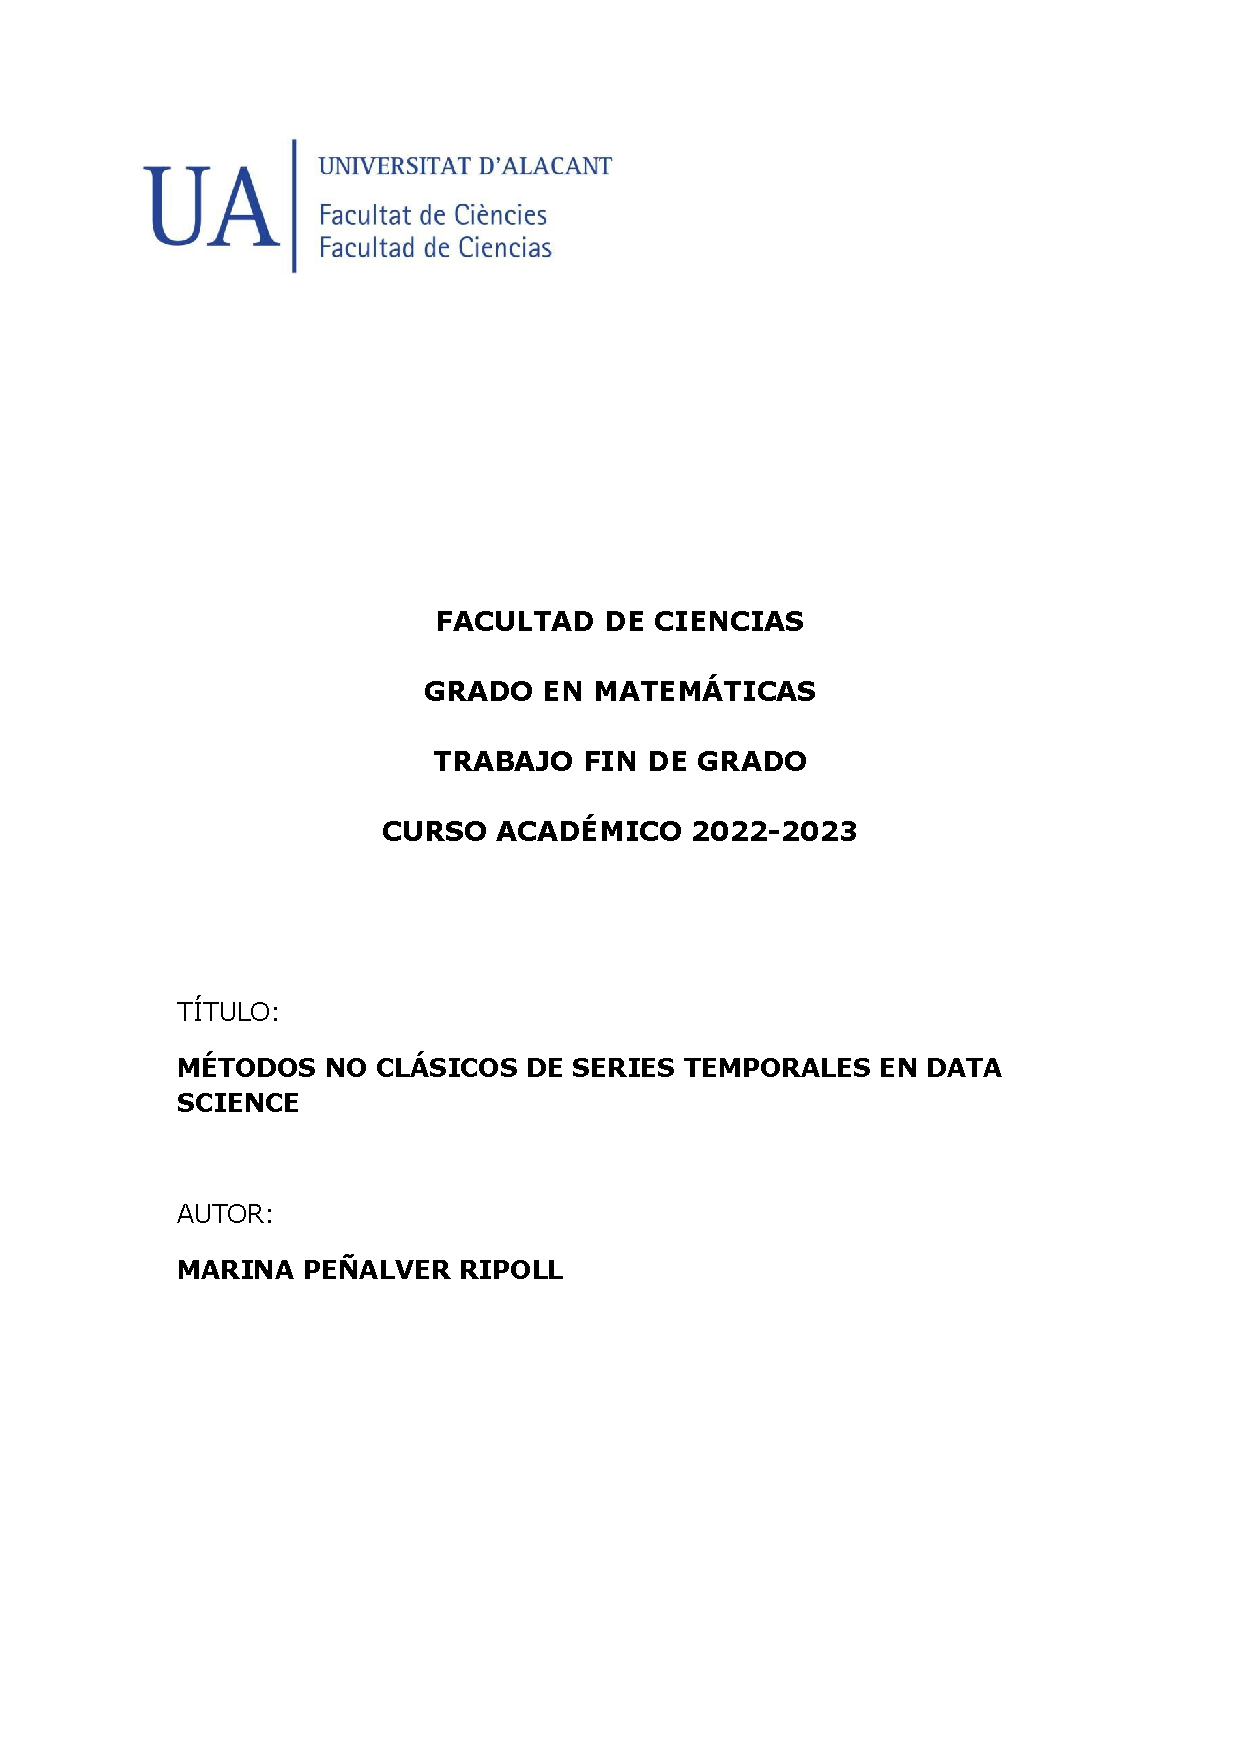
\includepdf[pages=1]{imagenes/anexo-1-portada-memoria-tfg-matematicas.pdf}

%-------------------------------------------------------------------------------------------------------





% RESUMEN
\section*{Resumen}
Una serie temporal es una sucesión de datos ordenados cronológicamente. El análisis de series temporales se centra en modelar su comportamiento y utilizar los modelos para producir predicciones.  El aumento en los datos disponibles ha provocado un incremento en la demanda de analistas de datos capaces de interpretar dicha información. 

En este trabajo, se ha estudiado las características más relevantes de las series temporales, profundizando en la descomposición de dichas series y diferentes métodos avanzados de predicción. 

Primeramente, se ha presentado las definiciones básicas de proceso estocástico y estacionariedad, así como la descomposición tradicional de las series, para introducir los métodos clásicos de series temporales. En particular, se ha desarrollado los procesos de media móvil integrados autorregresivos estacionales (SARIMA), que surgen a partir de los procesos de medias móviles (MA) y los procesos autorregresivos (AR). También se estudia los modelos de suavizado exponencial, centrándose el algoritmo de Holt-Winters. 

La segunda parte del trabajo se centra en algunos de los métodos de predicción surgidos recientemente. El algoritmo de Prophet, desarrollado por Facebook en 2017, es muy eficiente a la hora de trabajar con series temporales con fuertes relaciones de estacionalidad. Además, se analizan procesos autorregresivos utilizando métodos de Machine Learning.

Finalmente, se ha comparado los diferentes métodos empleados teniendo en cuenta la precisión de las predicciones, señalando las diferencias entre ellos. Todo el código usado se ha desarrollado en exclusiva para este trabajo y se encuentra disponible en el repositorio público de GitHub de la autora.

\textbf{Palabras clave:} Predicción, SARIMA, Suavizado exponencial, Método de Holt-Winters, Prophet, Machine Learning.

%-------------------------------------------------------------------------------------------------------


\newpage
% RESUMEN EN INGLÉS
\section*{Abstract}
Time series are a sequence of data ordered chronologically. Time series analysis focuses on modeling their behavior and using the models to produce predictions. The increase in available data has led to an increase in the demand for data analysts capable of interpreting such information. 

In this work, the most relevant characteristics of the time series have been studied, delving into the decomposition of time series and different prediction methods.

Firstly, the basic definitions of stochastic process and stationarity have been presented, as well as the traditional decomposition of the series, to introduce the classical methods of time series. In particular, seasonal autoregressive integrated moving average (SARIMA) processes have been developed, which arise from moving average (MA) and autoregressive (AR) processes. Exponential smoothing models are also studied, focusing on the Holt-Winters algorithm.

The second part of the work focuses on some of the forecasting methods that have recently emerged. Prophet's algorithm, developed by Facebook in 2017, is very efficient when it comes to working with time series with strong seasonal relationships. In addition, autoregressive processes are analyzed using Machine Learning methods.

Finally, the different methods used have been compared taking into account the precision of the predictions, pointing out the differences between them. All the code used has been developed exclusively for this work and is available in the author's GitHub repository.

\textbf{Key words:} Prediction, SARIMA, Exponential Smoothing, Holt-Winters, Prophet, Machine Learning.



%-------------------------------------------------------------------------------------------------------


\newpage
% ÍNDICE
\tableofcontents

%-------------------------------------------------------------------------------------------------------



\newpage
%INTRODUCCIÓN
\section{Introducción}
El mundo se actualiza a cada segundo, cada vez son más los dispositivos capaces de registrar y almacenar información.  Como consecuencia, los métodos y estrategias de análisis de datos han evolucionado para intentar entender y aprovechar dichos datos. El análisis de datos se ha convertido en una disciplina fundamental en el mundo actual, ya que gracias a él es posible entrenar modelos de aprendizaje para tomar decisiones, optimizar procesos o predecir resultados.

Una rama clave del análisis de datos es el análisis de series temporales, que son conjuntos de datos que se recopilan secuencialmente en intervalos de tiempo. Estos datos pueden ser observaciones de variables en diferentes momentos, como ventas diarias o registros de tráfico web. El análisis de series temporales se enfoca en descubrir patrones, tendencias y relaciones en estos datos a lo largo del tiempo.

A mediados del siglo XX empezaron a surgir diferentes métodos con el fin de modelar las series temporales. Dos de los procesos más populares en el día de hoy son los procesos autorregresivos (AR) y de medias móviles (MA), combinándolos se obtienen los procesos de media móvil autorregresivos (ARMA). El componente autorregresivo se refiere a la dependencia lineal que existe entre los valores pasados de una serie temporal y sus valores futuros, mientras que el componente de media móvil se utiliza para modelar los efectos de los errores. De esta forma se consigue modelar un tipo de procesos muy importante, los procesos estacionarios.

La evolución de los procesos no se quedó ahí, siguió evolucionando e incorporando nuevos componentes hasta que se propuso los modelos SARIMA (\emph{seasonal autoregressive integrated moving average}), además de las propiedades de los modelos ARMA también se le añade un componente estacional y los procesos integrados. Aunque estos no son los únicos procesos que surgieron, existen muchos otros como los VARIMA, ARARMA, este proyecto se centra en los SARIMA.

Otros de los métodos que tuvo una gran repercusión en el mundo de las series temporales es el suavizado exponencial, trabajo de Brown, Holt y Winters en los años 50 y 60. La técnica de suavizado exponencial se basa en la premisa de que los valores recientes de una serie temporal tienen más relevancia para la predicción que los valores más antiguos. De este modo, las predicciones se hacen asignando pesos exponenciales decrecientes a medida que se avanza el tiempo. Los métodos que se estudian en este trabajo son el método es alisado exponencial simple, el método lineal de Holt y el método del Holt-Winters, aunque existen muchos más.

Al igual que en todos los campos de la ciencia, el análisis de series temporales también ha evolucionado y nuevos modelos han sido creados. Muchos de estos nuevos métodos han surgido para compensar las limitaciones que presentan los métodos clásicos, que no son capaces de modelar los datos actuales, debido a su colosal dimensión o a otros factores. En este trabajo se estudia dos métodos surgidos recientemente.

En 2017, Facebook lanzó al público una algoritmo muy potente llamado Prophet \cite{Prophet1}, con el fin de afrontar una gran demanda de predicciones de calidad. Prophet tiene la ventaja de ser capaz de trabajar con datos de gran tamaño y modelar diferentes tipos de estacionalidad, lo cual es un punto débil en los métodos clásicos. Además, este algoritmo incorpora un componente muy interesante, los efectos de los días festivos, ya que hay ciertos días del año que pueden afectar a negocios y empresas. El objetivo de este trabajo es estudiar los componentes que se esconden detrás de este algoritmo e investigar cómo funciona, además de usarlo en un caso práctico.

El último método que se estudia son los modelos autorregresivos basados en árboles de decisión. A partir de los árboles de decisión es posible crear otros nuevos algoritmos de predicción mediante la agrupación de árboles. En este trabajo se estudia métodos como \emph{Random Forest} o \emph{XGBoost} modificados \cite{DT3} para poder predecir series temporales. 

Por último, se compara la actuación de todos los métodos aplicados a un mismo conjunto de datos, viendo las limitaciones y las ventajas de cada uno.





\subsection{La demanda eléctrica en Reino Unido}
Para desarrollar de manera práctica los algoritmos, se ha escogido un conjunto de datos llamado
``Electricity consumption UK 2009-2023''. Éste es un dataset formado por mediciones de la demanda eléctrica en Reino Unido desde enero de 2009 hasta abril de 2023. Se trata de un conjunto de datos público disponible en Kaggle (\href{https://www.kaggle.com/datasets/albertovidalrod/electricity-consumption-uk-20092022}{https://www.kaggle.com/ datasets/albertovidalrod/electricity-consumption-uk-20092022}). Los datos han sido tomados de forma diaria en intervalos de $30$ minutos, siendo $48$ observaciones al día, es decir en total hay $250800$ observaciones. La Tabla \ref{tab:dataset} muestra cómo están dispuestos los datos.
\begin{table}[h] 
\centering
\begin{tabular}{cc} \hline
    Date & Electricity Demand  \\ \hline
    01-01-2009 00:00 & 38704 \\
    01-01-2009 00:30 & 38965 \\
    $\vdots$ & $\vdots$ \\
    25-04-2023 23:00 & 26244 \\
    25-04-2023 23:30 & 25407 \\ \hline
\end{tabular}
\caption{Primeras y últimas observaciones del dataset
} \label{tab:dataset}
\end{table}

La predicción de la demanda eléctrica es esencial para la planificación y gestión eficiente de la generación y distribución de electricidad. Permite a las empresas eléctricas estimar la cantidad de energía que se requerirá en un período de tiempo dado, evitando así escasez o exceso de producción. Además, ayuda a los operadores de la red a equilibrar la oferta y la demanda en tiempo real, evitando sobrecargas o caídas en la red eléctrica y garantizando un suministro estable. 

A la hora de trabajar con los datos solo se ha tomado la variable que representa la demanda eléctrica, aunque el dataset es muy completo, para el análisis de series temporales es suficiente utilizar solo una variable, además de su identificador de fecha y hora.

El objetivo de este proyecto es encontrar modelos capaces de ajustar los datos, sin embargo la gran mayoría de los  métodos están limitados y el tiempo de ejecución es muy alto si se trabaja con los datos completos. Por esta razón, se ha resumido los datos, sumando los valores de las $48$ observaciones, obteniendo observaciones diarias. El reto de los modelos reside en capturar la tendencia a largo plazo, así como la estacionalidad anual, mensual y diaria.
\begin{figure}[h]
\centering
    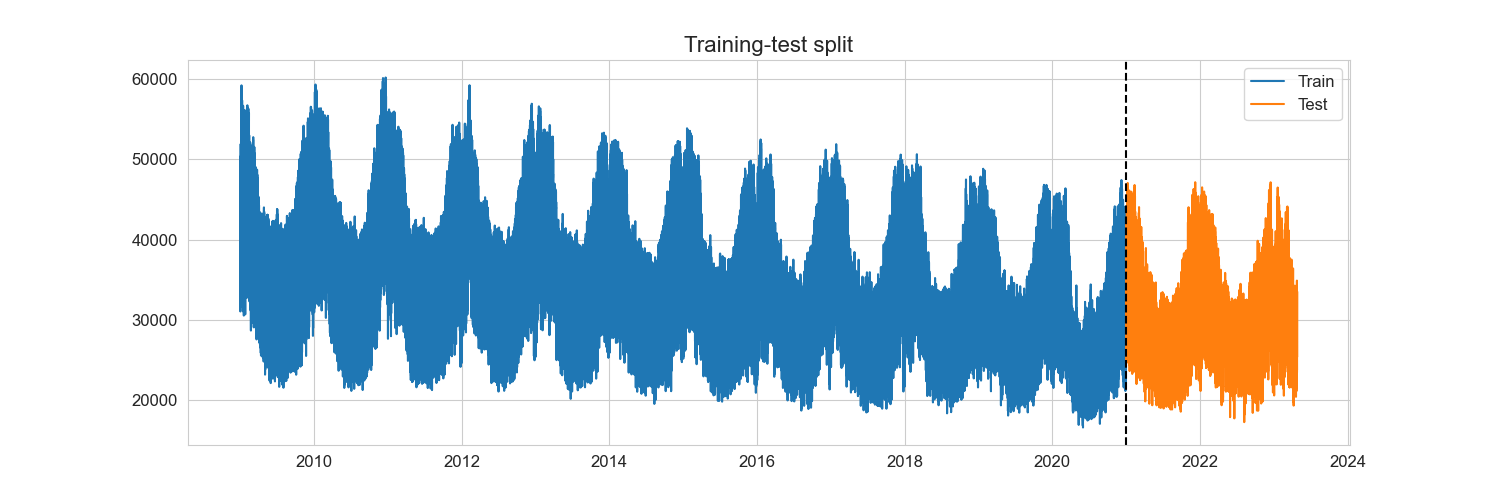
\includegraphics[width = \textwidth]{imagenes/train-test.png}
    \caption{Separación en conjuntos train y test para los datos agregados de manera diaria y completos, respectivamente}\label{train-test}
\end{figure}




Para aplicar los modelos se ha dividido el dataset en dos partes: conjunto de entrenamiento (train) y conjunto de testeo (test). El conjunto train consiste en los datos desde 2009 hasta 2020, inclusive.Y los datos del conjunto de test son todas las observaciones en adelante del 1 de enero de 2021. La Figura \ref{train-test} muestra la separación de los datos resumidos y los datos completos.


En la gráfica se ve que hay patrones que se repiten anualmente, pero también hay otros patrones, que se repiten mensualmente y semanalmente, y en el caso del dataset completo, diariamente. Se puede ver la estacionalidad diaria en la Figura \ref{fig:weekplot}.
\begin{figure}[h]
\centering
    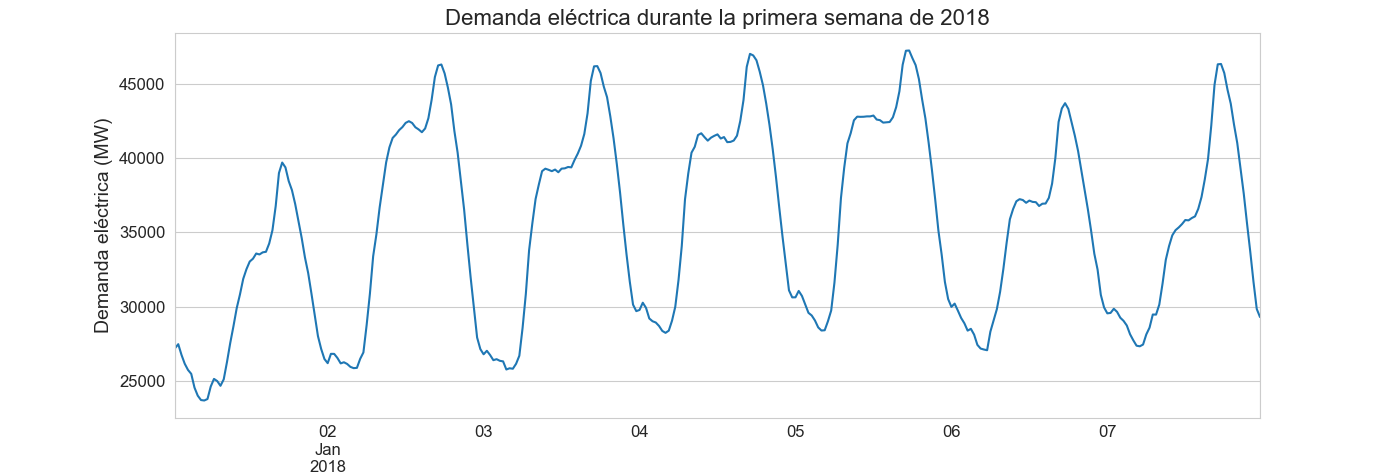
\includegraphics[width = 0.9\textwidth]{imagenes/weekplot.png}
    \caption{Estacionalidad diaria de los datos}\label{fig:weekplot}
\end{figure}

Asimismo, la estacionalidad no es el único factor a tener en cuenta a la hora de modelar series temporales. En el caso del algoritmo Prophet de Facebook, también tiene en cuenta los efectos de los días festivos y las vacaciones. Hay fechas señaladas que pueden afectar a los negocios o empresas que no son un día fijo del año, como el día de la madre o el \emph{Black Friday}. 
\begin{figure}[h]
\centering
    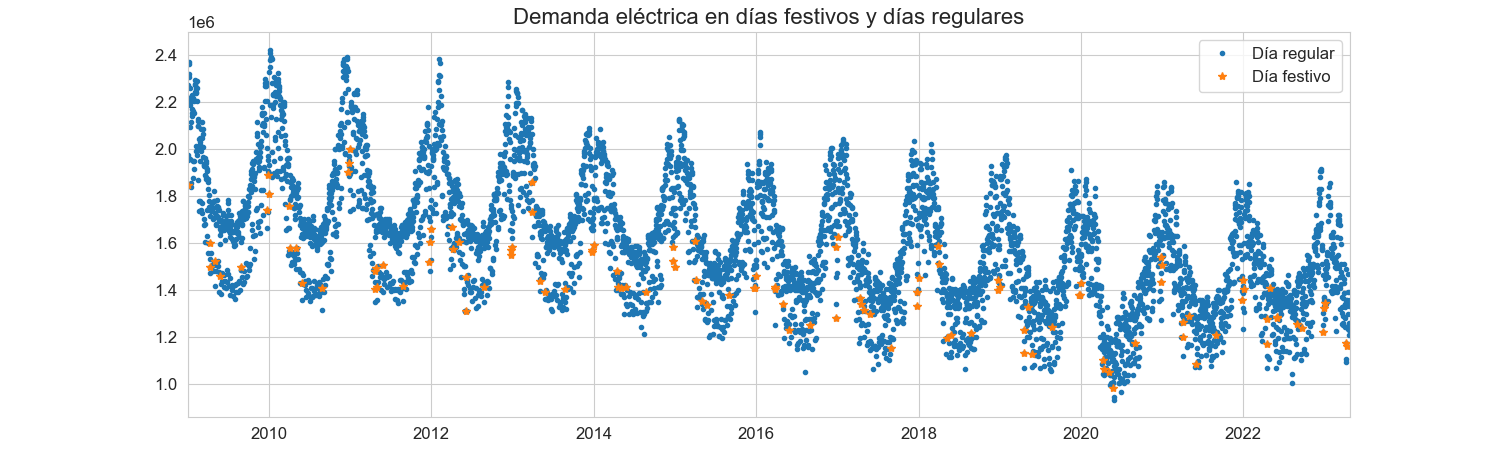
\includegraphics[width = \textwidth]{imagenes/hday.png}
    \caption{Días festivos en los datos diarios}\label{fig:hday}
\end{figure}

Esta clase de eventos pueden modificar los valores que toma una serie temporal. La Figura \ref{fig:hday} muestra los días festivos que contiene el dataset, mientras que la Figura \ref{fig:monthplot} es una comparación de la demanda eléctrica de los días festivos y los días regulares. Se puede observar que para los días festivos, en general, la demanda eléctrica disminuye.
\begin{figure}[h]
\centering
    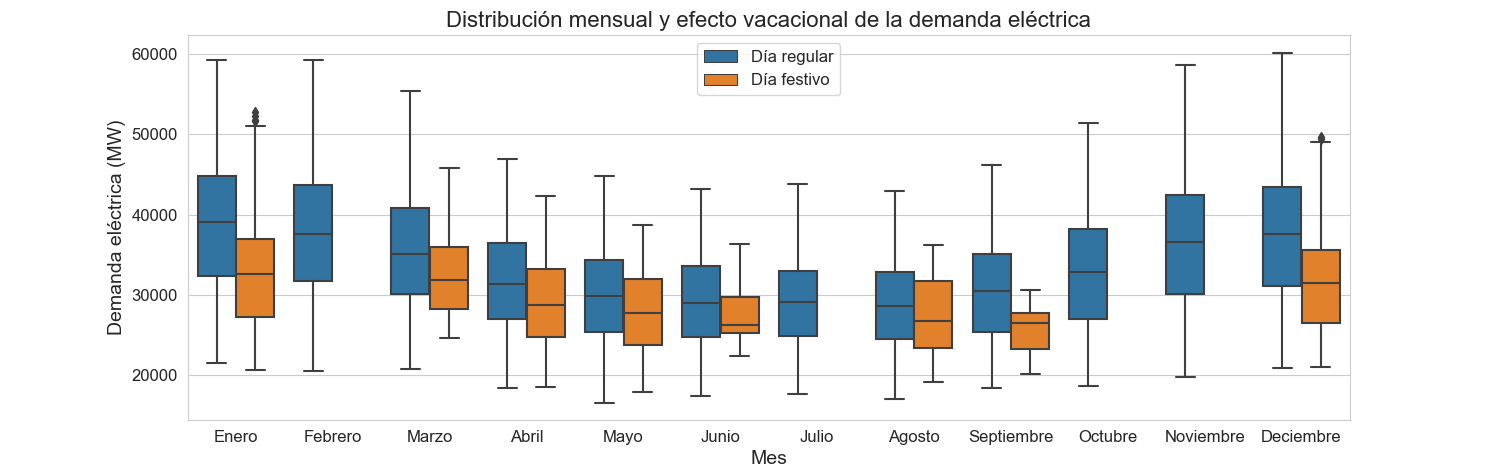
\includegraphics[width = 0.85\textwidth]{imagenes/monthplot.png}
    \caption{Comparación de la demanda eléctrica para días regulares y festivos}\label{fig:monthplot}
\end{figure}


\subsection{Evaluación y comparación de modelos}
A la hora de hacer predicciones se ha supuesto que se observa una serie temporal $\{X_1, \dotsc, X_T\}$ y se pretende predecir el valor de $X_{T+h}$. Con el fin de evaluar y comparar los modelos se ha utilizado el error absoluto medio porcentual (MAPE) y el error cuadrático medio (MSE). Las fórmulas de estos errores son
\begin{align*}
    \text{MAPE} \;=&\; \frac{1}{n}\sum_{i=1}^{n} \frac{\abs{\hat{X}_i - X_i}}{y_i}\cdot 100, \\
    \text{MSE} \;=&\; \frac{1}{n}\sum_{i=1}^n (\hat{X}_i - X_i)^2,
\end{align*}
donde $X_i$ son los valores reales e $\hat{X}_i$ son los valores pronosticados para los instantes de tiempo $i=1,\dotsc, n$, $n\in \mathbb{N}$. En este proyecto, los errores se calculan comparando datos del conjunto test contra los valores pronosticados por los modelos construidos con los datos de train. Al comparar los tiempos de ejecución de los modelos, el tiempo se ha medido en segundos.

Los modelos en los que el error del conjunto train es bajo y en el conjunto test es alto se dice que están sobreajustados (proviene del término en inglés \emph{overfitting}).




Todos estos efectos se estudian a lo largo del trabajo y en todo momento se pretende comprender cómo afectan estos componentes y encontrar los modelos óptimos capaces de ajustarse correctamente a los datos para predecir la demanda eléctrica. Todos los pasos y código empleado para realizar los modelos y gráficos del trabajo se encuentra en GitHub (\href{https://github.com/MarinaPenalver/TFG}{https://github.com/MarinaPenalver/TFG}).







\newpage
\section{Series temporales}
Una serie temporal es un conjunto de observaciones $x_t$, cada una registrada en un tiempo específico $t$. Una serie temporal con tiempo discreto es aquella en la que el conjunto de tiempo en los que se realizan las observaciones, $T_0$, es un conjunto discreto. Si los datos son medidos en intervalos fijados, por ejemplo mensual o anualmente, entonces es una serie temporal de tiempo discreto. En la Figura \ref{fig:TimeSeries} se muestra un gráfico de los datos, que es una serie temporal de tiempo discreto.

Este trabajo se centra en las series temporales de tiempo discreto, sin embargo también existen las de tiempo continuo. Las series temporales de tiempo continuo se obtienen cuando las observaciones son registradas de forma continua a lo largo del tiempo, por ejemplo, cuando $T_0 = [0,1]$. En este caso la notación pasa a ser $X(t)$, para así poder especificar que las observaciones son registradas de forma continua.


\begin{figure}[h]
\centering
    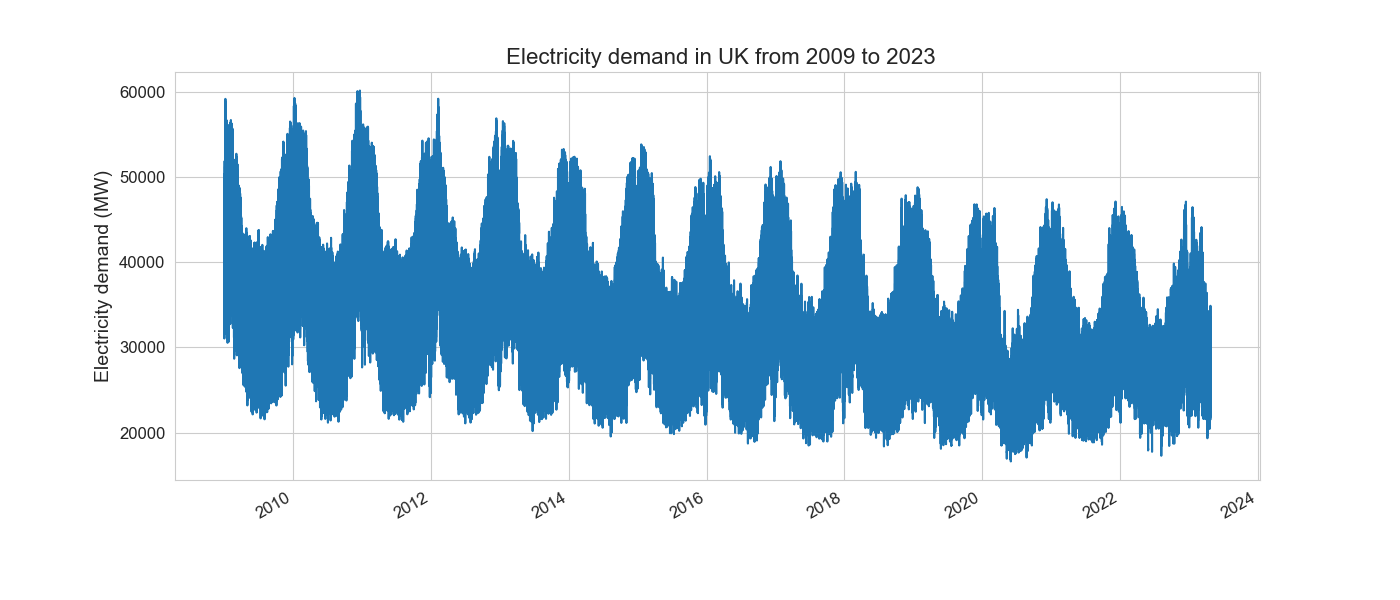
\includegraphics[width = \textwidth]{imagenes/TimeSeries.png}
    \caption{Serie temporal con tiempo discreto }\label{fig:TimeSeries}
\end{figure}





Se supone que cada observación $x_t$ es una realización de cierta variables aleatoria $X_t$. Una serie temporal $\{x_t, \, t \in T_0\}$ es una realización de una familia de variables aleatorias $\{X_t, \, t \in T_0\}$. Estas consideraciones sugieren modelar los datos como una realización (o parte de una realización) de un proceso estocástico $\{X_t, \, t \in T\}$ con $T_0 \subseteq T$.

\begin{definition}
    Un proceso estocástico es una familia de variables aleatorias $\{X_t, \, t \in T\}$ definidas en el espacio de probabilidad $(\Omega, \mathcal{F}, P)$, donde
    \begin{enumerate}
        \item $\Omega$ es el espacio muestral,
        \item $\mathcal{F} \subset \mathcal{P}(\Omega)$ es una $\sigma$-álgebra y 
        \item $P$ es la probabilidad, $P:\mathcal{F} \longrightarrow [0,1]$.
    \end{enumerate}
\end{definition}

En el análisis de series temporales el conjunto de índices $T$ es un conjunto de puntos, normalmente $\{0, \pm1, \pm2, \dotsc, \}$, $\{1,2,3,\dotsc\}$, $[0, \infty)$ o $(-\infty, \infty)$. Aunque también se puede definir procesos estocásticos en los cuales $T$ no es un subconjunto de $\mathbb{R}$.



\begin{remark}
    El término serie temporal se usa frecuentemente para referirse tanto a los datos como al proceso del cual es una realización.
\end{remark}


\subsection{Modelos estacionarios y estrictamente estacionarios}
A la hora de estudiar un número finito de variables, lo más común es usar la matriz de covarianzas para obtener información sobre la dependencia entre ellas. En el caso de las series temporales, es necesario extender este concepto para tratar con conjuntos infinitos de variables aleatorias. Esta extensión la proporciona la función de autocovarianzas.

\begin{definition}
    Si $\{X_t, \, t\in T\}$ es un proceso estocástico tal que $E(X_t^2)<\infty$ para todo $t\in T$, entonces la función de autocovarianzas $\gamma_X(\cdot, \cdot)$ de $\{X_t\}$ se define como
    \begin{equation}\label{eq:fun_autocov}
        \gamma(r,s) = Cov(X_r, X_s) = E[(X_r - E[X_r])(X_s-E[X_s])], \quad r,s \in T.
    \end{equation}
\end{definition}


\begin{definition}
     Si $\{X_t, \, t\in T\}$ es un proceso estocástico tal que $E(X_t^2)<\infty$, entontes
     \begin{enumerate}
         \item La función de autocorrelación simple (fas) se define como
         \begin{equation}\label{eq:ACF}
             \rho(r,s) = \frac{Cov(X_r, X_s)}{\sqrt{Var(X_r)(Var_s)}} = \frac{\gamma(r,s)}{\sqrt{\gamma(r,r) \gamma(s,s)}}.
         \end{equation}
         \item La función de autocorrelación parcial (fap) se define como
         \begin{equation}\label{eq:PACF}
             \alpha(r,s) = Corr(X_r, X_s \;\mid\; X_{r+1}, X_{r+2}, \dotsc, X_{s-1}) \quad \forall r < s.
         \end{equation}
     \end{enumerate}
\end{definition} 

\begin{figure}[h]
\centering
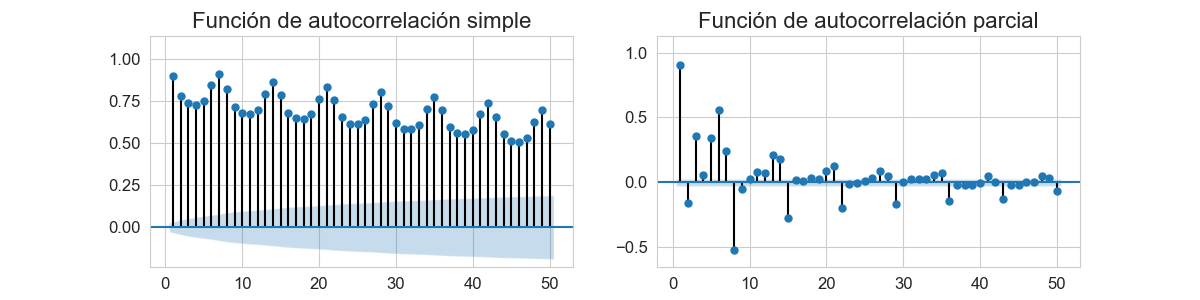
\includegraphics[width = 0.95\textwidth]{imagenes/ACF+PACF.png}
\caption{Funciones de autocorrelación de los datos diarios}\label{fig:ACF+PACF}
\end{figure}

% ?????
La Figura \ref{fig:ACF+PACF} muestra los gráficos de autocorrelación de los datos. Se puede ver que los coeficientes de correlación presentan máximos relativos para los múltiplos de siete, es decir, hay una fuerte relación en los días de la semana, y esta relación disminuye según las semanas están más separadas.
% ????




\begin{definition}\label{def:stationarity}
    Una serie temporal $\{X_t,\, t \in \mathbb{Z}\}$ se dice que es estacionaria si 
    \begin{enumerate}
        \item $E[X_t^2] <\infty$ $\forall t \in \mathbb{Z}$,
        \item $E[X_t] = \mu$ $\forall t \in \mathbb{Z}$,
        \item $\gamma(r,s) = \gamma(r+t, s+t)$ $\forall r,s,t \in \mathbb{Z}.$
    \end{enumerate}
\end{definition}

Esta definición de estacionariedad es referida habitualmente como estacionariedad débil. En este trabajo el término de estacionariedad se referirá siempre a la Definición \ref{def:stationarity}.


\begin{figure}[h]
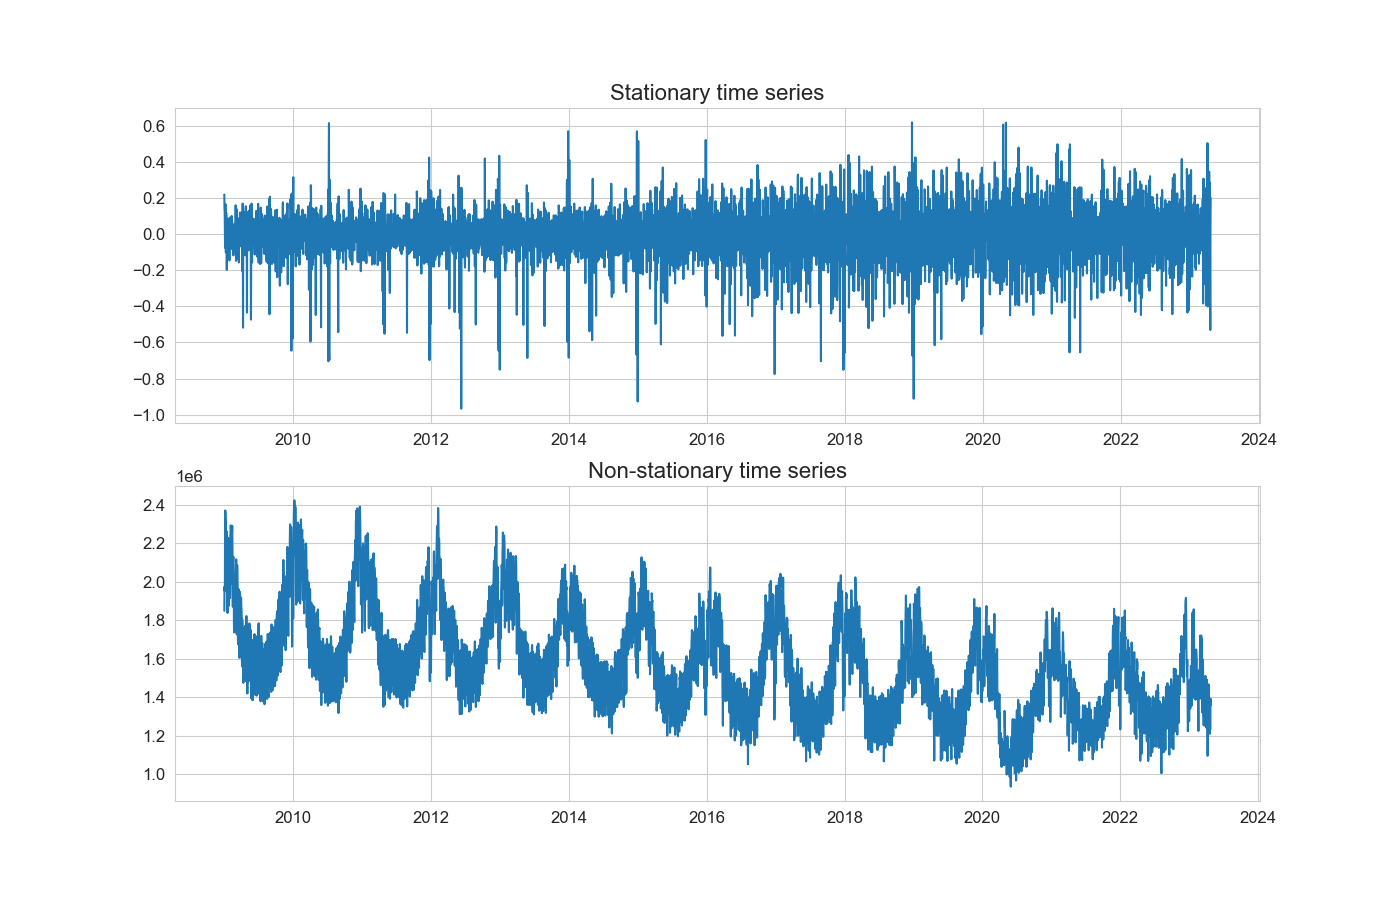
\includegraphics[width = \textwidth]{imagenes/Stationarity.png}
\caption{Ejemplos de serie estacionaria y no estacionaria, respectivamente.}\label{fig:Stationarity}
\end{figure}

La Figura \ref{fig:Stationarity} muestra dos ejemplos de series temporales: una estacionaria y otra no estacionaria. En el primer gráfico se observa que la media es cero y la varianza es constante, mientras que, en la segunda gráfica se ve que a lo largo de los años la media disminuye y hay patrones de repetición, es decir la media y la varianza no son constantes.


\begin{remark}
    Si $\{X_t, \,t \in \mathbb{Z}\}$ es estacionaria entonces $\gamma_X(r,s) = \gamma_X(r-s,0)$ para todo $r,s \in \mathbb{Z}$. Por tanto, es conveniente redifinir la función de autocovarianzas de un proceso estacionario como la función de una sola variable,
    \begin{equation*}
        \gamma_X(h) = \gamma_X(h,0) = Cov(X_{t+h}, X_t) \quad \text{para todo } t,h \in \mathbb{Z}.
    \end{equation*}
La función $\gamma_X(\cdot)$ hace referencia a la función de autocovarianzas de $\{X_t\}$ y $\gamma_X(h)$ a su valor para el retardo $h$. La función de autcorrelación simple de $\{X_t\}$ se define de forma análoga como función de un solo valor para el retardo $h$,
\begin{equation*}
    \rho_X(h) := \frac{\gamma_X(h)}{\gamma_X(0)} = Corr(X_{t+h}, X_t) \quad \forall t,h \in \mathbb{Z}.
\end{equation*}
\end{remark}


La definición de estacionariedad se ha dado para el caso en que $T = \mathbb{Z}$. No es difícil definir la estacionariedad usando un conjunto de índices más general, pero en este caso, no es necesario extender la definición. Si se quiere modelar un conjunto de datos $\{x_t, \, t\in T \subset \mathbb{Z}\}$ como una realización de un proceso estacionario, se puede considerar como parte de una realización de un proceso estacionario $\{X_t, \, t \in \mathbb{Z}\}$.


\begin{definition}[Estacionariedad estricta]\label{def:strictly_stationary}
    Una serie temporal $\{X_t, \,t \in \mathbb{Z}\}$ se dice estrictamente estacionaria si las distribuciones conjuntas $(X_{t_1}, \dotsc, X_{t_k})$ y $(X_{t_1+h}, \dotsc, X_{t_k+h})$ son la misma para todos los enteros positivos $k$ y para todo $t_1, \dotsc, t_k \in \mathbb{Z}$. 
\end{definition}

Si $\{X_t\}$ es estrictamente estacionaria, tomando $k=1$ en la Definición \ref{def:strictly_stationary} se tienen que $X_t$ tiene las misma distribución para todo $t \in \mathbb{Z}$. En particular, si $E[X_t^2] < \infty$, se tiene que $E[X_t]$ y $Var[X_t]$ son constantes. Además, para $k=2$ se tiene que $X_{t+h}$ y $X_t$ tienen la misma distribución conjunta para todo $h\in\mathbb{Z}$, y por consiguiente la misma covarianza. Por tanto, la estacionariedad estricta implica estacionariedad (débil).

% \begin{proposition}
%     Sea $\gamma(\cdot)$ la función de autocovarianza de un proceso estacionario $\{X_t, \; t \in T\}$, entonces se cumple:
%     \begin{enumerate}
%         \item $\gamma(0) \geq 0$.
%         \item $\abs{\gamma(h)} \leq \gamma(0)$, para todo $t\in T$.
%         \item $\gamma(h) = \gamma(-h)$, para todo $t\in T$.
%         \item $\gamma(\cdot)$ es definida no negativa, es decir, $\sum_{i,j=1}^n a_i \gamma(i-j) a_j \geq 0$ para $n\in \mathbb{N}$ y $(a_1, a_2, \dotsc, a_n)\in \mathbb{R}^n$.
%     \end{enumerate}
%     \begin{proof}
%         \begin{enumerate}
%             \item $\gamma(0) = Cov(X_t, X_t) = Var(X_t) \geq 0.$
%             \item Por la desigualdad de Cauchy-Schwarz...
%             \item $\gamma(-h) = Cov(X_{t-h}, X_t) = Cov(X_t, X_{t+h} = \gamma(h)$.
%             \item ...
            
%         \end{enumerate}
%     \end{proof}
% \end{proposition}





\subsection{Descomposición de una serie temporal}
En los métodos de descomposición clásica, los datos se generan como la suma de tres efectos,
\begin{equation}\label{eq:descom}
    X_t = \mu_t + S_t + Y_t,
\end{equation}
donde $\mu_t$ es el \emph{componente de tendencia}, $S_t$ es conocido como el \emph{componente estacional} y, por último, $Y_t$ es el componente puramente aleatorio o \emph{innovación}. En el caso de no presentar componente estacional, la descomposición se reduce a 
\begin{equation}\label{eq:descom2}
    X_t = \mu_t + Y_t.
\end{equation}

En la Figura \ref{fig:Decomposition} se muestra la decomposición aditiva  de los datos. Habitualmente, el nivel $\mu_t$ se modela mediante un polinomio del tiempo de orden menor o igual a dos, y la estacionalidad como una función periódica, que verifica la condición
\begin{equation*}
    S_t = S_{t-s},
\end{equation*}
donde $s$ es el periodo de la función. Una serie mensual con estacionalidad anual tiene periodo $s=12$ meses, ya que se supone que los \emph{coeficientes estacionales}, $S_t$, se repiten cada $12$ observaciones y una serie diaria con estacionalidad semanal tiene $s=7$ días.

La innovación es un componente aleatorio que recoge todos los demás efectos que actúan sobre la serie. Se supone que las variables aleatorias $Y_t$ tienen una estructura estable a lo largo del tiempo: media cero, varianza constante y distribución normal. Además, las observaciones correspondientes a dos periodos distintos de tiempo son independientes, es decir, conocer el valor $Y_t$ no proporciona ninguna información sobre el posible valor de $Y_{t+1}$.



\begin{figure} 
    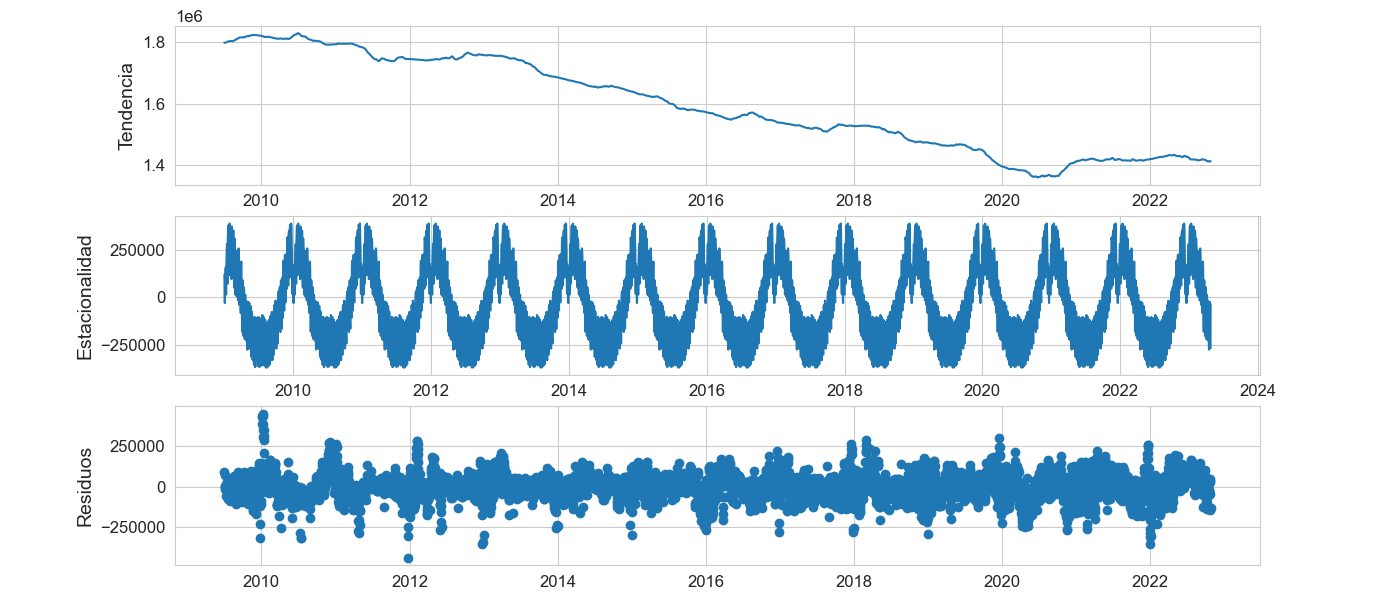
\includegraphics[width = \textwidth]{imagenes/Decomposition.png}
    \caption{Descomposición aditiva de los datos}\label{fig:Decomposition}
\end{figure}



Una alternativa a la descomposición aditiva es la descomposición multiplicativa, que consta de los mismos componentes, y también es muy utilizada, 
\begin{equation}\label{eq:descom3}
    X_t = \mu_t \times S_t \times Y_t.
\end{equation}

En este caso la componente de tendencia y la de estacionalidad se combinan multiplicativamente junto con el componente aleatorio.

% \begin{figure}
%     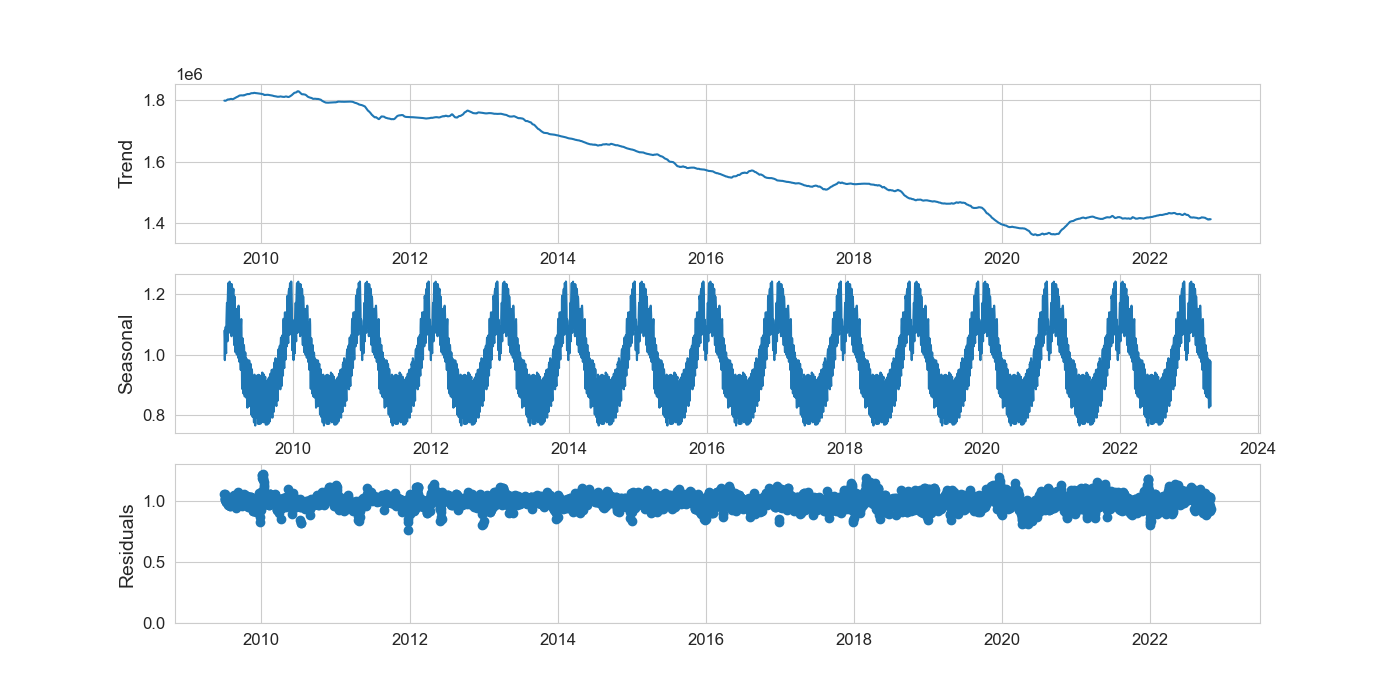
\includegraphics[width = \textwidth]{imagenes/Decomposition2.png}
%     \caption{Descomposición multiplicativa de los datos}\label{fig:Decomposition2}
% \end{figure}


\newpage
\section{Procesos autorregresivos y de media móvil}
En esta sección se estudia una clase muy importante de series temporales, definida en términos de ecuaciones en diferencias lineales con coeficientes constantes. La imposición de esta estructura adicional define una familia de procesos estacionarios, los llamados procesos de media móvil autorregresivos o ARMA. Antes de estudiar dichos procesos, es necesario introducir un nuevo tipo de proceso, el proceso de ruido blanco.


\begin{definition}\label{def:WN_process}
    El proceso $\{Y_t\}$ se conoce como proceso de ruido blanco con media $0$ y varianza $\sigma^2$,
    \begin{equation} \label{eq:WN_process}
        \{Y_t\} \sim \text{WN}(0, \sigma^2),
    \end{equation}
    si $\{Y_t\}$ tiene media $0$ y función de autocovarianza
    \begin{equation} \label{eq:WN_autocov}
        \gamma(h) = 
        \left\{ \begin{array}{ll} 
        \sigma^2 & \text{si } h=0 \\
        0 & \text{si } h \neq 0 
        \end{array} \right.
    \end{equation}

    Si las variables aleatorias $Y_t$ son independientes e idénticamente distribuidas con media $0$ y varianza $\sigma^2$, entonces se conocen como
    \begin{equation} \label{eq:IDD_process}
        \{Y_t\} \sim \text{IID}(0, \sigma^2).
    \end{equation}
\end{definition}

Los procesos de ruido blanco permiten generar una clase muy amplia de procesos estacionarios gracias a ecuaciones en diferencias lineales.

\begin{definition}\label{def:ARMA}
    El proceso $\{X_t, \,t\in T\}$ se dice $\arma(p,q)$ si es estacionario y para todo $t$, 
    \begin{equation}\label{eq:ARMA}
        X_t - \phi_1X_{t-1}-\dotsb-\phi_pX_{t-p} = Y_t +\theta_1Y_{t-1} + \dotsb + \theta_q Y_{t-q},
    \end{equation}
    donde $\{Y_t\}\sim \wn$. Se dice que $\{X_t\}$ es un proceso $\arma(p,q)$ con media $\mu$ si $\{X_t - \mu\}$ es un proceso $\arma(p,q)$.
\end{definition}

La ecuación \eqref{eq:ARMA} puede escribirse de forma más compacta, introduciendo la notación del operador de retardo.

\begin{definition}\label{def:lag_operator}
    Se llama operador de retardo a $B$, definido por  
    \begin{equation}\label{eq:lag_operator}
    BX_t = X_{t-1}.
\end{equation}
Además cumple las propiedades siguientes:
\begin{enumerate}
    \item $B\mu = \mu$, para $\mu$ constante.
    \item $B a X_t = a B x_t = aX_{t-1}$, para $a$ constante.
    \item Es lineal, es decir, $B(af(t) + bg(t)) = af(t-1) + b g(t-1)$.
    \item $B^kX_t = \underbrace{B\cdots B}_k X_t = X_{t-k}$.
\end{enumerate}
\end{definition}

Utilizando la notación del operador de retardo, la ecuación \eqref{eq:ARMA} puede escribirse como
\begin{equation}\label{eq:ARMA_lag_op}
    \phi(B)X_t = \theta(B)Y_t,
\end{equation}
donde $\phi(B)$ y $\theta(B)$ son polinomios de grado $p$ y $q$ en el operador de retardo,
\begin{align}
    \phi(B) =& \;1 - \phi_1 B - \dotsb - \phi_p B^p \label{eq:ar_lag_op}, \\
    \theta(B) =&\; 1 +\theta_1 B + \dotsb + \theta_q B^q \label{eq:ma_lag_op}.
\end{align}

A $\phi(B)$ se le conoce como el operador del proceso autorregresivo u operador AR y a $\theta(B)$ se le conoce como el operador del proceso de media móvil u operador MA. El proceso $\arma(p,q)$ es estacionario si, y sólo si, el módulo de las raíces de $\phi_p(B) = 0$ son mayores a $1$.

\begin{remark}
Para cualquier función de autocovarianza $\gamma(\cdot)$ tal que $\lim_{h\rightarrow\infty} \gamma(h) = 0$, y para todo entero $k>0$, es posible encontrar un proceso ARMA con función de autocovarianza $\gamma_X(h) = \gamma(h)$ con $h=0,1\dotsc,k$. 
\end{remark}
Por razones como esta, la familia de los procesos ARMA juega un papel muy importante en la modelación de series temporales. Además, su estructura lineal conduce a una teoría simple de predicciones lineales.


\begin{example}[Proceso $\ma(q)$]
    Si $\phi(B) \equiv 1$, entonces
    \begin{equation}\label{eq:ma_process}
        X_t = \theta(B)Y_t,
    \end{equation}
    y a este proceso se le conoce como proceso de media móvil de orden $q$ o $\ma(q)$ por sus siglas en inglés, \emph{moving average}. Se tiene que $\{X_t\}$ es estacionaria ya que, tomando $\theta_0 = 1$ y $\theta_j = 0$ para $j > q$, se tiene que, $\forall h > 0$
    \begin{align*}
        E[X_t] & = \sum_{j=0}^q \theta_j E[Y_{t-j}] = 0 \quad \text{y}\\
        \gamma_X(h) = Cov(X_{t+h}, X_t) & = \left\{\begin{array}{ll}
            \sigma^2 \sum_{j=h}^{q} \theta_j \theta_{j - h} & \text{si } h \leq q,  \\
            0 & \text{si } h > q.
        \end{array}\right.
    \end{align*}
\end{example}

\begin{example}[Proceso $\ar(p)$] Si $\theta(B)\equiv1$, entonces
\begin{equation}\label{eq:ar_process}
    \phi(B)X_t = Y_t
\end{equation}
y a este proceso se le conoce como proceso autorregresivo de orden $p$ o $\ar(p)$. Este proceso es estacionario solo si las raíces de $\phi(B) = 0$ están fuera del círculo unidad.
\end{example}


\subsection{Procesos ARIMA}
Se puede definir nuevos procesos no estacionarios a partir de la Definición \ref{def:ARMA}. Para ello, se incorporan raíces unitarias al proceso ARMA a través de un operador.


\begin{definition}
    El operador de diferenciación, denotado por $\nabla$, se define como
    \begin{equation*}
        \nabla = 1 -B.
    \end{equation*}
\end{definition}

De igual modo, se define el operador de diferenciación de orden $s$ u operador de diferenciación estacional como $\nabla_s = 1 - B^s$. Con los operadores se puede definir un nuevo proceso.

\begin{definition}
    Se dice que $\{X_t\}$ es un proceso integrado de orden $h$, $I(h)$, si al diferenciar $\{X_t\}$ $h$ veces se obtiene un proceso estacionario.
\end{definition}

Uniendo los procesos estudiados, es decir los $\arma(p,q)$ con los procesos integrados, se obtiene los procesos de media móvil integrados autorregresivos o ARIMA.

\begin{definition}
    Se dice que $\{X_t\}$ es un proceso $\arima(p,d,q)$ si
    \begin{equation}\label{eq:ARIMA}
        \phi(B)(1-B)^d X_t = \theta(B) Y_t
    \end{equation}
    o, con la notación del operador de diferenciación
        \begin{equation}\label{eq:ARIMA2}
        \phi(B)\nabla^d X_t = \theta(B) Y_t,
    \end{equation}
    donde $\{Y_t\} \sim \wn$, $\theta(B) = 1 + \theta_1B + \dotsb + \theta_qB^q$, $\phi(B) = 1 - \phi_1B - \dotsb - \phi_qB^p$ y las raíces de $\phi(B) = 0$ tienen módulo mayor que 1.
\end{definition}

Por la estructura de los procesos ARIMA, se sabe que son no estacionarios, sin embargo se puede definir $W_t = \nabla^d X_t$ que es un proceso $\arma(p,q)$ y sí es estacionario.

\subsection{Procesos SARIMA}\label{sec:SARIMA}
Los procesos ARIMA pueden enriquecerse añadiendo un componente multiplicativo autorregresivo para capturar la estacionalidad, dando como resultado el modelo SARIMA.
\begin{definition}
    $\{X_t\}$ es un proceso ARIMA multiplicativo estacional o SARIMA, denotado $\{X_t\} \sim \arima(P,D,Q)_s\times (p,d,q)$, si
    \begin{equation}\label{eq:SARIMA}
        \Phi(B^s)\phi(B) \nabla_s^D \nabla^d X_t = \theta(B) \Theta(B^s) Y_t,
    \end{equation}
    donde
    \begin{itemize}
        \item $\{Y_t\} \sim \wn$,
        \item $\nabla_s^D$ representa la diferenciación estacional,
        \item $\nabla^d$ representa la diferenciación regular,
        \item $\Phi(B^s) = 1 - \Phi_1B^s - \dotsb - \Phi_PB^{sP}$ es el operador AR estacional,
        \item $\phi(B) = 1 - \phi_1B - \dotsb - \phi_pB^p$ es el operador AR,
        \item $\Theta(B^s) = 1 + \Theta_1B^s + \dotsb + \Theta_QB^{sQ}$ es el operador MA estacional,
        \item $\theta(B) = 1 + \theta_1B + \dotsb + \theta_qB^q$ es el operador MA.
    \end{itemize}
\end{definition}


% \subsubsection{Predicciones del modelo SARIMA}
En la siguiente parte de esta sección se explica cómo calcular las predicciones del modelo SARIMA y se estudia los resultados obtenidos a partir de los datos.

Al predictor de $X_{T+h}$ con origen $T$ y horizonte de la predicción $h$ se le conoce como $\hat{X}_T(h)$, es decir, $\hat{X}_T(h)$ se calcula en función de los $T$ valores observados de la serie. Si la predicción es lineal entonces se puede escribir como
\begin{equation*}
    \hat{X}_T(h) = \alpha_1X_T + \alpha_2X_2 + \dotsb + \alpha_T X_1.
\end{equation*}
El predictor queda definido al determinar el valor de las constantes $\alpha_1, \alpha_2, \dotsc ,\alpha_T$. El predictor lineal que minimiza el error cuadrático medio, $$\text{MSE}(\hat{X}_T(h)) = E[(\hat{X}_T(h) - X_{T+h})^2 \mid  X_1, \dotsc, X_T\,],$$ es 
\begin{equation} \label{eq:best_predictor}
    \hat{X}_T(h) = E[X_{T+h}\mid X_1, \dotsc, X_T\,].
\end{equation}

Supóngase que $\{X_t\} \sim \arima(P,D,Q)_s \times (p,d,q)$, se ha observado $x_1, x_2, \dotsc, x_T$ y se pretende calcular la predicción de $X_{T+h}$, con $h\in \mathbb{N}$. Para $D=1$, es posible calcular las predicciones de forma sencilla pues se tiene que el predictor lineal de \eqref{eq:best_predictor} cumple la ecuación
\begin{equation}\label{eq:SARIMA_pred1}
    \Phi_P(B^s) \phi_p(B) \nabla_s \nabla^d \hat{X}_T(h) = 0,\quad h > q+ sQ.
\end{equation}

Defininiendo el operador estacional puro, $S_s(B) = 1 + B + \dotsb + B ^{s-1}$, la ecuación \eqref{eq:SARIMA_pred1} se puede escribir como
\begin{equation}\label{eq:SARIMA_pred2}
    \Phi_P(B^s) \phi_p(B) S_s(B) \nabla^{d+1} \hat{X}_T(h) = 0,\quad h > q+ sQ.
\end{equation}

En consecuencia, para $h\geq \max(1, q + sQ + 1 - (d+s+p+sP))$ las predicciones $\hat{X}_T(h)$ son las soluciones de la ecuación en diferencias \eqref{eq:SARIMA_pred2} y se tiene que
\begin{equation}\label{eq:SARIMA_pred3}
    \hat{X}_T(h) = T_T(h) + S_T(h) + t_T(h),
\end{equation}
donde
\begin{enumerate}
    \item $T_T(h)$ es el componente de tendencia, solución de $(1-B)^{d+1}T_T(h)=0$. $T_T(h)$ es un polinomio de grado $d$ con coeficientes que se adaptan a lo largo del tiempo.
    \item $S_T(h)$ es el componente estacional, solución de $S_s(B)S_T(h)$. $S_T(h)$ es una función de periodo $s$ tal que $\sum_{j=1}^s S_T(j)=0$.
    \item $t_T(h)$ es el componente transitorio, solución de $\Phi(B^s)\phi(B)t_T(h)=0$. $t_T(h)$ está determinado por las raíces de los operadores regular y estacional autorregresivos.
\end{enumerate}





La implementación en Python de este método se ha hecho gracias al paquete \texttt{statsmodels}, aplicado a los datos diarios, ya que si se tomara el dataset completo el tiempo de ejecución ascendería hasta horas o días. La Figura \ref{fig:SARIMA} muestra tanto los datos ajustados como las predicciones. 

\begin{center}
\begin{figure}[h]
    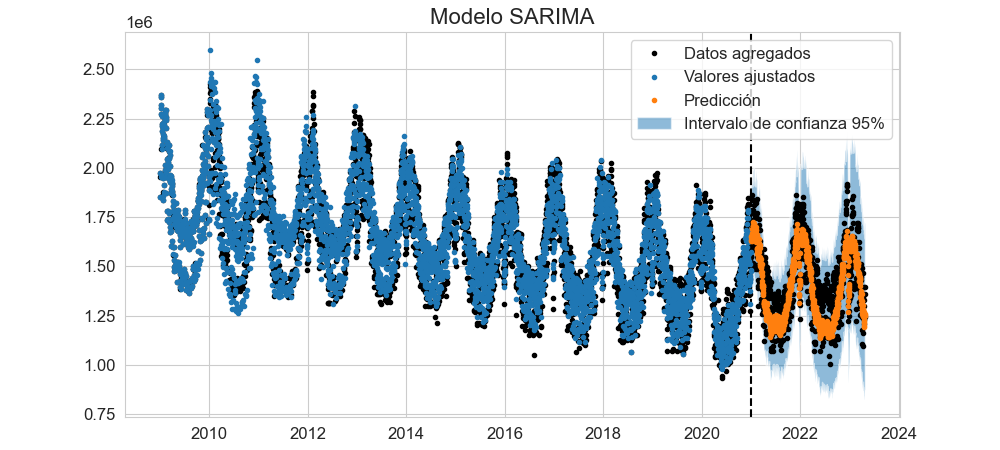
\includegraphics[width = 0.95\textwidth]{imagenes/SARIMA.png}
    \caption{Modelo ajustado con SARIMA}\label{fig:SARIMA}
\end{figure}
\end{center}

En el conjunto de entrenamiento, los datos se ajustan correctamente, especialmente en el primer año de la serie, pero según se avanza en el tiempo, el modelo, a través de su componente estacional aditivo, no alcanza los extremos estacionales de la serie.

Exactamente lo mismo ocurre en los datos de testeo, pero en la Figura \ref{fig:SARIMA_pred} se ve cómo la predicción permanece aproximadamente en la media de todas las observaciones. El intervalo de confianza del $95\%$ sí logra capturar todas las observaciones en su interior. Además, conforme se avanza en el tiempo, el intervalo de confianza también aumenta su amplitud, siendo cada vez menos preciso, como es lógico. 

\begin{figure}[h]
\centering
    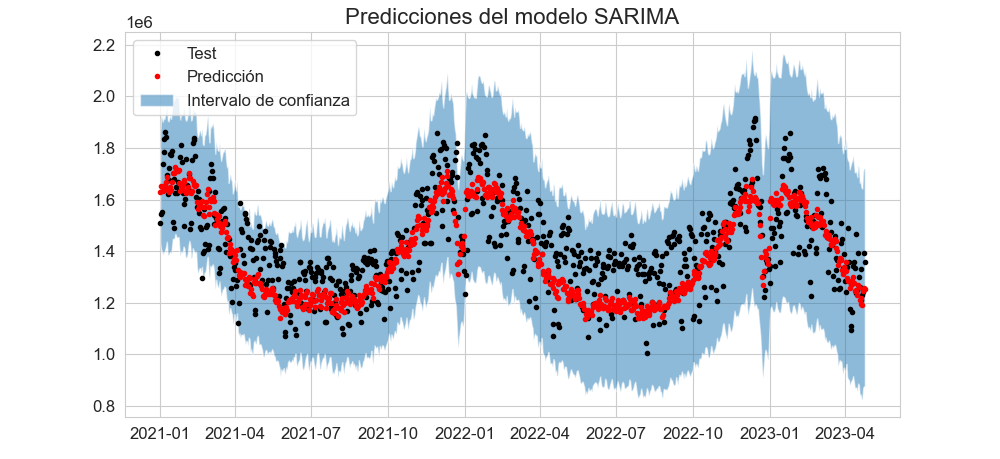
\includegraphics[width = 0.95\textwidth]{imagenes/SARIMA_pred.png}
    \caption{Predicciones con SARIMA}\label{fig:SARIMA_pred}
\end{figure}



De este modelo, cabe destacar que el error absoluto medio porcentual es del $14.31\%$, el error MSE y su tiempo de ejecución se puede observar en la Tabla \ref{tab:SARIMA}. El error porcentual no es significativamente grande, pero el modelo no es capaz de capturar los patrones estacionales que no son anuales, pues en este caso también hay estacionalidad semanal y mensual, y con los modelos SARIMA solo es posible ajustar a un tipo de estacionalidad.

\begin{table}[h]
    \centering
    \begin{tabular}{ccc} \hline
         MAPE & MSE & Tiempo \\ \hline
         $14.31\%$ &  $1.761 \cdot 10^{10}$ & $1104$ \\ \hline
    \end{tabular}
    \caption{Errores y tiempo de ejecución del modelo SARIMA}
    \label{tab:SARIMA}
\end{table}


Se ha utilizado la metodología de Box-Jenkins \cite{TS4} para identificar el modelo SARIMA que se ajusta a los datos. El modelo presentado en la imagen es un proceso $\arima(1,1,2)_{365}\times(1,1,1)$, los valores de los parámetros se encuentran en la Tabla \ref{tab:SARIMA2}. La limitación de este método es su tiempo de ejecución. Al ser el periodo de estacionalidad $s=365$, la duración de computación del algoritmo es grande, además si se aumenta el número de parámetros de los procesos AR y MA, el tiempo de computación es tan alto que es inviable calcularlo.

\begin{table}[h] 
\centering
\begin{tabular}{cccccc} \hline
    $\phi_1$ & $\theta_1$ & $\theta_2$ & $\Phi_1$ & $\Theta_1$ & $\sigma^2$  \\ \hline
    $0.0634$ & $-0.2977$  & $-0.6445$  & $0.1278$ & $-0.9998$  & $393.9037$ \\ \hline
\end{tabular}
\caption{Parámetros de modelo SARIMA} \label{tab:SARIMA2}
\end{table}


El fundamento de la metodología de Box-Jenkins se basa en proponer diferentes modelos gracias a los gráficos de las funciones de autocorrelación para después escoger el que mejor se ajuste. En este caso, no se ha podido computar todos los modelos, por exceso de tiempo computacional. Si se trabaja con estacionalidad $s=7$ o $s=30$ para datos semanales o mensuales, respectivamente, el algoritmo obtiene la solución en segundos o minutos. No obstante, el objetivo es trabajar con los datos disponibles y estacionalidad que le corresponde, de forma que este modelo no es adecuado en este caso.

En consecuencia, el modelo SARIMA funciona correctamente, pero existen otros modelos con menor coste computacional que podrían ajustar los datos de forma más precisa, teniendo en cuenta diferentes tipos de estacionalidad de forma simultánea. En las siguientes secciones se presenta algunos de esos métodos.

La implementación en Python se ha realizado con la función \texttt{ARIMA} del paquete \texttt{statsmodels}, aunque también existe otra función que encuentran un modelo que minimiza un error dado. Esta función se conoce como \texttt{auto.arima} y permite evitar los pasos de la metodología de Box-Jenkins, pues el propio algoritmo propone diferentes modelos y calcula su error. En este caso, no se ha usado esta función, debido al tiempo de ejecución, pero en ciertos casos puede ser útil para ahorrar el tiempo de identificación de modelos al analista de datos o incluso para proponer modelos que el analista no ha contemplado.

La función \texttt{ARIMA} permite crear modelos a partir de los parámetros referentes los órdenes de los operador, \texttt{order(p,d,q)} y \texttt{seasonal\_order(P,D,Q,s)} y, además, es posible añadir variables exógenas a la serie con el parámetro \texttt{exog}.

La inclusión de variables exógenas permite capturar relaciones y efectos que no están directamente relacionados con la serie temporal en sí, pero que pueden tener un impacto en su comportamiento. 

Entrenar un modelo con una variable exógena provoca que esa variable sea necesaria también para generar las predicciones, pero no se conoce el valor de la variable exógena en un futuro. Una forma de solventar este problema es utilizar el algoritmo correspondiente para predecir la variable exógena, en este caso el modelo SARIMA. De este modo, se puede predecir la variable deseada a partir de las predicciones de la variable exógena y del modelo entrenado con los datos y la variable exógena.







\newpage
\section{Suavizado exponencial}

El suavizado o alisado exponencial describe una clase de métodos de predicción. De hecho, muchos de los métodos de predicción más exitosos están basados en el concepto del suavizado exponencial. Hay una gran variedad de métodos basados en esta familia, cada una con la propiedad de que los pronósticos son combinaciones ponderadas de observaciones pasadas, donde las observaciones recientes tienen  más peso que las observaciones más alejadas. El nombre ``suavizado exponencial'' refleja el hecho de que los pesos caen exponencialmente según las observaciones son más lejanas.

En este capítulo se va a estudiar tres de los métodos más reconocidos en la familia de suavizado exponencial: el método de suavizado simple, el método lineal de Holt y el método de Holt-Winters. Todos estos algoritmos están implementados en Python en el paquete \texttt{statsmodels} \cite{ES4}.




\subsection{Suavizado exponencial simple}
El modelo de suavizado exponencial simple recibe su nombre por ser el más sencillo de esta familia. Esta técnica solo se puede aplicar a datos que no presentan tendencia ni patrones estacionales. 

El método de \textit{simple exponential smoothing}, resultado del trabajo de Robert Goodell Brown \cite{ES1} en la década de los 50, toma la predicción del periodo previo y lo ajusta usando el error de predicción.

Si se supone que se dispone de las observaciones hasta $T-1$ y se quiere predecir el próximo valor de la serie temporal $X_T$, entonces el error de la predicción es $X_T - \hat{X}_T$, siendo $\hat{X}_T$ la predicción. En el método de suavizado exponencial simple la predicción para el siguiente tiempo se define como
\begin{equation} \label{eq:simple_exp}
   \hat{X}_{T+1} = \hat{X}_T + \alpha (X_T - \hat{X}_T), 
\end{equation}

donde $\alpha$ es una constante entre $0$ y $1$.

La nueva predicción es la predicción anterior sumando un ajuste para el error de la última predicción. Cuando $\alpha$ tiene un valor cercano a $1$, la nueva predicción tendrá un ajuste significativo por el error en la anterior predicción. Por el contrario, cuando $\alpha$ es cercano a $0$, el nuevo pronóstico tendrá un ajuste muy pequeño.

Otra forma de escribir la ecuación \eqref{eq:simple_exp} es
\begin{equation} \label{eq:simple_exp2}
    \hat{X}_{T+1} = \alpha X_T + (1-\alpha)\hat{X}_T. 
\end{equation}

La predicción $\hat{X}_{T+1}$ está basada en la ponderación de la observación más reciente, $X_T$ con un peso de $\alpha$ y la predicción más reciente, $\hat{X}_T$ con peso de $1-\alpha$. Las implicaciones del suavizado exponencial se pueden observar más fácilmente si se expande la ecuación \eqref{eq:simple_exp2} sustituyendo $\hat{X}_T$ por sus componentes, como sigue:
\begin{equation*}
\begin{split}
\hat{X}_{T+1} & =  \alpha X_T + (1-\alpha) [\alpha X_{T-1} + (1-\alpha)\hat{X}_{T-1}] \\
& = \alpha X_T + \alpha(1-\alpha)X_{T-1} + (1-\alpha)^2\hat{X}_{T-1}.
\end{split}
\end{equation*}

Si se repite este proceso de sustitución de $\hat{X}_{T-1}$ por sus componentes, $\hat{X}_{T-2}$ por sus componentes, y así, se llega al resultado
\begin{equation*}
\begin{split}
    \hat{X}_{T+1} = &\; \alpha X_T + \alpha(1-\alpha)X_{T-1} + \alpha(1-\alpha)^2X_{T-2} + \alpha(1-\alpha)^3X_{T-3} \\
    & + \alpha(1-\alpha)^4X_{T-4} + \dotsb +  \alpha(1-\alpha)^{T-1}X_1 + (1-\alpha)^T\hat{X}_1.
\end{split}
\end{equation*}

Por tanto $\hat{X}_{T+1}$ representa un promedio móvil ponderado con todas las observaciones pasadas y los pesos decreciendo exponencialmente, de ahí el nombre de ``suavizado exponencial''.

El pronóstico para cualquier horizonte $h$ se calcula como
\begin{equation}
    \hat{X}_{T+h} = \hat{X}_{T+1},
\end{equation}
es decir, las predicciones a largo plazo son planas, por esta razón el método de suavizado exponencial simple se utiliza con datos que no presentan tendencia, estacionalidad ni otros patrones.


\begin{figure}[h]
    \centering
    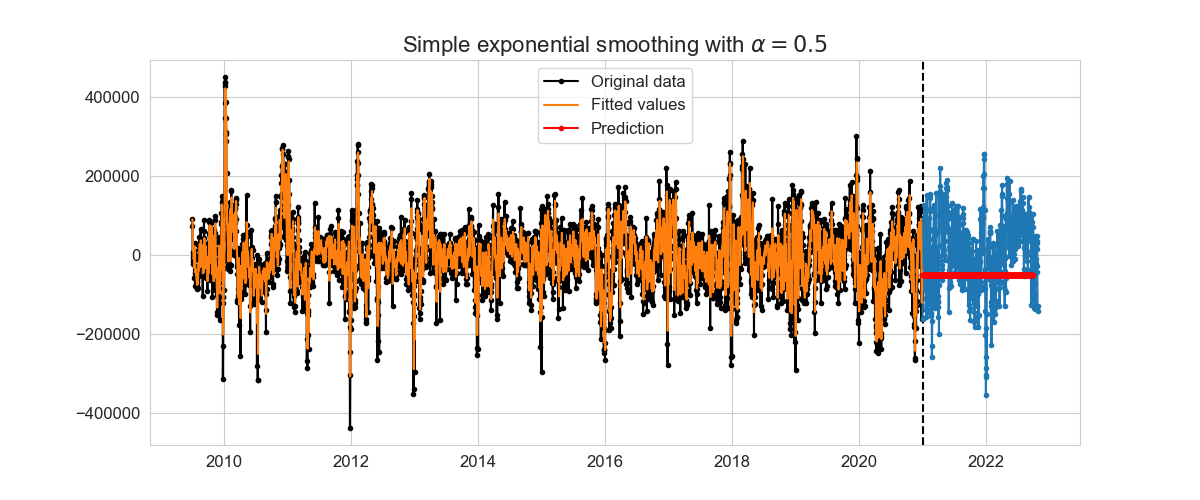
\includegraphics[width = 0.9\textwidth]{imagenes/SimpleES1.png}
    \caption{Valores ajustados y predicción de método de suavizado exponencial simple aplicado a los datos diarios transformados para eliminar los componentes de tendencia y estacionalidad}\label{fig:SimpleES1}
\end{figure}


Los datos disponibles presentan tendencia y efectos estacionales, por tanto, para aplicar este algoritmo, se han eliminado estos componentes. En  la Figura \ref{fig:SimpleES1} se puede ver cómo el modelo ajusta a los datos del conjunto de entrenamiento, mientras que las predicciones son estáticas en el tiempo, con lo que no se ajusta correctamente a los posibles cambios de los datos.

En la Figura \ref{fig:SimpleES2} se presentan tres modelos, en los dos primeros se fija el valor de $\alpha$ como $0.2$ y $0.6$, respectivamente, y el tercer modelo busca el valor óptimo. Se observa en el gráfico que todas las predicciones son estáticas y, además, toma un valor aproximado a la media, $0$. 
\begin{figure}[h]
    \centering
    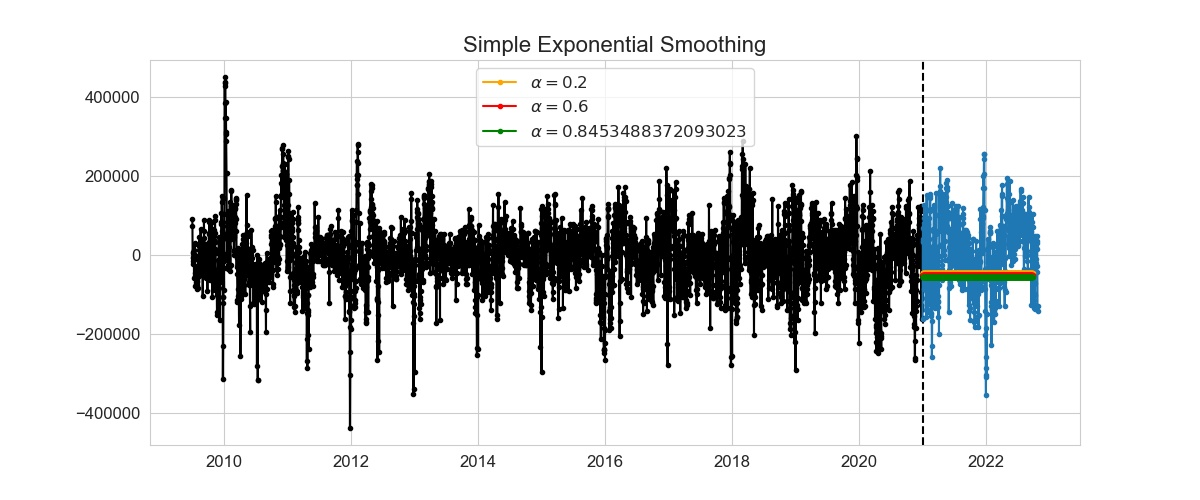
\includegraphics[width = 0.95\textwidth]{imagenes/SimpleES2.jpg}
    \caption{Modelos del método de suavizado exponencial simple con diferentes parámetros de suavizado}\label{fig:SimpleES2}
\end{figure}

\begin{table}[h] 
\centering
\begin{tabular}{cccc} \hline
     & Modelo 1 & Modelo 2 & Modelo 3  \\ \hline
    $\alpha$ &  $0.2$ &   $0.6$ &   $0.005$ \\ 
      % $l_0$ &   $-9935.28$ &  $-9935.28$ &   $-9935.28$ \\ 
      MAPE & $102.09$	 &   $153.66$ &  $99.83$ \\
      MSE  & $2.070\cdot10 ^{9}$ & $2.095\cdot10^{9}$ & $2.070\cdot10^{9}$ \\
      Tiempo (s) & $0.014$ &   $0.0107$ &  $0.0175$ \\ \hline
\end{tabular}
\caption{Parámetros, tiempo y error del método de suavizado exponencial simple} \label{tab:simple_exp}
\end{table}


En la Tabla \ref{tab:simple_exp} se aprecia que el error absoluto medio porcentual asciende hasta el $150\%$. El error alcanza valores tan altos porque los datos son cercanos a cero, es decir, al dividir por dichos valores, el error incrementa rápidamente. Se observa también que el error cuadrático medio se minimiza para los valores de $\alpha=0.2$ y para el valor de $\alpha$ optimizado, como cabe esperar. Sin embargo, el ajuste de las predicciones no es lo suficientemente preciso.



\subsection{Método lineal de Holt}
Charles C. Holt \cite{ES2} extendió el suavizado exponencial simple al suavizado exponencial lineal para permitir el pronósticos con datos que presentan tendencias. También recibe el nombre de método de alisado exponencial doble. La predicción de método lineal de Holt se basa en utilizar dos constantes $\alpha$ y $\beta^*$ (con valores entre $0$ y $1$), y tres ecuaciones
\begin{align}
    \text{Nivel:} \quad& l_t = \alpha X_t + (1-\alpha)(l_{t-1} + b_{t-1}),\label{eq:Holt:nivel}\\
    \text{Crecimiento:} \quad& b_t = \beta^*(l_t - l_{t-1}) + (1-\beta^*)b_{t-1},\label{eq:Holt:crec}\\
    \text{Predicción:} \quad& \hat{X}_{T+h} = l_T + b_Th,\label{eq:Holt:pred}
\end{align}

donde $l_t$ denota una estimación del nivel de la serie en el instante $t$ y $b_t$ denota una estimación de la pendiente (o crecimiento) de la serie en el instante $t$.


La ventaja de este modelo es que puede trabajar con datos con tendencia, por ello, se ha transformado los datos eliminando la componente estacional, para así aplicar este método.

La Figura \ref{fig:Holt1} muestra los valores ajustados y la predicción del modelo lineal de Holt para los valores $\alpha=0.5$ y $\beta^* = 0.0001$. Sin embargo, se observa cómo el valor de la predicción desciende, alejándose de los valores reales.

\begin{figure}[h]
    \centering
    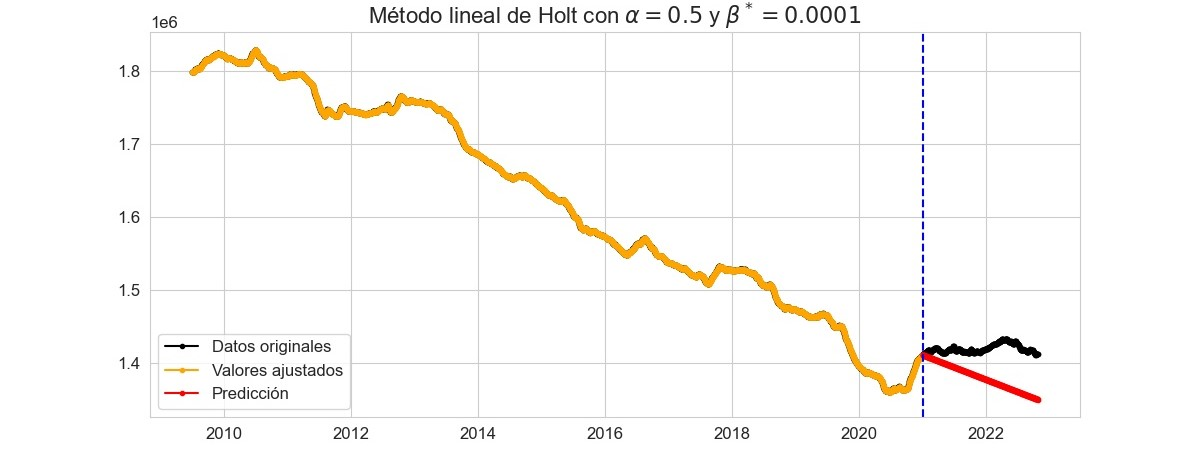
\includegraphics[width = 0.95\textwidth]{imagenes/Holt1.jpg}
    \caption{Valores ajustados y predicción del modelo lineal de Holt aplicado a los datos diarios transformados eliminando el componente estacional}\label{fig:Holt1}
\end{figure}

A continuación se ha probado tres modelos con las opciones disponibles de Python. El primer modelo es el presentado por las ecuaciones \eqref{eq:Holt:nivel}, \eqref{eq:Holt:crec} y \eqref{eq:Holt:pred}. El segundo modelo ajusta la tendencia usando un modelo multiplicativo, en lugar de usar el modelo aditivo visto. Por último, el tercer modelo presenta el método amortiguado del método de Holt, en el cual se introduce un nuevo parámetro de amortiguamiento, $\phi$, por el modelo 
\begin{align*}
    \text{Nivel:} \quad& l_t = \alpha X_t + (1-\alpha)(l_{t-1} + \phi b_{t-1}),\\
    \text{Crecimiento:} \quad& b_t = \beta^*(l_t - l_{t-1}) + (1-\beta^*)\phi b_{t-1},\\
    \text{Predicción:} \quad& \hat{X}_{T+h} = l_T + (\phi + \phi^2 + \dotsb + \phi^h)b_Th.
\end{align*}



Todos los modelos optimizan los valores de $\alpha$ y $\beta^*$, se puede ver los parámetros escogidos en la Tabla \ref{tab:holt}. Los modelos se ejecutan en menos de un segundo, por tanto el tiempo de computación no es un problema en este caso. Sin embargo, en la Figura \ref{fig:Holt2} se observa cómo el modelo aditivo y multiplicativo se aleja de los valores reales del test y no predice correctamente. Los datos presentan una tendencia decreciente a lo largo de los años con ligera subida en los últimos meses del conjunto de entrenamiento, esto provoca que las predicciones con los métodos aditivo y multiplicativo continúen este crecimiento, desviándose de la serie original.
\begin{figure}[h]
    \centering
    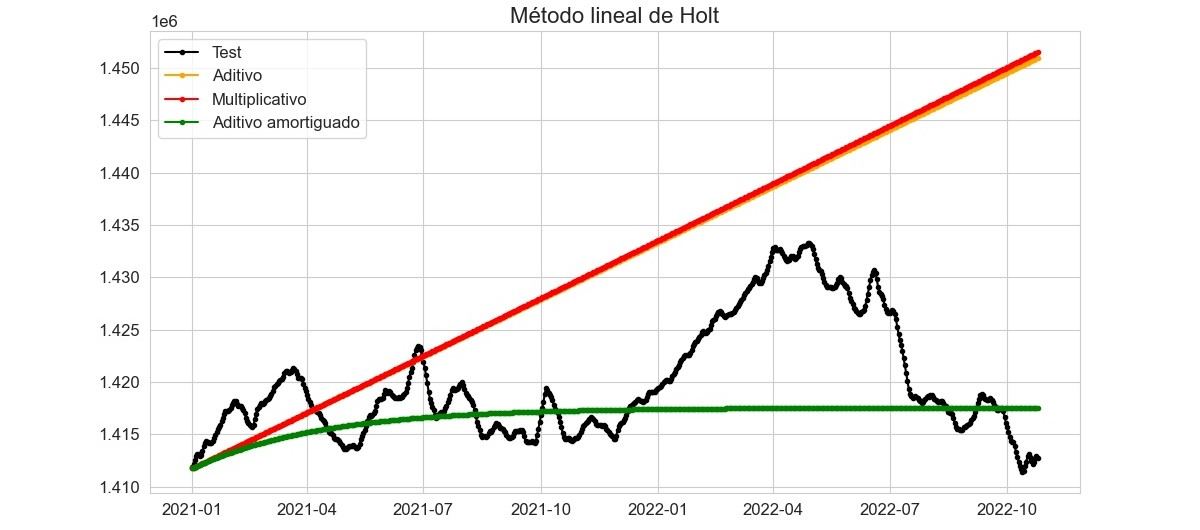
\includegraphics[width = 0.87\textwidth]{imagenes/Holt2.jpg}
    \caption{Predicciones de tres modelos con el método lineal de Holt}\label{fig:Holt2}
\end{figure}

El modelo amortiguado es el único que ofrece una predicción coherente con los datos presentados, aunque a largo plazo las predicciones son estáticas. La Tabla \ref{tab:holt} muestra que los errores MAPE y MSE se minimizan en el modelo amortiguado con valores de $7\%$ y $1.509\cdot10^{10}$, respectivamente.



\begin{table}[ht] 
\centering
\begin{tabular}{cccc}  \hline
     & Aditivo & Multiplicativo & Amortiguado  \\ \hline
    $\alpha$ &  $0.995$ &   $0.995$ &   $0.995$ \\ 
    $\beta$ &  $0.995$ &   $0.995$ &   $0.995$ \\ 
    $\phi$ &  - &   - &   $0.99$ \\ 
    % $l_0$ &   $1847570$ &  $1847570$ &   $1847570$ \\ 
    % $b_0$ &   $39474.44$ &  $39474.44$ &   $39474.44$ \\ 
      MAPE & $23.068$	 &   $22.865$ &  $7.027$ \\
      MSE & $1.390\cdot10^{11}$ & $3.569\cdot10^{10}$ & $1.509\cdot10^{10}$ \\
      Tiempo (s) & $0.171$ &   $0.187$	 &  $0.165$ \\ \hline
\end{tabular}
\caption{Parámetros, error y tiempo del método de Holt } \label{tab:holt}
\end{table}


\newpage
\subsection{Algoritmo de Holt-Winters}
Peter R. Winters \cite{ES3}, discípulo de Holt, extendió el método lineal para incorporar el componente estacional. El método de Holt-Winters consta de tres ecuaciones de suavizado: una para el nivel $l_t$, otra para la tendencia $b_t$ y la última para el componente estacional $s_t$. A cada ecuación le corresponde un parámetro de suavizado $\alpha$, $\beta^*$ y $\gamma$, respectivamente. 
\begin{align*}
    \text{Nivel:} \quad& l_t = \alpha(X_t - s_{t-s}) + (1-\alpha)(l_{t-1} + b_{t-1}),\\
    \text{Crecimiento:} \quad& b_t = \beta^*(l_t - l_{t-1}) + (1-\beta^*)b_{t-1},\\
    \text{Estacionalidad:} \quad& s_t = \gamma (X_t  - l_{t-1} - b_{t-1}) + (1-\gamma)s_{t-s},\\
    \text{Predicción:} \quad& \hat{X}_{T+h} = l_T + b_Th + s_{T+h-s(k+1)},
\end{align*}

donde $s$ es el periodo de estacionalidad y  $k = \lfloor (h-1)/s \rfloor$, lo que asegura que las estimaciones de los índices estacionales utilizados para la predicción provienen del último año de la muestra. También recibe el nombre de método de alisado exponencial triple, por presentar tres ecuaciones de suavizado.

\begin{figure}[h]
    \centering
    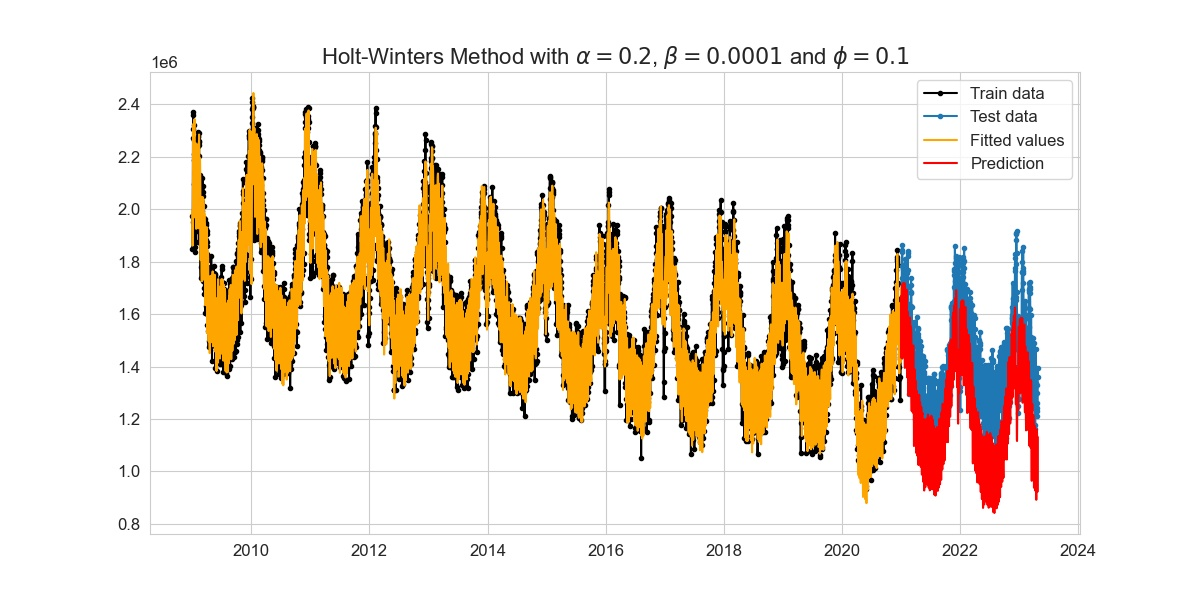
\includegraphics[width = \textwidth]{imagenes/HoltWinters1.jpg}
    \caption{Valores ajustados y predicción del modelo lineal de Holt-Winters}\label{fig:HoltWinters1}
\end{figure}

A continuación, se van a presentar modelos del algoritmo de Holt-Winters aplicados a los datos medidos diariamente y a los datos completos. 

Para los datos medidos diariamente, la Figura \ref{fig:HoltWinters1} muestra cómo el modelo es capaz de ajustarse a los datos del entrenamiento. Sin embargo, en los datos de testeo las predicciones parecen desplazadas hacia abajo. El modelo esperaba que el nivel de la serie siguiera bajando, pero a partir de $2022$ se aprecia una ligera subida, que el modelo no ha sido capaz de predecir.
\begin{table}[h] 
\centering
\begin{tabular}{ccccc}  \hline
     & Aditivo & Multiplicativo & Ad. amortiguado & Mul. Amortiguado  \\ \hline
    $\alpha$ &  $0.6060$ &   $0.995$  &  $0.6060$ &   $0.995$ \\ 
    $\beta$  &  $0.0001$ &   $0.0001$ &  $0.0001$ &  $0.0001$ \\ 
    $\gamma$ &  $0.3939$ & 	 $0.005$  &	 $0.3939$ &   $0.005$ \\
    $\phi$   &     -     &       -    &    $0.99$ &    $0.99$ \\ 
    % $l_0$    & $1798649$ &  $1798649$ & $1798649$ & $1798649$ \\ 
    % $b_0$    &  $177.84$ &  $177.84$ &  $177.84$  &  $177.84$ \\ 
      MAPE   &   $24.13$ &   $17.08$ &   $21.92$  &  $15.75$  \\
      MSE & $1.013\cdot10^{11} $&  $4.105\cdot10^{10}$ & $7.772\cdot10^{10}$ & $3.074\cdot10^{10}$\\
      Tiempo (s) & $2.705$ &   $4.272$	 &  $2.903$ & $4.352$\\ \hline
\end{tabular}
\caption{Parámetros, error y tiempo del método de Holt-WInters} \label{tab:holtwinters}
\end{table}


Al igual que con los otros modelos, se ha implementado las opciones disponibles, ajustado hasta cuatro modelos distintos que aplican el algoritmo de forma aditiva y multiplicativa y a su vez añadiendo o no el parámetro de amortiguamiento. En todos los métodos el algoritmo busca los parámetros óptimos. Los parámetros y resultados se pueden observar en la Tabla \ref{tab:holtwinters}. Se ve que el modelo que minimiza el MAPE y el MSE es el multiplicativo  amortiguado, con un valores de $15\%$ y $3.07\cdot10^{10}$, respectivamente.
\begin{figure}[h]
    \centering
    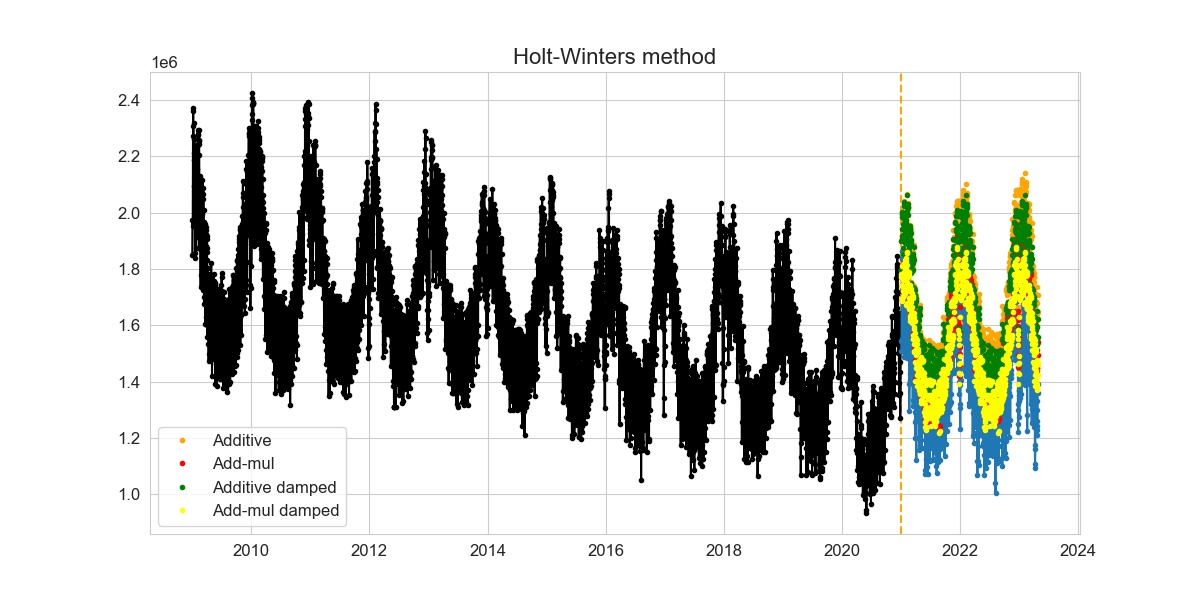
\includegraphics[width = 0.95\textwidth]{imagenes/HoltWinters2.jpg}
    \caption{Predicciones de los cuatro modelos del método de Holt-Winters}\label{fig:HoltWinters2}
\end{figure}

Las predicciones en este caso capturan correctamente el componente estacional que se repite cada año, como se ve en la Figura \ref{fig:HoltWinters2}. Sin embargo, la amplitud de las oscilaciones del conjunto test es mayor que en las predicciones, se ve cómo las predicciones no han sabido capturar los valores más bajos de la serie. No obstante, de forma general, las predicciones sí son buenas con un error del $15\%$. Además, en este caso, el tiempo de computación es de varios segundos, pero si se aumenta el número de datos y el periodo de estacionalidad, este algoritmo puede estar compilando durante horas.




También se ha aplicado este algoritmo al dataset completo, pero como el tiempo de computación era demasiado alto, se ha reducido con conjunto de entrenamiento tomando solamente el último año, 2020. De este modo, se ha intentado modelar la estacionalidad mensual que presentan los datos. En la Figura \ref{fig:HoltWinters4} se observa cómo el algoritmo sí se adapta a los datos del conjunto de entrenamiento, sin embargo su actuación en el conjunto de testeo es muy deficiente.
\begin{figure}[h]
    \centering
    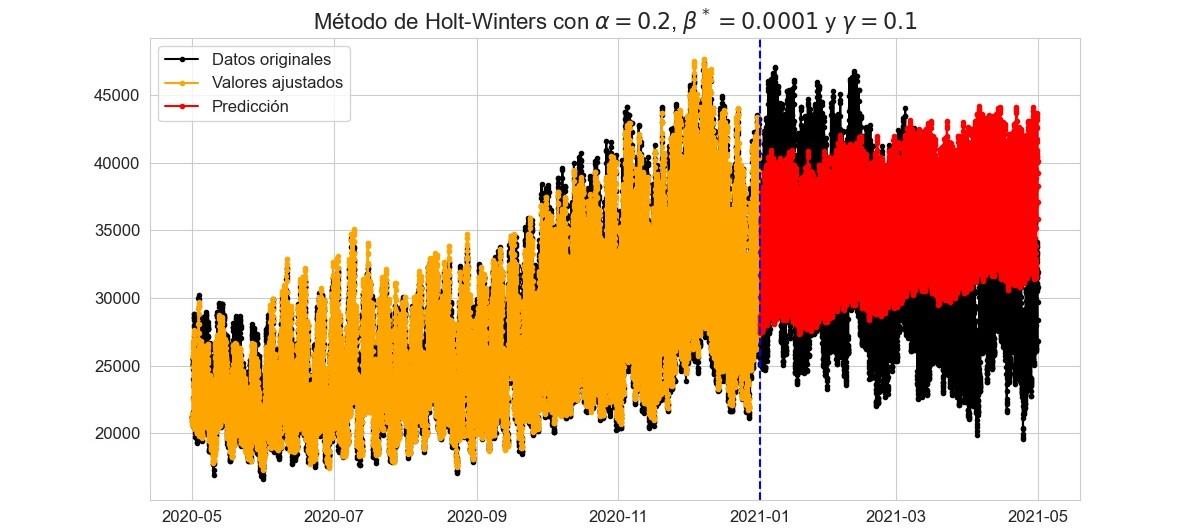
\includegraphics[width = 0.95\textwidth]{imagenes/HoltWinters4.jpg}
    \caption{Predicciones del método de Holt-Winters para los datos compeltos}\label{fig:HoltWinters4}
\end{figure}

En cuanto a las predicciones, este método no modela correctamente la estacionalidad presente en los datos. Además, en cuanto a la tendencia, se ve que en el train hay cierto crecimiento que provoca que en las predicciones también también asciendan con el paso del tiempo, mientras que los valores reales descienden. También cabe resaltar la amplitud de las oscilaciones de la predicción, que son menores a los valores reales. De este modo, se ve que no logra ajustar a los valores más extremos que presenta la serie. En este caso el tiempo de computación es de $3$ minutos y $43$ segundos y el MAPE es $23.63\%$.



El algoritmo funciona correctamente modelando los datos diarios, sin embargo aún no se ha encontrado un método de series temporales clásico o de alisado exponencial que permita ajustar a los datos completos. Por ello, en las próximas secciones se presentarán nuevos métodos que conseguirán cumplir dicho objetivo.









\newpage
\section{Prophet}
Prophet es un software de código abierto que fue desarrollado internamente en \emph{Facebook} (ahora conocido como \emph{Meta}), por Sean J. Taylor y Ben Lethan \cite{Prophet1}, para afrontar dos de los problemas más comunes en las metodologías de predicción:
\begin{enumerate}
    \item Las herramientas de predicción más automáticas disponibles tienden a ser inflexibles e incapaces de ajustarse a suposiciones adicionales.
    \item La herramientas de predicción más robustas requieren un analista especializado en la ciencia de datos.
\end{enumerate}

Facebook experimentó demasiada demanda de pronósticos de alta calidad, la cual los analistas no podían proporcionar. En 2017, Facebook lanzó Prophet al público como software de código abierto para solventar este problema.

El modelo de Prophet consiste en usar un modelo descomponible de series temporales que tiene en cuenta tres factores importantes: la tendencia, la estacionalidad y los días festivos. Estos componentes son combinados en la ecuación
\begin{equation}\label{eq:prophet:descom}
    y(t) = g(t) + s(t) + h(t) + \varepsilon_t .
\end{equation}
El valor de $y$ pronosticado por el modelo en el momento $t$ viene dado por la función $y(t)$ y se descompone en cuatro sumandos:
\begin{itemize}
    \item $g(t)$ se corresponde con la componente de crecimiento o la tendencia general, que modela los cambios no periódicos.
    \item $s(t)$ representa la componente estacional, que es la suma de todos los componentes periódicos.
    \item $h(t)$ representa los efectos de los días festivos, que ocurre en calendarios irregulares durante uno o más días.
    \item $\varepsilon_t$ es el término del error, que engloba todos los demás cambios que no ajustan los demás componentes del modelo.
\end{itemize}

La combinación de estos componentes es todo lo que Prophet requiere para construir las predicciones. Para comprender cómo funciona Prophet es necesario desglosar y estudiar cada uno de estos componentes.

La implemtación de Python se hace a través del paquete \texttt{fbprophet} (o \texttt{prophet}) y la función que permite ajustar el modelo es \texttt{Prophet} \cite{Prophet2}.

\subsection{Modelos de tendencia}
Con el fin de ajustar el componente de tendencias se implementan dos tipos de modelo: un modelo lineal y un modelo logístico. Para pronosticar problemas que no muestran una tendencia convergente, el modelo lineal se escribe como
\begin{equation} \label{eq:prophet:g_lineal}
    g(t) = (k+\mathbf{a}(t)^T \boldsymbol{\delta})t + (m + \mathbf{a}(t)^T\boldsymbol{\gamma}).
\end{equation}
Este es un modelo lineal definido a trozos, es decir, la pendiente cambia como una función de $t$. Por ello, a la pendiente $k$ se le añade $\mathbf{a}(t)^T\boldsymbol{\delta}$, donde la variable $k$ es la tasa de crecimiento. 

Se modela que existe $S$ puntos de cambio en los tiempos $s_j$, $j=1,\dotsc, S$, donde la tasa de crecimiento puede cambiar. Se define el vector de ajustes de tasa $\boldsymbol{\delta}\in \mathbb{R}^S$, donde $\delta_j$ es el cambio en la tasa que ocurre en el tiempo $s_j$. De esta forma, para cualquier tiempo $t$ la tasa es la suma de una tasa base $k$ con todos los ajustes que ocurren hasta este tiempo, es decir, $k + \sum_{j: t>s_j} \delta_j$. Para representarlo de forma más compacta se define el vector $\mathbf{a}(t)\in \{0, 1\}^S$ tal que
\begin{equation*}
    a_j(t) = \left\{ \begin{array}{ll}
        1, & \text{si } t\geq s_j,  \\
        0, & \text{en otro caso.}
    \end{array}\right.
\end{equation*}
De este modo, el crecimiento para un tiempo dado $t$ es $k + \mathbf{a}(t)^T \boldsymbol{\delta}$. En la implementación de Python, por defecto se considera $25$ cambios de tendencia (con el parámetro \texttt{n\_changepoints} se puede especificar este número) uniformemente distribuido a los largo del primer $80\%$ de la serie. No ajusta el restante $20\%$ para evitar sobre ajustes al final de la serie. Es posible ampliar o reducir este rango con el parámetro \texttt{changepoint\_range}.

Por último, para que la curva sea continua, es necesario ajustar los segmentos entre cada punto de cambio. Al igual que con la pendiente, el parámetro de compensación es una variable base $m$ añadiendo todos los cambios hasta el tiempo $t$, es decir, $m + \mathbf{a}(t)^T\boldsymbol{\gamma}$, donde $\boldsymbol{\gamma}$ es el vector de ajustes de compensación. En este modelo, con el fin de que la curva sea continua, $\boldsymbol{\gamma}$ se toma de forma que $\gamma_j = - s_j\delta_j$. 

El valor del parámetro $m$ se puede interpretar como el valor base de la tendencia. Para el instante $0$, el valor de la tendencia es $m$ y según avanza el tiempo este valor cambia en los puntos de cambio para ajustarse a la variaciones de la serie.

La Figura \ref{fig:changepoints} muestra un modelo de tendencia lineal con puntos de cambio ajustados a los datos.
\begin{figure}[h]
\centering
    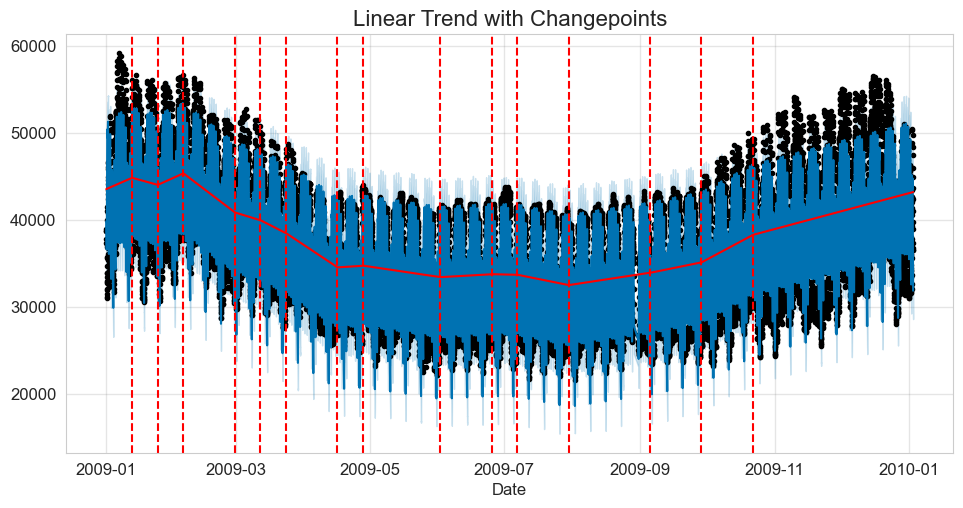
\includegraphics[width =0.85\textwidth]{imagenes/changepoints.png}
    \caption{Modelo de tendencia lineal con puntos de cambio}\label{fig:changepoints}
\end{figure}

Por otro lado, para series temporales que sí presentan una tendencia convergente, es importante modelar cómo ha crecido la serie y cómo se espera que siga creciendo. En este caso se emplea un modelo de crecimiento logístico, dado por la ecuación
\begin{equation}\label{eq:prophet:g_log}
    g(t) = \frac{C}{1 + \exp{(-k(t-m))}},
\end{equation}
donde $C$ es la cota máxima de los datos, $k$ la tasa de crecimiento y $m$ un parámetro de compensación. 

El modelo presentado en \eqref{eq:prophet:g_log} tiene sus limitaciones. Primeramente, la cota máxima no es siempre constante, por tanto es necesario introducir una función $C(t)$ que represente esta cota a lo largo del tiempo. Por otra parte, al igual que en el modelo anterior, se plantea la tasa de crecimiento como $k + \mathbf{a}(t)^T\boldsymbol{\delta}$ y el parámetro de compensación como $m + \mathbf{a}(t)^t\boldsymbol{\gamma}$ y, con el fin de conectar correctamente los extremos de los segmentos, se cambia los valores de $\gamma_j$, $j=1,\dotsc,S$. En este modelo, se tiene que 
\begin{equation}
    \gamma_j = \left(s_j-m-\sum_{l<j}\gamma_l\right)\left(1 - \frac{k+\sum_{l<j}\delta_l}{k+\sum_{l\leq j}\delta_l}\right).
\end{equation}
El modelo de crecimiento logístico por partes es 
\begin{equation}\label{eq:prophet:g_log2}
     g(t) = \frac{C(t)}{1 + \exp{(-(k+\mathbf{a}(t)^T\boldsymbol{\delta})(t-(m+\mathbf{a}(t)^T\boldsymbol{\gamma}))}}.
\end{equation}

También se puede especificar el número de puntos de cambio. Se supone $\delta_j \sim \text{Laplace}(0, \tau)$, donde $\tau$ controla la flexibilidad del modelo para alterar su tasa. Según el valor de $\tau$ se acerca a $0$, el ajuste se reduce al crecimiento lineal o logístico estándar, es decir, no es función definida por partes.

En la implementación de Python este parámetro es conocido como \texttt{changepoint\_prior \_scale}, con un valor predeterminado de $0.05$. Aumentar este valor significa que todos los puntos de cambio tendrán mayor influencia en el modelo, incluso si son cambios pequeños. Permite que el modelo sea flexible y sensible a cambios de tendencia.

Si el valor es cercano a $0$, los puntos de cambio de tendencia tendrán una menor influencia en el modelo. En este caso, el modelo será más rígido y menos propenso a ajustar cambios en la tendencia.

Los parámetros $k$ y $m$ se escogen buscando la combinación que minimice el error cuadrático medio para el conjunto de entrenamiento. Este proceso lo realiza Python internamente a través de la función \texttt{Prophet}.

Además, el parámetro \texttt{growth} permite especificar el tipo de tendencia que del modelo, con las opciones de modelo de tendencia lineal, logístico o plano, este último es para datos que no presentan ningún tipo de crecimiento, donde $g(t)$ es nula.





\subsection{Estacionalidad}
Los datos de series temporales a menudo exhiben periodicidad, especialmente con datos comerciales, donde a menudo hay ciclos anuales, semanales y diarios. Prophet puede modelar un número ilimitado de dichos componentes periódicos en su término de estacionalidad, $s(t)$, de la ecuación \eqref{eq:prophet:descom}.

Prophet se basa en las series de Fourier para ajustar el componente estacional. Sea $P$ el periodo regular que se espera en la serie temporal, los efectos estacionales se aproximan mediante la fórmula
\begin{equation}\label{eq:prophet:s}
    s(t) = \sum_{n=1}^N \left( a_n\cos{\left(\frac{2\pi n t}{P}\right)} + b_n \sin{\left(\frac{2 \pi n t}{P}\right)}\right),
\end{equation}
que consiste en una serie de Fourier estándar. En este caso no se considera el término independiente porque a su vez también se ajusta el componente de tendencia.

\begin{figure}[h]
\centering
    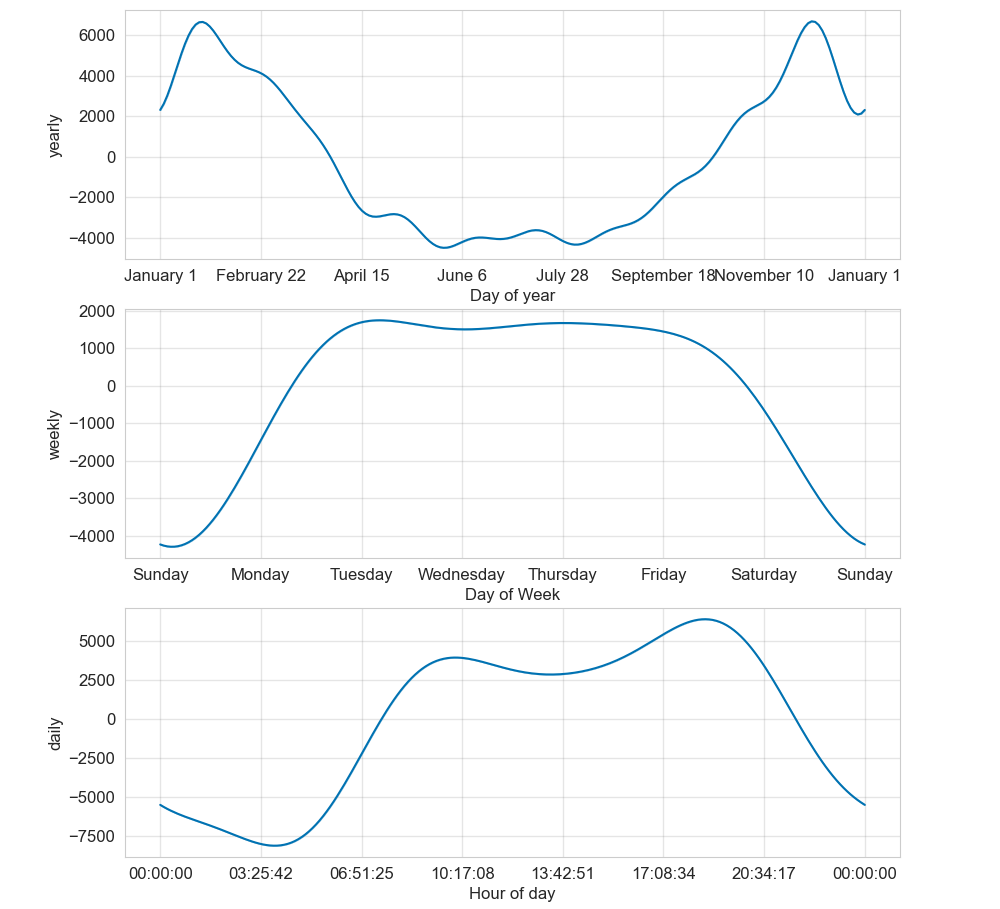
\includegraphics[width = 0.95\textwidth]{imagenes/prophet_comp.png}
    \caption{Componentes de estacionalidad del modelo Prophet}\label{fig:prophet_comp}
\end{figure}


Ajustar el modelo \eqref{eq:prophet:s} a los datos requiere estimar un total de $2N$ parámetros, $\boldsymbol{\beta} = [a_1, b_1, \dotsc, a_N, b_N]^T$. Esta estimación se hace a partir de una matriz de estacionalidad con los vectores para cada valor de $t$ de los datos históricos y los datos futuros. Por ejemplo, para estacionalidad semanal y $N=3$, 
\begin{equation*}
    X(t) = \left[ \cos{\left(\frac{2\pi (1)t}{7}\right)} , \sin{\left( \frac{2\pi(1)t}{7}\right)},  \dotsc, \sin{\left( \frac{2\pi(3)t}{7}\right)}  \right].
\end{equation*}
El componente estacional es
\begin{equation}\label{eq:prophet:s2}
    s(t) = X(t) \boldsymbol{\beta}.
\end{equation}



En este modelo generativo se toma $\boldsymbol{\beta} \sim \text{Normal}(0, \sigma^2)$ para imponer un suavizado previo a la estacionalidad. Aumentar $N$ permite ajustar los patrones de los datos que cambian rápidamente, sin embargo este aumento también incrementa el riesgo de sobreajustar el modelo. Para datos con patrones anuales y semanales se ha visto que $N=10$ y $N=3$, respectivamente, funciona correctamente para la mayoría de los problemas. La obtención de estos parámetros se puede automatizar usando un procedimiento de selección del modelo, como puede ser el criterio AIC (criterio de información de Akaike).

Utilizar las series de Fourier es muy práctico a la hora de ajustar los diferentes periodos de estacionalidad. En la Figura \ref{fig:prophet_comp} puede observarse cómo se modelan los componentes anual, semanal y diario de los datos. Se puede ver que, en los meses centrales del año, la demanda eléctrica alcanza el mínimo. Por otro lado, los días de la semana con menor demanda son sábado y domingo y las horas del día con menor demanda es durante las horas de la madrugada.

La implementación en Python permite indicar al modelo el parámetro $\boldsymbol{\beta}$ (con el parámetro \texttt{seasonality\_prior\_scale}) para modelar la influencia de los efectos estacionales en el modelo. Además, se puede especificar el tipo de estacionalidad (aditiva o multiplicativa) con el parámetro \texttt{seasonality\_mode}, por defecto Prophet trabaja con modelos aditivos. 

En el caso ajustar el tipo de modelo como \texttt{seasonality\_mode=`multiplicative'}, Prophet utiliza un modelo multiplicativo tanto para el componente estacional como a los efectos de la vacaciones u otros regresores (variables exógenas), pero es posible especificar el modo de cada componente mediante el parámetro \texttt{mode}. Para el modelo multiplicativo se considera las mismas fórmulas combinadas multiplicativamente en lugar de aditivamente.



\subsection{Días festivos y eventos}
Los componentes del modelo Prophet presentados hasta ahora se corresponden con las de la descomposición clásica de la serie temporal. Los analistas de \emph{Facebook} decidieron añadir también un nuevo componente, que modela los efectos de los días festivos, ya que las vacaciones pueden provocar alteraciones en las actividades de negocios. 

\begin{table}[h] 
\centering
\begin{tabular}{cc} \hline
Holiday & Date \\\hline
New Year's Day & 01-01-2009\\
New Year's Day & 01-01-2010\\
Good Friday & 10-04-2009 \\
Good Friday & 02-04-2010 \\
Good Friday & 22-04-2011 \\ \hline

\end{tabular}
\caption{Días festivos en Reino Unido} \label{tab:festivos}
\end{table}
La incorporación de una lista de días festivos en el modelo se simplifica asumiendo que los efectos de los días festivos son independientes. Para cada día festivo $i$, sea $D_i$ el conjunto de las fechas pasadas y futuras de dicho festivo, la Tabla \ref{tab:festivos} exhibe un ejemplo de cómo se introduce la información de las vacaciones en Python. Se añade una función indicadora que represente si un tiempo $t$ es durante el festivo $i$, y se le asigna a cada vacación el parámetro $\kappa_i$, que es el cambio en la predicción. Se crea una matriz de regresión
\begin{equation*}
    Z(t) = [\mathbf{1}(t\in D_1), \dotsc, \mathbf{1}(t\in D_L)]
\end{equation*}
y se toma 
\begin{equation}\label{eq:prophet:h}
    h(t) = Z(t) \boldsymbol{\kappa}.
    \end{equation}

Al igual que con la estacionalidad, se considera que a priori $\boldsymbol{\kappa} \sim \text{Normal}(0, \nu^2)$. A menudo es importante añadir los efectos de los días festivos en un umbral alrededor de los mismos. Para ello se incluyen parámetros adicionales para los días circundantes a los festivos, tratando estos días como festivos. La Figura \ref{fig:prophet_hday} es un gráfico con los efectos de las vacaciones en el modelo, se observa que para los días festivos la demanda eléctrica tiende a disminuir.
\begin{figure}[h]
\centering
    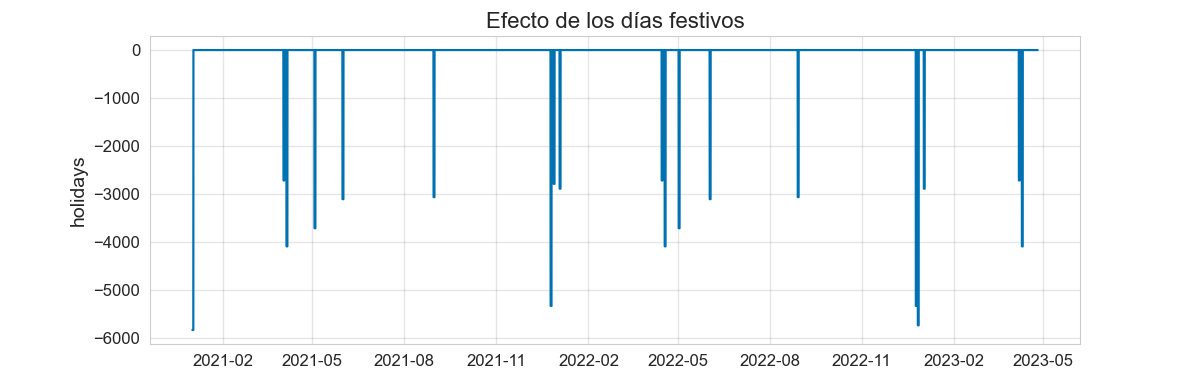
\includegraphics[width = 0.9\textwidth]{imagenes/prophet_hday.png}
    \caption{Efecto de los días festivos en los datos}\label{fig:prophet_hday}
\end{figure}


La implementación en Python permite indicar al modelo la lista de fechas (mediante el parámetro \texttt{holidays}) y el parámetro $\boldsymbol{\kappa}$ (\texttt{holidays\_prior\_scale}) modela la influencia de dichos factores en el modelo. Este parámetro puede ser global o ser definido individualmente para cada fecha.

Otro parámetro que cabe destacar en la documentación de \texttt{Prophet} es el atributo \texttt{add\_regressor}. Este parámetro permite añadir variables exógenas al modelo. La forma de implementarlo es igual al explicado en la Sección \ref{sec:SARIMA} para el proceso SARIMA, en este caso se utiliza el modelo Prophet para predecir los valores de la variable exógena. 



\subsection{Prediciones con Prophet}
En esta sección se va a estudiar la actuación del modelo presentado aplicado a los datos que se dispone.  Una vez ajustados todos los componentes de la ecuación \eqref{eq:prophet:descom} el algoritmo se encarga de hacer las predicciones para cualquier valor de $t$.

Los componentes que modelan la estacionalidad y las vacaciones vistos se aplican al modelo sin ningún cambio. Sin embargo, la predicción de la tendencia es diferente, si el modelo se extrapola al futuro entonces la tendencia tendría una tasa constante. 

Para el componente de tendencia se modela que hay $S$ puntos de cambio en el conjunto entrenamiento. De este mismo modo, se proponen futuros puntos de cambio dispuestos de forma aleatoria y de forma que la frecuencia media de los puntos de cambio coincide con
\begin{equation*}
    \left\{\begin{array}{l}
        \delta_j = 0 \text{  con probabilidad  } \frac{T-S}{S,}  \\
         \delta_j \sim \text{Laplace}(0, \lambda) \text{  con probabilidad 
 } \frac{S}{T} ,
    \end{array}\right. \quad \forall j > T,
\end{equation*}
donde $\lambda$ se puede estimar con la estimación de máxima verosimilitud, es decir, $\lambda = \frac{1}{S} \sum_{j=1}^S \abs{\delta_j}$. Así, se asume que la tendencia continúa presentando cambios con la misma frecuencia y magnitud que la que ha tenido en el conjunto de entrenamiento. 


\begin{figure}[h]
\centering
    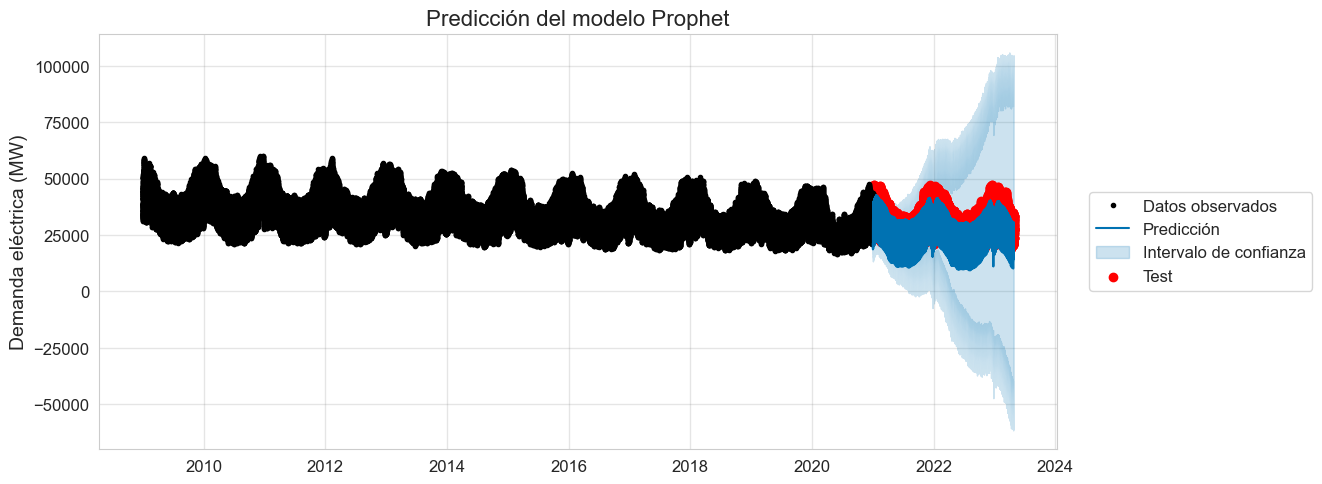
\includegraphics[width = \textwidth]{imagenes/prophet_predition.png}
    \caption{Predicciones con el modelo Prophet}\label{fig:prophet_predition}
\end{figure}

El algoritmo de Prophet es capaz de modelar los datos teniendo en cuenta los diferentes tipos de estacionalidad que otros modelos no han podido manejar. La Figura \ref{fig:prophet_predition} muestra las predicciones del modelo Prophet con los parámetros por defecto. 
\begin{figure}[h]
\centering
    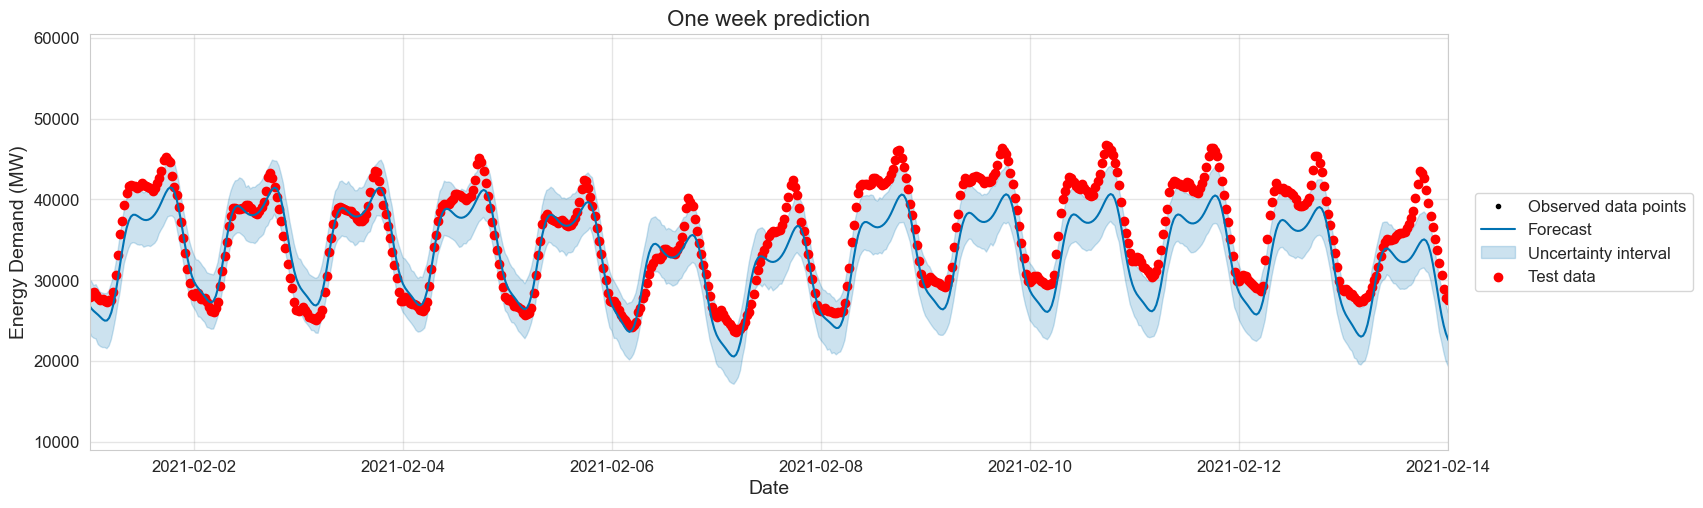
\includegraphics[width = 0.85\textwidth]{imagenes/prophet_oneweek_pred.png}
    \caption{Predicciones con el modelo Prophet para una semana aleatoria}\label{fig:prophet_oneweek_pred}
\end{figure}


Al fijarse en una semana aleatoria, Figura \ref{fig:prophet_oneweek_pred}, se ve cómo este algoritmo sí ha sabido adaptarse a las variaciones de los datos durante un día. En este caso el tiempo de computación es de $19$ minutos. No es un algoritmo que se ejecute de forma inmediata, pero dada la magnitud de los datos y la precisión del modelo, es un tiempo razonable. En este caso, el MAPE es del $11.88\%$, siendo hasta el momento el modelo capaz de adaptar los datos con menor error.


A continuación, se ha implementado el mismo modelo, pero añadiendo también los efectos de los días festivos. Como se ha visto, por lo general en este dataset los días festivos provocan que haya un descenso en el consumo eléctrico. 
\begin{figure}[h]
\centering
    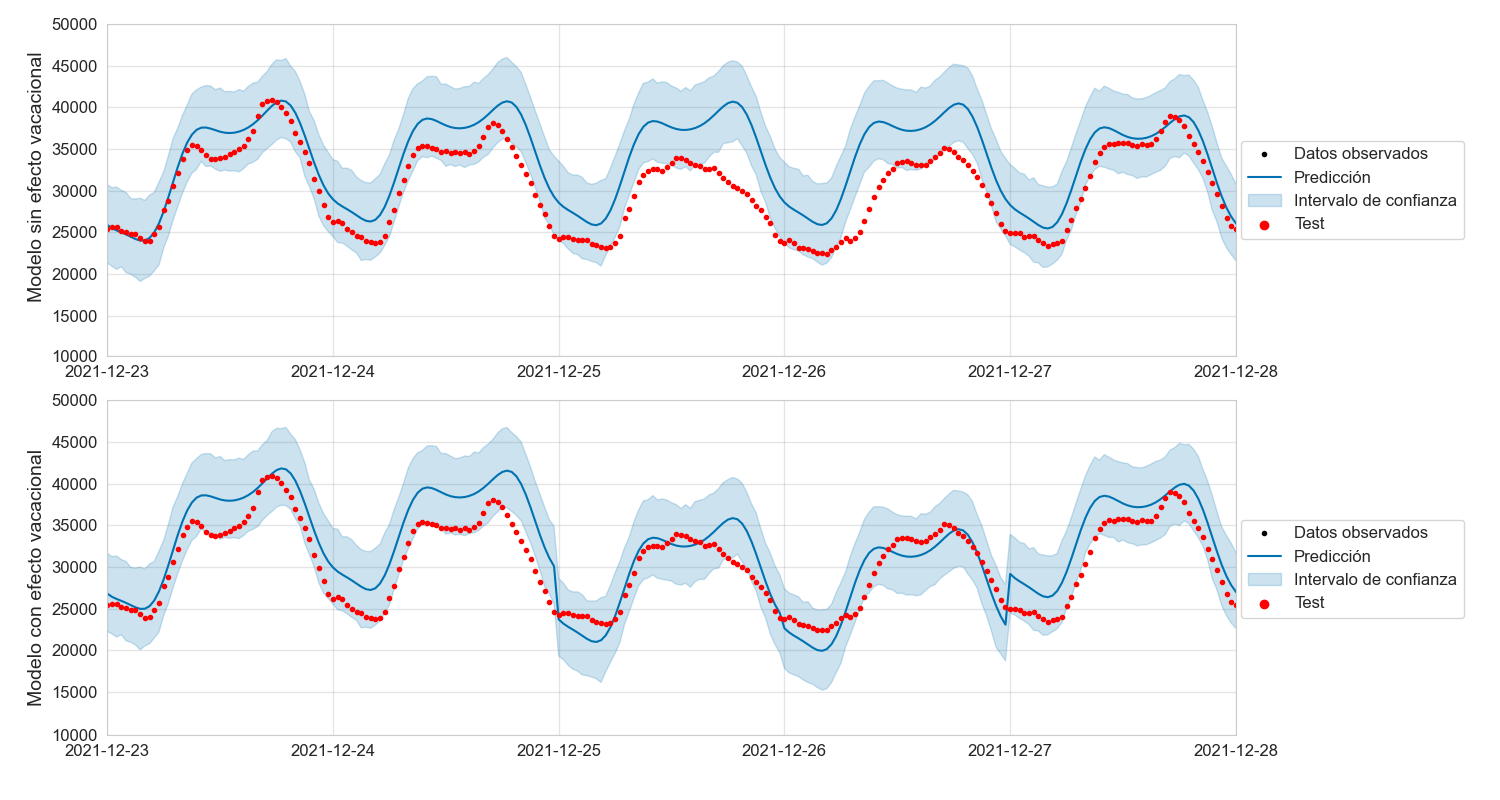
\includegraphics[width = 0.8
    \textwidth]{imagenes/prophet_hdaycomparison.png}
    \caption{Comparación de modelos con y sin efecto vacacional}\label{fig:prophet_hdaycomparison}
\end{figure}

Se puede comparar el modelo con el componente vacacional y el primer modelo, observado la Figura \ref{fig:prophet_hdaycomparison}. El segundo modelo se ajusta de forma más precisa, pues en el primer modelos, los valores reales ni siquiera caen en el intervalo de confianza del $95\%$ para los días $26$ y $27$ de diciembre.

En este caso, el algoritmo ha tardado $23$ minutos y el error es $11.86\%$. El error no ha mejorado significativamente respecto al anterior, pero sí ha ajustado correctamente los posibles efectos vacacionales.
\begin{figure}[h]
\centering
    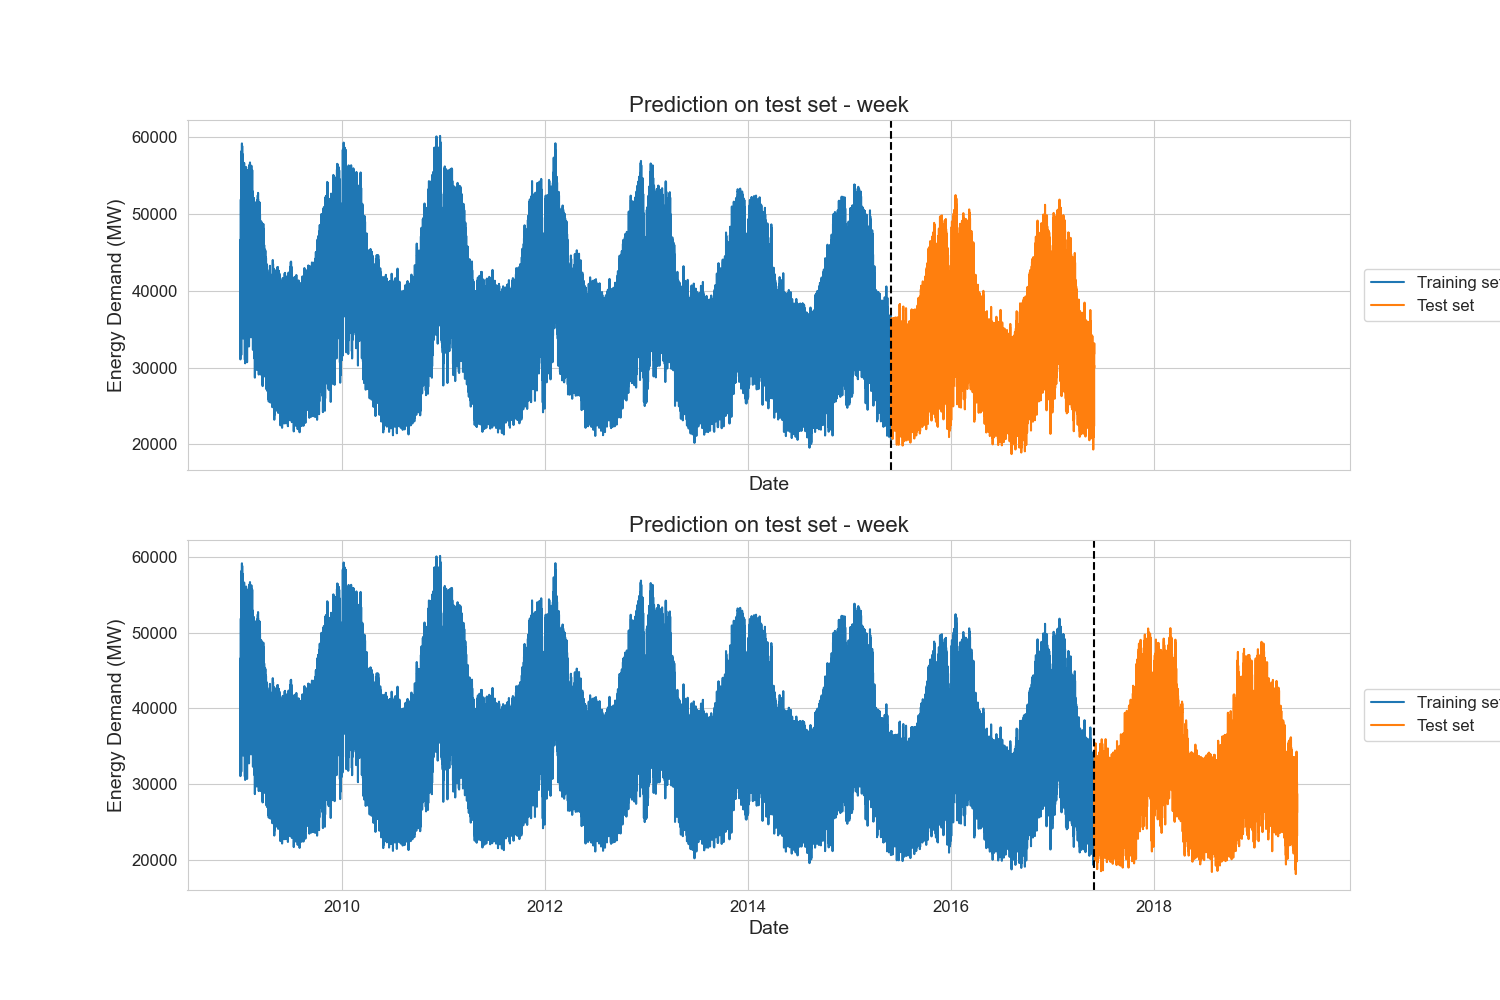
\includegraphics[width = 0.85\textwidth]{imagenes/prophet_crossval.png}
    \caption{Separación de los datos para validación cruzada}\label{fig:prophet_crossval}
\end{figure}


El último modelo que se propone es resultado de aplicar validación cruzada a los datos, la Figura \ref{fig:prophet_crossval} muestra esta división. Se ha tomado solamente dos divisiones para que el tiempo de computación no ascienda demasiado a la hora de buscar los parámetros.


\begin{table}[h]
    \centering
    \begin{tabular}{ccc} \hline
         changepoint\_prior\_scale ($\tau$) & seasonality\_prior\_scale ($\sigma^2$) & holidays\_prior\_scale ($\nu^2$) \\ \hline
         0.001 & 2.5 & 10 \\ \hline
    \end{tabular}
    \caption{Parámetros obtenidos con validación cruzada}
    \label{tab:param_crossval}
\end{table}


En este caso lo parámetros que se ha intentado optimizar son \texttt{changepoint\_prior\_scale},  \texttt{seasonality\_prior\_scale} y \texttt{holidays\_prior\_scale}. Los resultados de la validación cruzada se encuentran en la Tabla \ref{tab:param_crossval}. En Python, los valores predeterminados de estas variables son $\tau = 0.05$, $\sigma^2 = 10$ y $\nu^2 = 10$, a partir de estos valores se va a interpretar los obtenidos. Respecto a los puntos de cambios, se ha tomado un valor pequeño, es decir permite poco cambios de tendencia. De esta forma también se evita el sobreajuste del modelo, se ha reducido el número de puntos de cambio de $25$ a $8$, como muestra la Figura \ref{fig:changepoints2}.
\begin{figure}[h]
\centering
    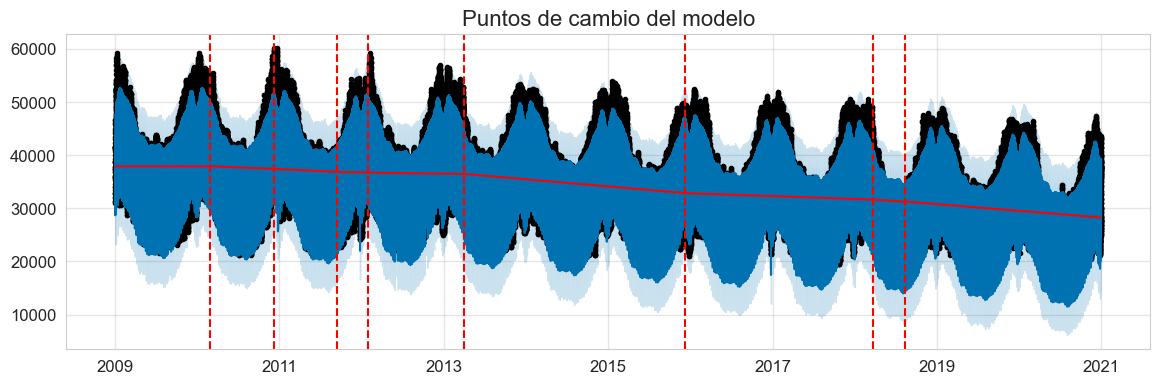
\includegraphics[width =0.85\textwidth]{imagenes/changepoints2.png}
    \caption{Puntos de cambio en el nuevo modelo}\label{fig:changepoints2}
\end{figure}



Se ha visto que la tendencia de este modelo no varía significativamente e incluso puede modelarse con un recta. Teniendo en cuenta la estacionalidad, el modelo toma un valor menor al fijado, en otras palabras, es conveniente no darle tanto peso a los cambios estacionales. 


Por último, respecto al componente que modela los días festivos, la validación cruzada ha dado el mismo valor que el fijado por Python, es decir, este valor es suficiente para ajustar los datos en los días festivos.
\begin{figure}[h]
\centering
    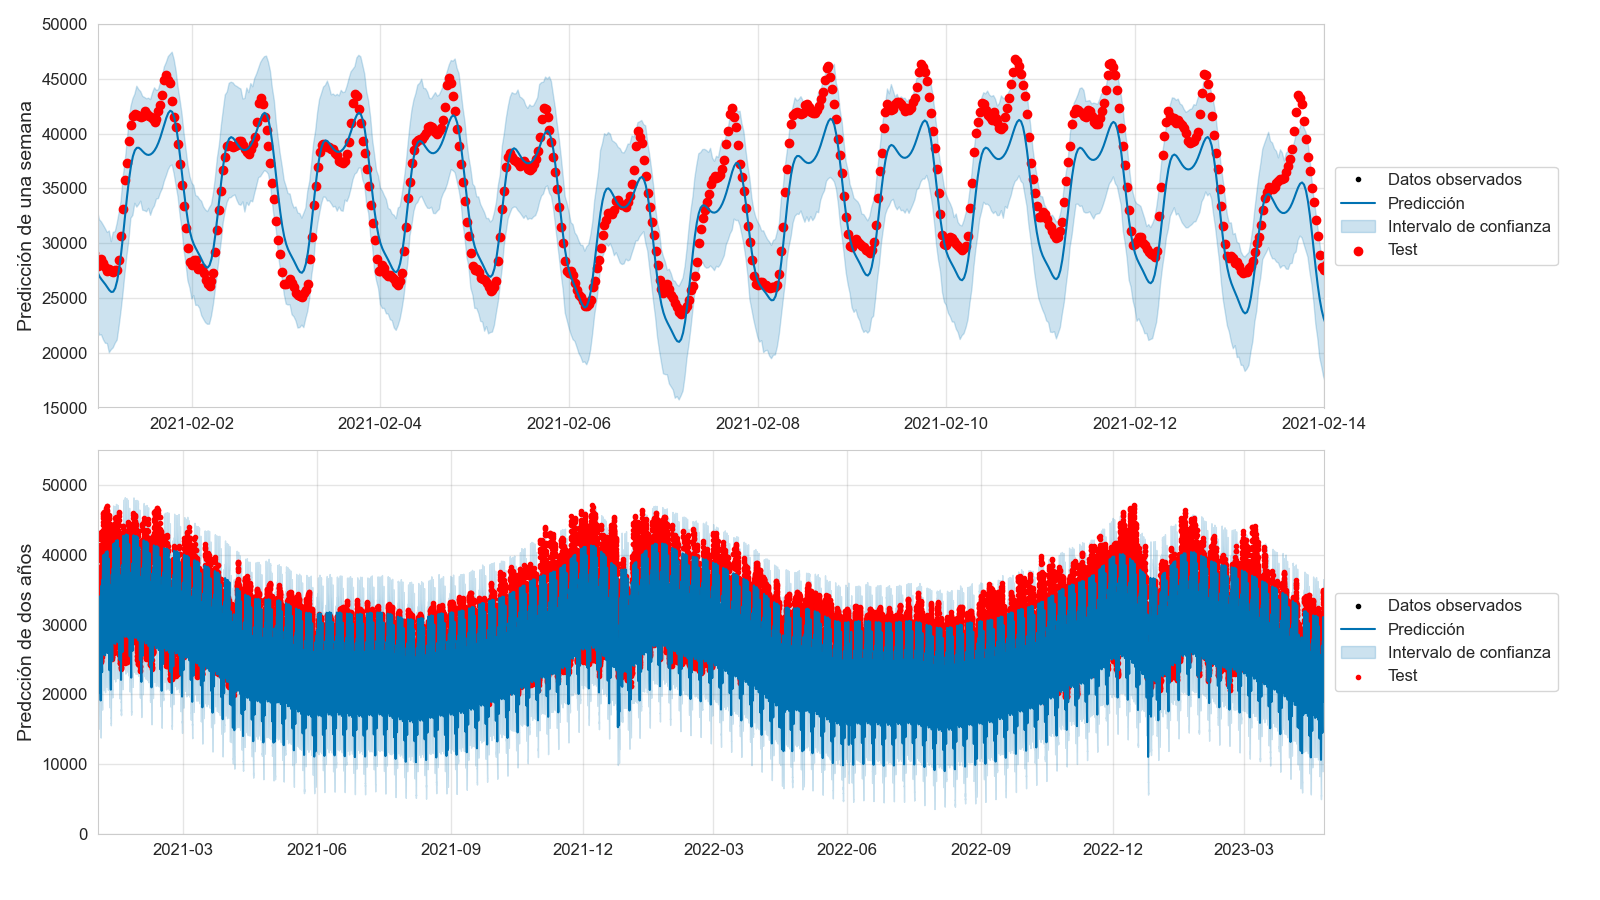
\includegraphics[width =0.83\textwidth]{imagenes/prophet_pred2.png}
    \caption{Predicciones del modelo optimizado}\label{fig:prophet_pred2}
\end{figure}


En la Figura \ref{fig:prophet_pred2} se observa la actuación del modelo con los parámetros escogidos. La primera gráfica muestra dos semanas aleatorias del conjunto de testeo, las dos primeras semanas de febrero de 2021. Se ve cómo el modelo consigue ajustar a los cambios horarios que ocurren durante el día, además de las fluctuaciones que ocurren a lo largo de la semana. Por ejemplo, se observa una baja en el día 7 que sigue de una subida los siguientes días y el modelo es capaz de capturar esos cambios.

La segunda gráfica muestra las predicciones de todo el conjunto test. Se ve cómo el modelo ajusta los cambios estacionales anuales, que presentan un pico durante las vacaciones de navidad. El modelo se adapta correctamente, pero no predice los valores más altos de la serie, ya que predice una bajada de la tendencia. Se puede ver cómo también el intervalo de confianza aumenta rápidamente a la vez que las predicciones son más futuras.
\begin{table}[h]
    \centering
    \begin{tabular}{ccc} \hline
        MAPE & MSE & Tiempo \\ \hline
        $11.83\%$ & $1.740\cdot10^7$ &  $418$ \\\hline
    \end{tabular}
    \caption{Errores y tiempo del modelo Prophet optimizado}
    \label{tab:Prophet_error}
\end{table}


El error absoluto medio porcentual final de este modelo es de $11.83$, ha mejorado respecto a los otros en un $0.06\%$, y el tiempo de ejecución es de $6$ minutos y $58$ segundos.

















\newpage
\section{Modelos autorregresivos con árboles de decisión}
Los CART (\emph{Classification and Regression Tree}) \cite{DT1} son modelos de aprendizaje automático y una técnica de análisis predictivo que se utiliza para tomar decisiones o predecir resultados. Su efectividad y su facilidad para representarlos gráficamente han hecho de los árboles de decisión unos de los algoritmos más populares en Machine Learning.

El proceso de construcción de un CART comienza con un nodo raíz que contiene todo el conjunto de datos. A continuación, se evalúa una característica de los datos y se divide en dos o más subconjuntos, utilizando un criterio de división, este criterio de división puede ser un método que busque maximizar la pureza de los subconjuntos. Una vez que se realiza la división, se crean nodos hijos correspondientes a cada subconjunto y se repite el proceso de forma recursiva en cada uno de ellos. Esta recursión continúa hasta que se cumple algún criterio de parada, como puede ser alcanzar un número máximo de profundidad o un número mínimo de observaciones por hoja.

En el caso de un problema de clasificación, cada hoja del árbol representa una clase, y se le asigna la clase con mayor presencia en esa hoja. Por otro lado, para problemas de regresión, cada hoja representa un valor numérico que se estima como la media de los valores de la variable en esa hoja.


\begin{figure}[h]
\centering
    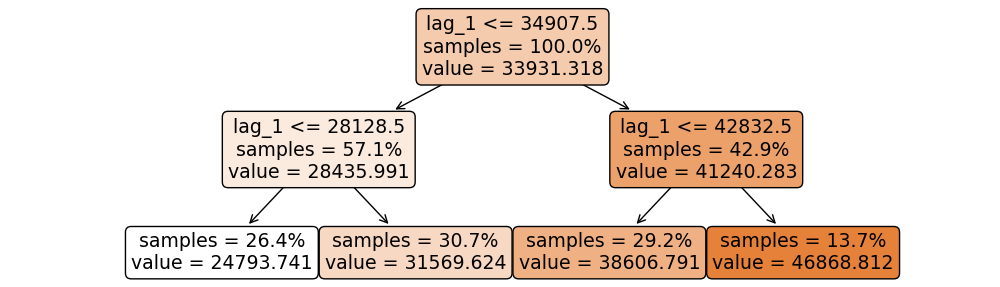
\includegraphics[width = 0.9\textwidth]{imagenes/reg_tree.png}
    \caption{Árbol de regresión}\label{fig:reg_tree}
\end{figure}

Este razonamiento se puede aplicar a las series temporales, a partir de un número de observaciones se puede pronosticar un nuevo valor de la serie. Como las series temporales describen una variable continua, se utilizará árboles de regresión. La Figura \ref{fig:reg_tree} representar un árbol de regresión que utilizan las diez últimas observaciones de la serie para predecir el siguiente valor, es decir, con los datos $\{X_{T-9}, \dotsc, X_{T-1}, X_T\}$ calcula la predicción $\hat{X}_{T+1}$.


Los CART son algoritmos muy eficaces, pero se puede mejorar su efectividad mediante nuevos métodos. En esta sección se estudia dos técnicas que combinan árboles de decisión para aumentar su fiabilidad, Random Forest y XGBoost.


Random Forest se basa en la combinación de múltiples CART individuales para realizar predicciones más precisas y estables. Cada árbol  se entrena de forma independiente en una muestra aleatoria del conjunto de datos de entrenamiento, utilizando diferentes subconjuntos aleatorios de características. Más tarde, cada árbol emite su propia predicción y, en el caso de clasificación, la predicción final se determina mediante la mayoría de votos de todos los árboles, mientras que en el caso de regresión, se calcula el promedio de las predicciones de todos los árboles. Este enfoque de combinación de múltiples modelos ayuda a reducir el sobreajuste y mejorar la precisión general del modelo. 


Por otra parte, XGBoost combina múltiples árboles de decisión de forma iterativa de forma que los árboles no son independientes. El modelo se inicia planteando un árbol de decisión simple, a continuación y de forma secuencial, los siguientes árboles se encargan de predecir los errores o residuos del árbol anterior, de esta forma se mejoran progresivamente las predicciones. Al finalizar, el modelo XGBoost utiliza la combinación ponderada de los árboles para generar una predicción final. La Figura \ref{fig:RF+XGB} muestra el funcionamiento de ambos algoritmos.


\begin{figure}[h]
\centering
    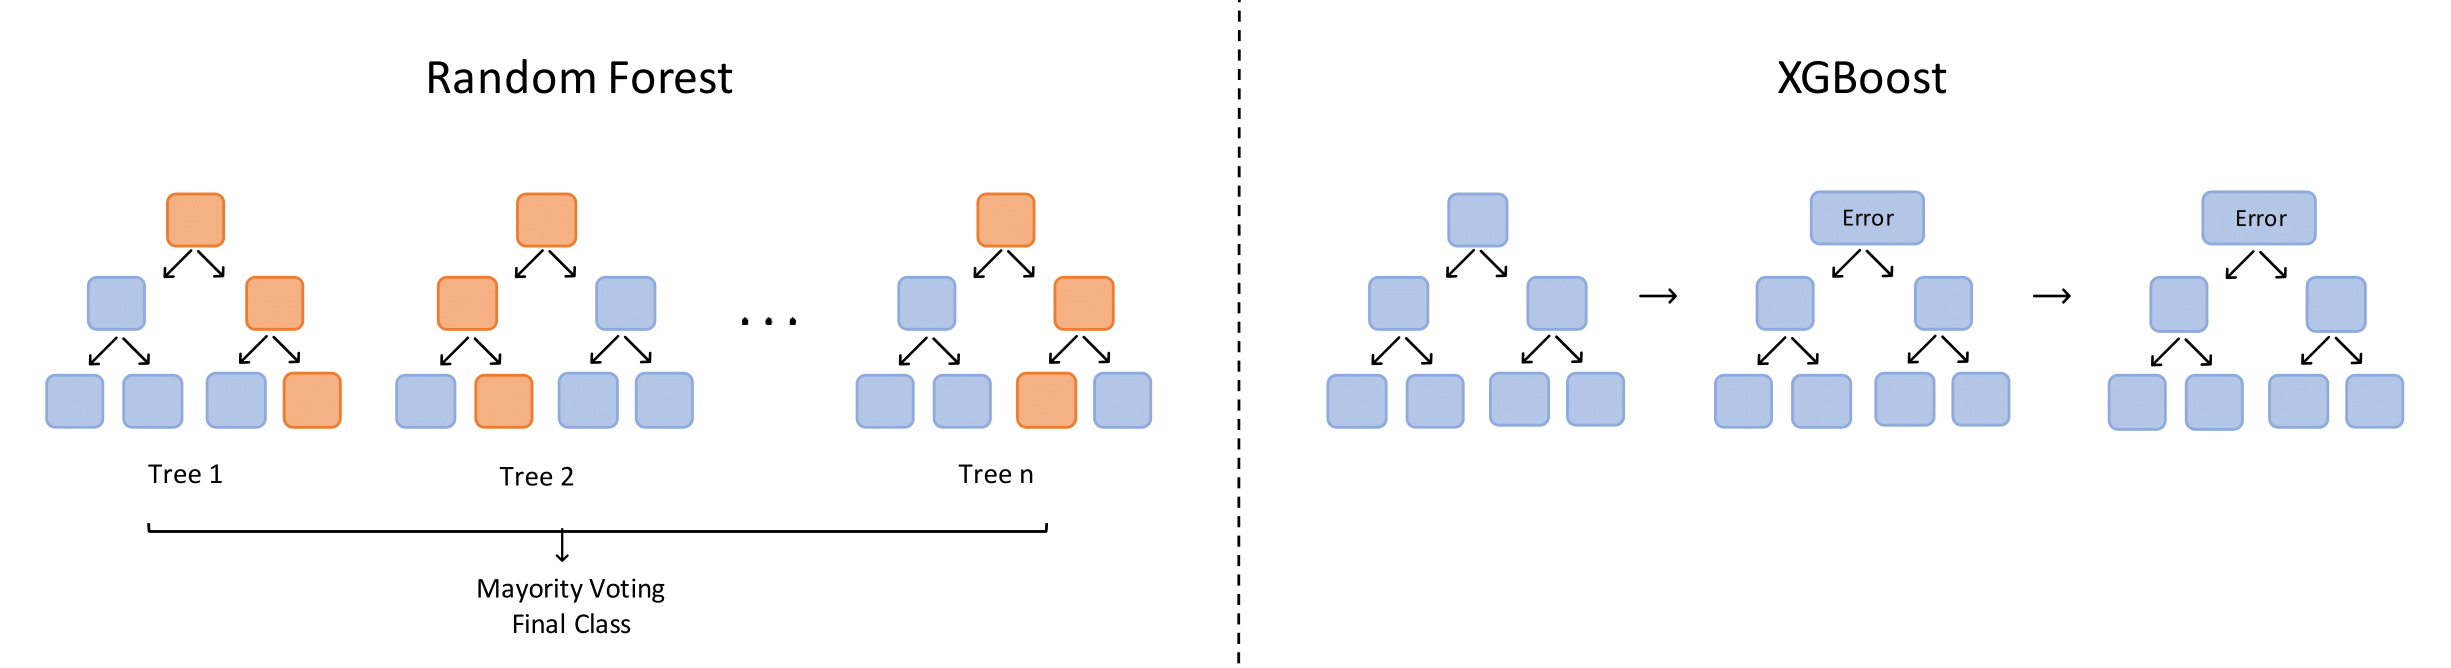
\includegraphics[width = \textwidth]{imagenes/RF+XGB.png}
    \caption{Funcionamiento de Random Forest y XGBoost}\label{fig:RF+XGB}
\end{figure}








Con los árboles de decisión se puede predecir el valor de una variable objetivo de estudio, sin embargo en el análisis de series temporales es interesante estudiar las predicciones en un intervalo futuro, para poder estudiar su evolución. Por esta razón surgen nuevos métodos que permiten generar este tipo de predicciones múltiples, los métodos multipaso o \emph{multi-step}. En Python, la implementación de estos métodos es a través del paquete \texttt{skforecast} \cite{DT2}.










\subsection{Método multipaso recursivo}
Supóngase que se dispone de datos de una serie temporal $\{X_1, \dotsc, X_T\}$ y se quiere predecir el valor de $X_{T+h}$. El funcionamiento de los árboles de decisión permite entrenar el modelo para predecir el siguiente valor de la serie, es decir, si se quiere predecir el valor $X_{T+h}$ se requiere conocer el valor de $X_{T+h-1}$, pero para conocer este valor es necesario tener el de $X_{T+h-2}$, y así. 

Este algoritmo es muy sencillo de implementar y consiste en utilizar los últimos $n$ valores de la serie temporal para predecir el próximo, $\hat{X}_{T+1}$. El siguiente paso utiliza los últimos $n-1$ valores de la serie y el nuevo valor pronosticado $\hat{X}_{T+1}$ para predecir el valor de $\hat{X}_{T+2}$. Así continua el algoritmo hasta obtener la predicción de $X_{T+h}$, se puede ver de forma esquemática en la Figura \ref{fig:multistep-recursive}.

\begin{figure}[h]
\centering
    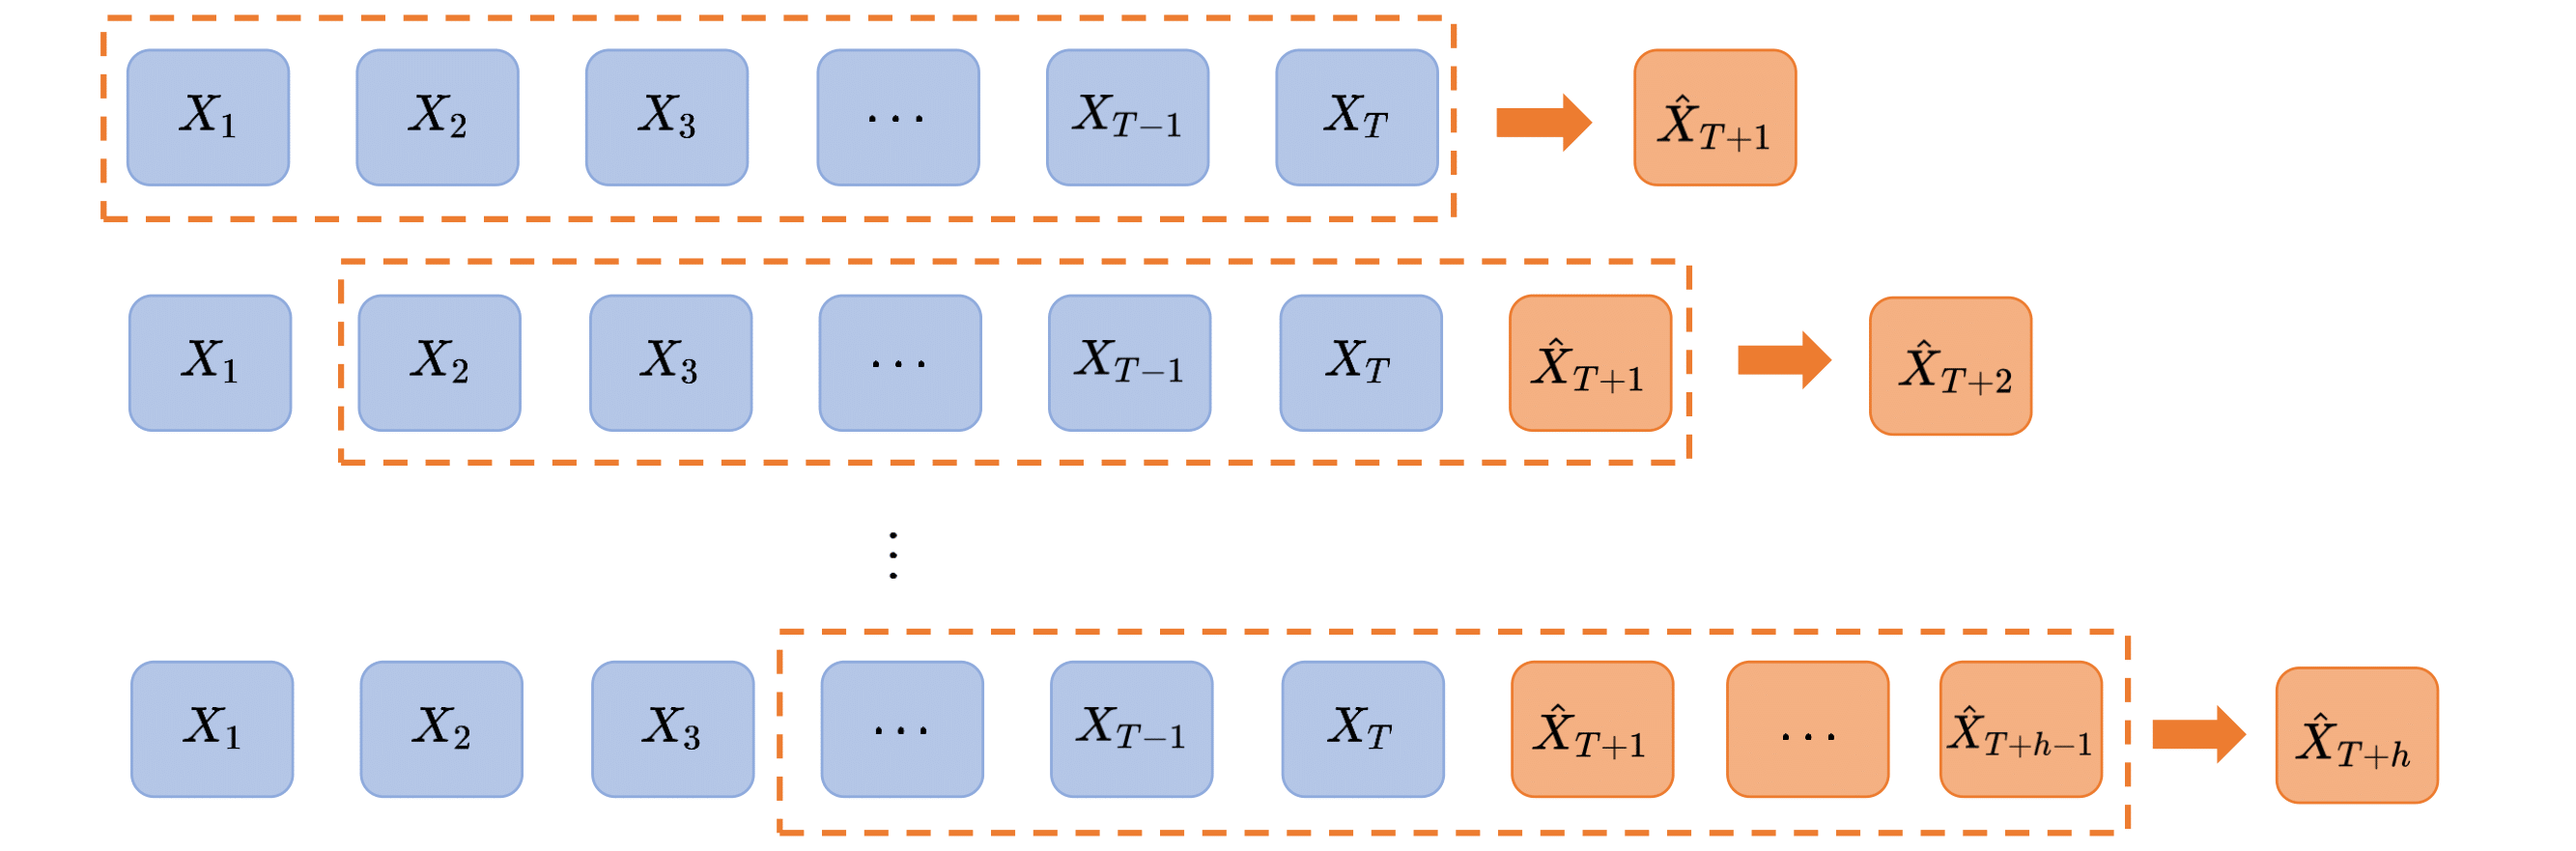
\includegraphics[width = 0.75\textwidth]{imagenes/multistep-recursive.png}
    \caption{Esquema del método multipaso recursivo con $n=T$}\label{fig:multistep-recursive}
\end{figure}


En la práctica, este algoritmo se ha aplicado con los métodos de Random Forest y XGBoost. La implementación de Python se realiza mediante la función \texttt{ForecasterAutoreg} y  permite elegir el número de retardos o lags, $n$, (parámetro \texttt{lags}) con los que se quiere trabajar, es decir, con cuántas observaciones se entrena el modelo. En este caso se ha probado dos valores $n=48$,  $n=48\cdot 7$ y $n=48\cdot 30$, los modelos se entrenan con los datos del día anterior, de la semana anterior y del mes anterior, respectivamente. 

Por otro lado, para indicar el regresor que se va utilizar se emplea el parámetro \texttt{regressor}, en este caso se utiliza las funciones \texttt{RandomForestRegressor} y \texttt{XGBRegressor}.


\begin{table}[h] 
\centering
\begin{tabular}{cccccc} \hline
& R\_RF1 & R\_RF2 & R\_XGB1 & R\_XGB2 & R\_XGB3 \\ \hline
MAPE   & $18.82$ &  $19.03$ & $13.128$ & $19.03$ & $14.97$  \\ 
MSE    & $5.02\cdot10^7$ &  $4.49\cdot10^7$ & $2.42\cdot10^7$ & $4.49\cdot10^7$ & $2.93\cdot10^7$ \\
Tiempo (s) & $96.238$  & $635.34$ & $17.30$ & $623.78$ & $2821.58$ \\ \hline
\end{tabular}
\caption{Comparación de los modelos del método multipaso recursivo} \label{tab:comp_autoreg}
\end{table}

En la Tabla \ref{tab:comp_autoreg} se ha llamado a los modelos por sus iniciales y el número corresponde a los lags con los que se ha trabajado, es decir, 1, 2 y 3 son un día, una semana y un mes, respectivamente. El tiempo de ejecución del modelo Random Forest trabajando con un mes de retardo es muy alto así que no se ha incluido. 

Se ve que, según aumenta la complejidad del modelo, también aumenta su tiempo de ejecución, como es lógico pensar. Por otra parte, el error MAPE alcanza valores entre $13\%$ y $20\%$, aunque no son menores a los valores del modelo Prophet. Todos los modelos presentan gráficas similares. En este caso, la Figura \ref{fig:XGBoost} muestra el modelo que utiliza XGBoost y los datos del mes anterior para predecir. 
\begin{figure}[h]
\centering
    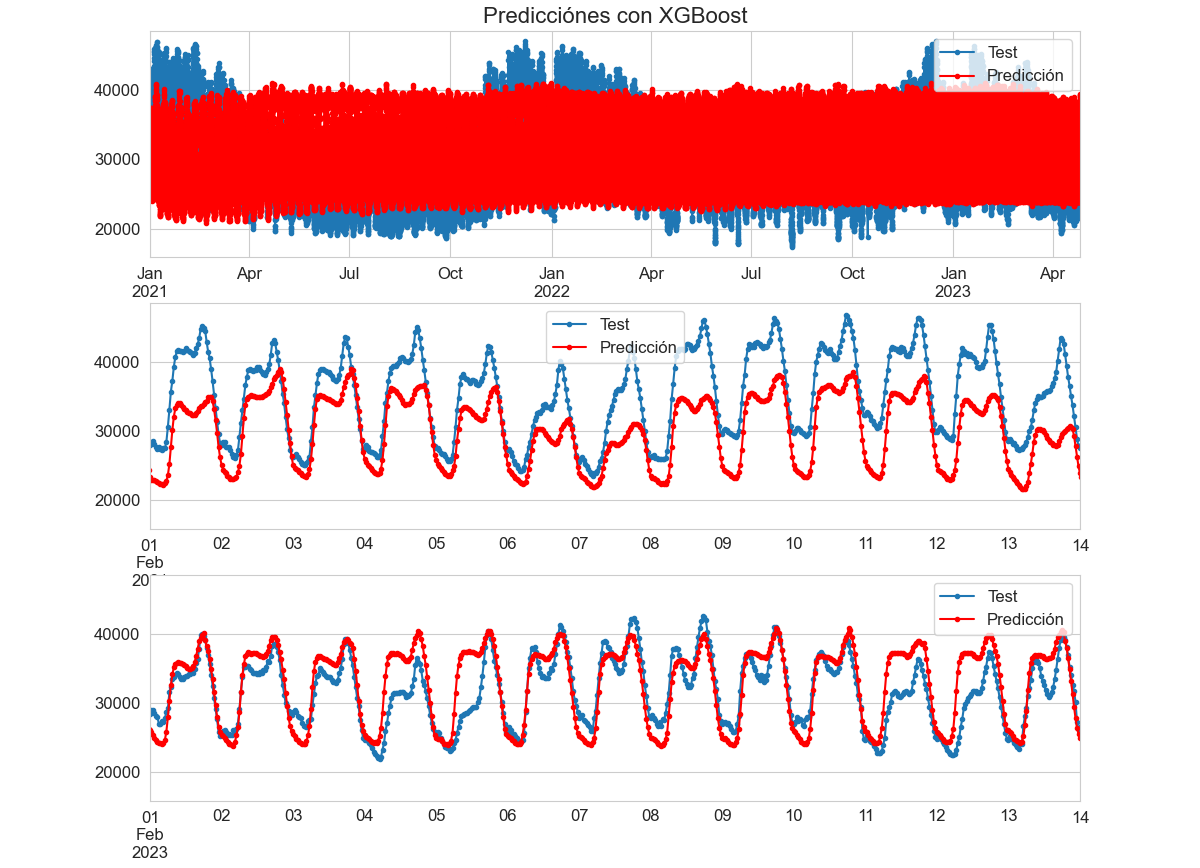
\includegraphics[width = 0.8\textwidth]{imagenes/XGBoost.png}
    \caption{Predicción con el modelo XGBoost (modelo R\_XGB3)}\label{fig:XGBoost}
\end{figure}


Se puede observar que el modelo no es capaz de predecir los patrones de estacionalidad que ocurren a lo largo de los años, aunque sí capta las fluctuaciones que ocurren durante las horas del día. El modelo a corto plazo predice correctamente las primeras observaciones del conjunto test. Sin embargo, a largo plazo las predicciones no son capaces de captar las diferencias entre los meses del año, puesto que las predicciones siempre se encuentran en el mismo nivel.

Sin duda estos algoritmos son muy útiles, pero es importante ajustar el número de retardos. En este caso el número de retardos que mejor ha funcionado se corresponde con la estacionalidad mensual. A la hora de aplicar el algoritmo es recomendable ajustar el número de lags de forma que alcance al menos un ciclo de estacionalidad, pero teniendo en cuenta que, para valores demasiados grandes, el algoritmo aumenta el tiempo de computación.




Todo esto motiva a buscar los parámetros que permitan ajustar correctamente los tipos de estacionalidad. Se va a trabajar con el modelo XGBoost por ser el algoritmo con mejor tiempo de ejecución. 

Adaptando los parámetros que ajustan la tasa de aprendizaje del modelo XGBoost, se consigue que se capte la estacionalidad anual, pero solamente en los primeros meses del test, como se ve en la Figura \ref{fig:XGBoost_adjust}. Los modelos presentados logran capturar la primera subida y la primera bajada del año 2022, pero conforme avanzan los años, las predicciones quedan estáticas.
\begin{figure}[h]
\centering
    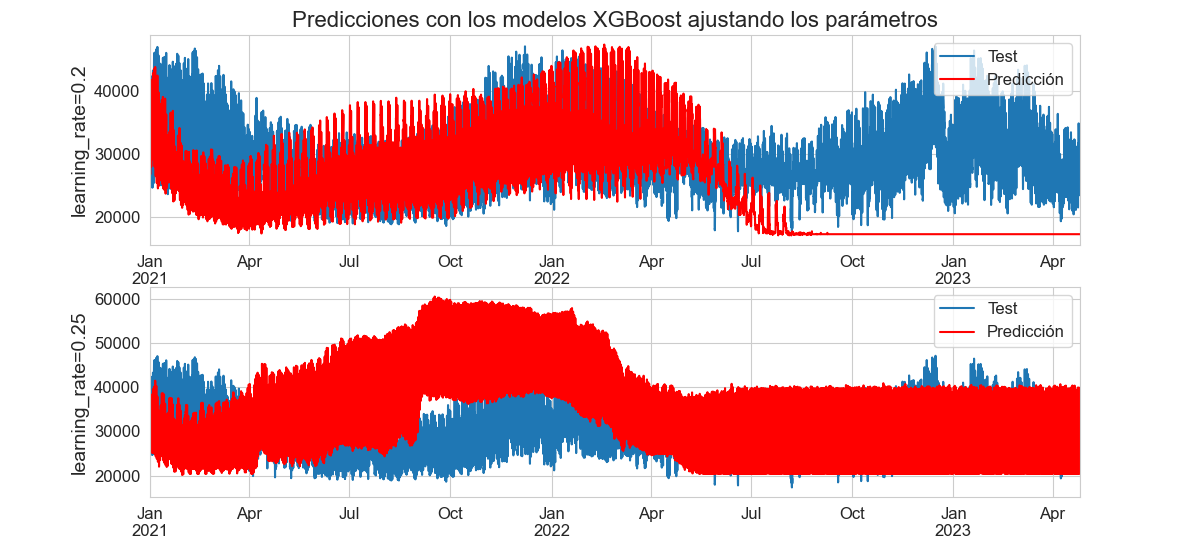
\includegraphics[width = 0.85\textwidth]{imagenes/XGBoost_adjust.png}
    \caption{Modelos XGBoost ajustados}\label{fig:XGBoost_adjust}
\end{figure}

En este caso, el error MAPE asciende hasta más del $25\%$, siendo el más alto de los modelos autorregresivos, pero también es el único en captar la estacionalidad anual. Por otra parte, los tiempos de ejecución son de alrededor de los $20$ minutos. 

% El cambio con los modelos anteriores es que ahora el primer retardo recoge una impotancia del $70\%$. Los lags $334$, $669$ y $3$ tienen una importancia del $1\%$ y, las demás variables son menores.

No se ha conseguido mejorar el error, sin embargo sí es posible pronosticar cambios anuales solamente entrenando con un mes de antelación. Disponiendo de un mayor número de lags que abarquen varios meses o un año completo, es más probable que el algoritmo recoja correctamente todos los cambios. Sin embargo, el tiempo de ejecución es una limitación y no se ha podido computar.



\subsection{Método multipaso directo}
El método multipaso recursivo no es el único capaz de predecir series temporales, en esta sección se estudia otro tipo de método multipaso: el método multipaso directo. Mientras el anterior algoritmo utiliza las predicciones que él mismo generaba, este método consiste en crear un modelo para cada predicción. En este caso, si se quiere predecir el valor de $X_{T+h}$, se crea un modelo que tome $n$ observaciones consecutivas de la serie temporal y prediga el valor para $h$ pasos hacia delante, como muestra la Figura \ref{fig:multistep-direct}.
\begin{figure}[h]
\centering
    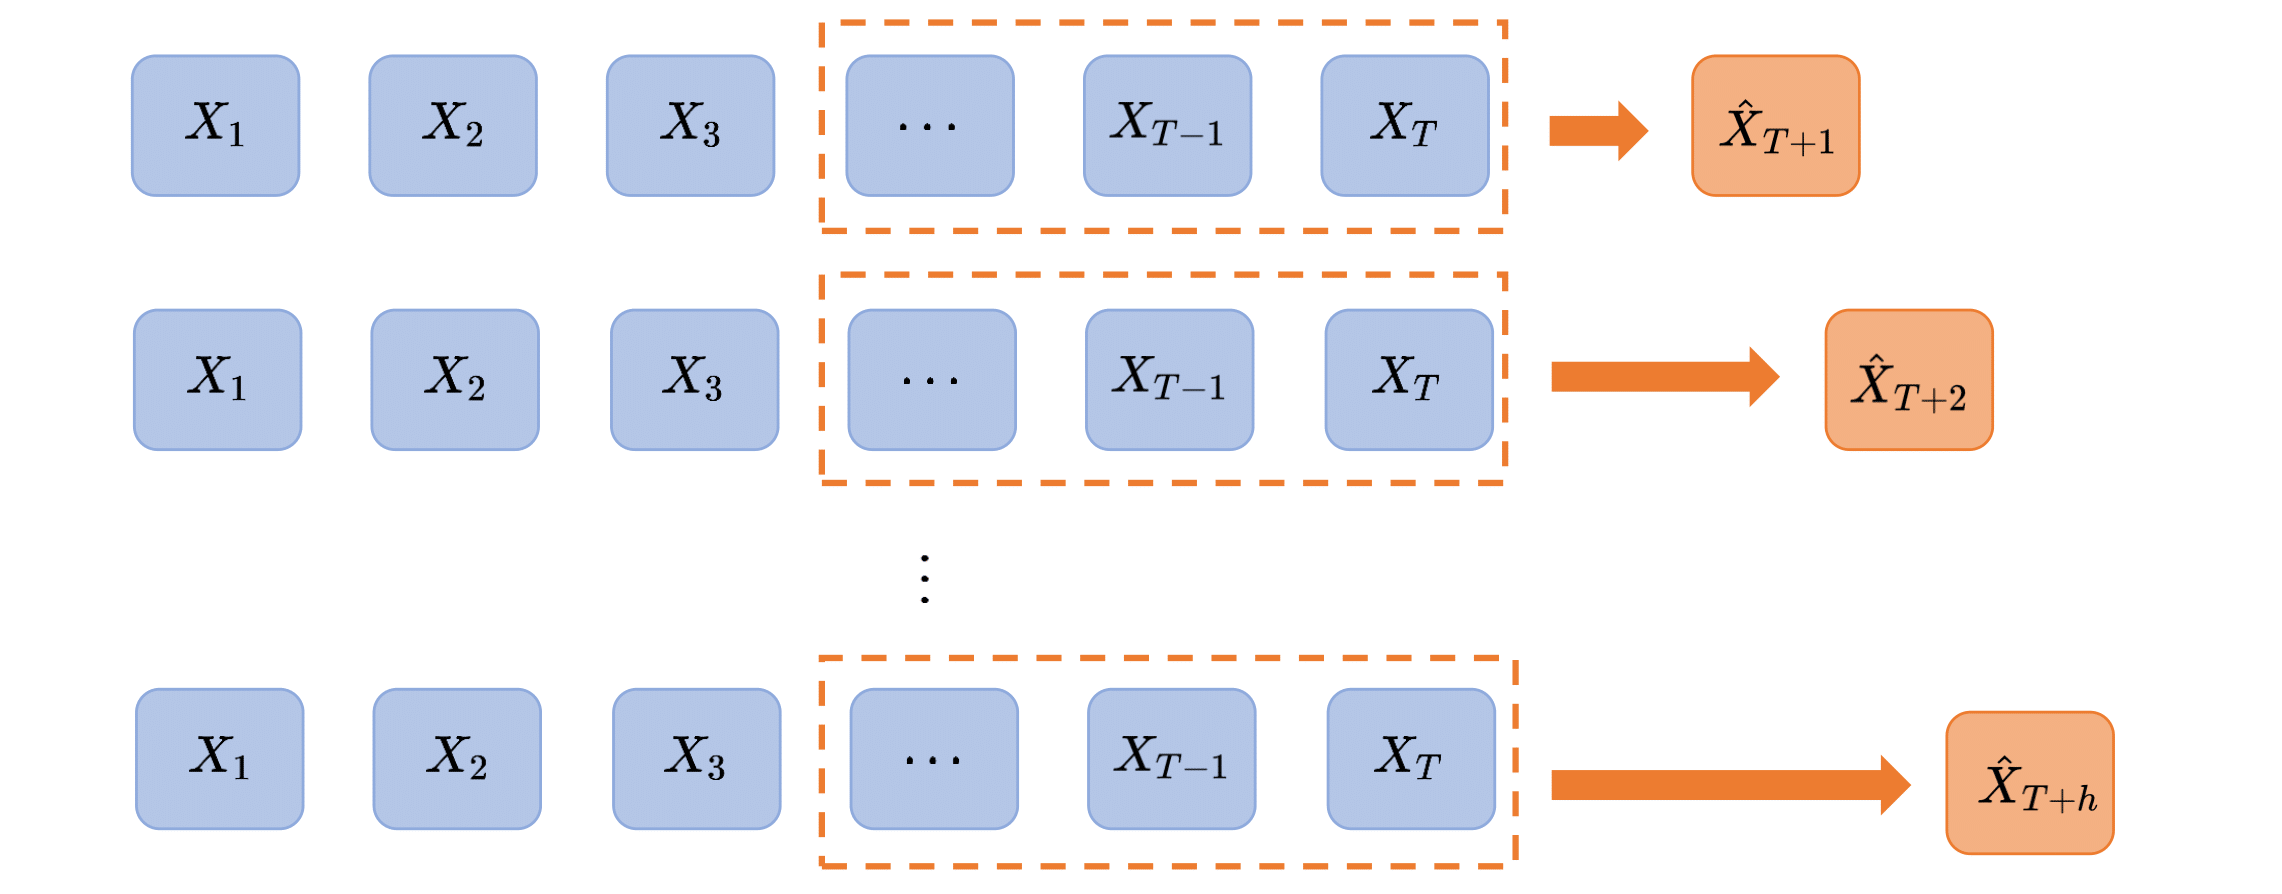
\includegraphics[width = 0.7\textwidth]{imagenes/multistep-direct.png}
    \caption{Esquema del método multipaso directo}\label{fig:multistep-direct}
\end{figure}


En el método anterior, se calculan todos los valores intermedios hasta $X_{T+h}$, mientras que en este modelo se obtiene directamente dicho valor. Si se quiere calcular todos los valores intermedios, entonces es necesario entrenar $h$ modelos distintos, lo que aumenta el coste computacional. Por consiguiente, si se intenta utilizar el dataset completo sería necesario ajustar $48$ modelos para predecir un solo día. Por esta razón, se ha decidido estudiar los resultados del algoritmo aplicado a los datos agregados de forma diaria. 

Al igual que en el método anterior, se va a ajustar los datos usando diferentes lags a través de la función \texttt{ForecasterAutoregDirect}. El número de pasos a predecir, $h$, se indica con el parámetro \texttt{steps}. Se emplean datos de la semana, mes y año anterior y los resultados se observan en la Tabla \ref{tab:comp_direct}.

\begin{table}[h]
    \centering
\begin{tabular}{ccccccc} \hline
& D\_RF1 & D\_RF2 & D\_RF3 & D\_XGB1 & D\_XGB2 & D\_XGB3 \\ \hline
MAPE   & $16.66$ &  $18.27$ & $7.34$ & $15.87$ & $17.14$ & $9.87$  \\ 
MSE    & $7.29\cdot10^{10}$ &  $9.44\cdot10^{10}$ & $1.73 \cdot10^{10}$ & $6.55\cdot10^{10}$ & $8.38\cdot10^{10}$ & $3.20\cdot10^{10}$ \\
Tiempo (s) & $139.67$  & $565.86$ & $8467.68$ & $26.97$ & $173.22$ & $1217.60$ \\ \hline
\end{tabular}
    \caption{Comparación de los modelos del método multipaso directo}
    \label{tab:comp_direct}
\end{table}

A continuación se muestran seis gráficas comparando la actuación de Random Forest y XGBoost para cada periodo de entrenamiento. En todos los casos se ha calculado las predicciones para los años 2021 y 2022.

\begin{figure}[h]
\centering
    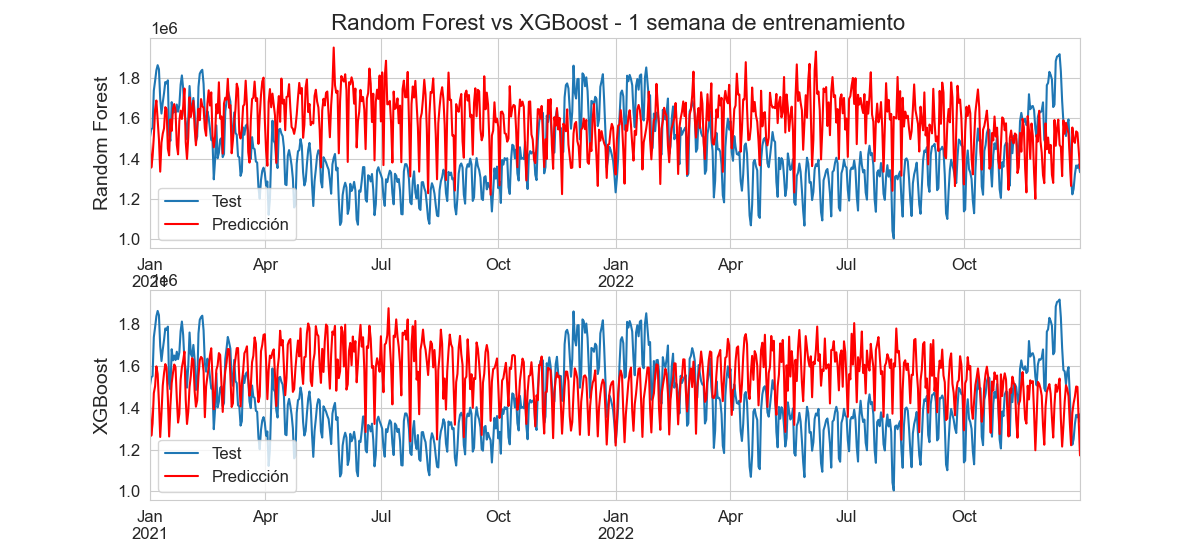
\includegraphics[width = 0.85\textwidth]{imagenes/autoreg_direct3.png}
    \caption{Modelos RandomForest y XGBoost con entrenamiento de una semana}\label{fig:autoreg_direct3}
\end{figure}

Las primeras dos gráficas, Figura \ref{fig:autoreg_direct3}, muestran las predicciones de los modelos RandomForest y XGBoost con entrenamiento de una semana. Ambos modelos tienen un comportamiento similar y resalta la forma en la que predice la estacionalidad anual. Muestra subidas en la serie para los meses de verano, donde realmente la demanda eléctrica desciende. El mínimo de la predicción se alcanza al inicio de cada año y en los datos también se produce esta bajada y subida, pero más abrupta. En ambos casos los errores MAPE son $16\%$ aproximadamente y el tiempo de ejecución cuatro veces mayor en el algoritmo RandomForest.

\begin{figure}[h]
\centering
    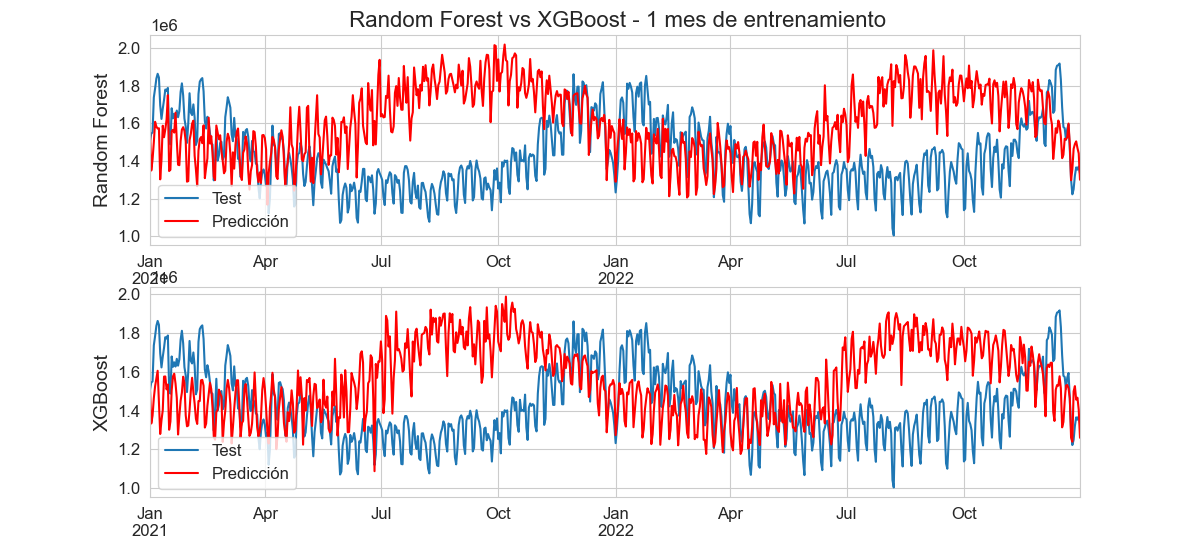
\includegraphics[width = 0.85\textwidth]{imagenes/autoreg_direct1.png}
    \caption{Modelos RandomForest y XGBoost con entrenamiento de un mes}\label{fig:autoreg_direct1}
\end{figure}

Las siguiente gráficas a estudiar se corresponden con los modelos entrenados con un mes de los datos, Figura \ref{fig:autoreg_direct1}. De nuevo, ambos gráficos tienen un comportamiento similar, se puede ver que ninguno es capaz de capturar el componente estacional que presentan los datos. Incluso parece que las predicciones están desplazadas, ya que predicen subidas y bajadas pero no se corresponden con los tiempos de la serie. En este caso los errores son mayores, con un valor de $18.27\%$ y $17.14\%$, respectivamente. Solo entrenando con un mes no es suficiente para ajustar correctamente los cambios estacionales, por ello, a continuación se ha estudiado los mismo modelos pero con entrenamiento de un año completo.


\begin{figure}[h]
\centering
    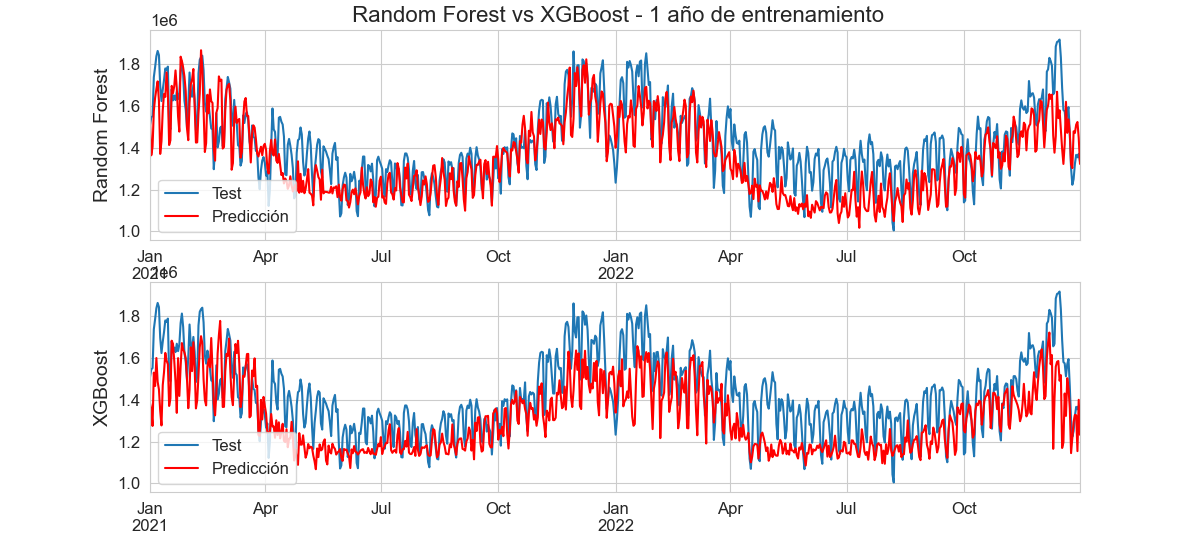
\includegraphics[width = 0.85\textwidth]{imagenes/autoreg_direct2.png}
    \caption{Modelos RandomForest y XGBoost con entrenamiento de un año}\label{fig:autoreg_direct2}
\end{figure}

Las siguientes gráficas se corresponden al entrenamiento de un año, se pueden ver en la Figura \ref{fig:autoreg_direct2}. Hay mejora notable a la hora de predecir la estacionalidad, en este caso los errores MAPE son $7.34\%$ y $9.87\%$, respectivamente, por tanto, el método de Random Forest minimiza el error en este caso.


Cabe resaltar la importancia de los retardos con los que se entrena el modelo. En este caso ha marcado un cambio importante, siendo capaz de ajustar la estacionalidad del modelo. Un inconveniente de este tipo de algoritmos es su tiempo de ejecución, pues es necesario entrenar un modelo por cada predicción que se quiere hacer, lo que provoca que sea complicado producir predicciones a largo plazo. Sin embargo, con los datos trabajados, se obtiene una buena predicción con un error MAPE de $7.34\%$, el menor hasta ahora. También cabe señalar que el tiempo de ejecución del modelo RandomForest es $7$ veces mayor al XGBoost en este caso.



La implementación en Python a través de la funciones \texttt{ForecasterAutoreg} y  \texttt{Forecas- terAutoregDirect} permite además añadir variables exógenas al modelo a través del parámetro \texttt{exog} y su funcionamiento es distinto según si el método es recursivo o directo. 

Para el método multipaso recursivo se utiliza las predicciones de la variable exógena para computar las predicciones de la variable objeto de estudio como se ha explicado en la Sección \ref{sec:SARIMA}. 

Por otro lado, para el método multipaso directo se crea un modelo para cada predicción que se realiza, por tanto, si se incluye una variable exógena también se utiliza los valores de la variable exógena del conjunto entrenamiento. En este caso, no es necesario utilizar valores futuros de la variable exógena.

A través de la variables exógenas es posible añadir nueva información a la serie temporal. De esta forma, se puede introducir una variable binaria que indique si un día es festivo para modelar los efectos vacacionales. 

Se ha comprobado que, ajustando el número de retardos, es posible modelar el componente estacional de la serie. No obstante, no se ha mencionado el componente de tendencia. Si los datos de la serie temporal presentan un crecimiento o decrecimiento y, además, se dividen en los conjuntos train y test, de forma que el rango de la serie en el test no está incluido en el rango de train, surge un problema. Los árboles de regresión devuelven la media de los valores de la hoja correspondiente, con lo cual estos valores estarán incluidos en el rango del train y no del test. Por tanto, las predicciones no pueden extrapolar la tendencia de la serie.

Se puede solventar este problema añadiendo variables exógenas que describan los cambios de tendencia, como puede ser los ratios o los promedios móviles de la serie. De esta forma, sí es posible modelar la tendencia con modelos autorregresivos basados en árboles de regresión.


Una ventaja de utilizar el paquete \texttt{skforecast} es que hay implementadas otras funciones para evaluar los modelos, como por ejemplo la función \texttt{backtesting\_forecaster}. El \emph{bakctesting} es el proceso de evaluar el rendimiento de un modelo utilizando datos históricos.

Durante el backtesting, se ajusta el modelo a los datos de entrenamiento y se generan pronósticos para los periodos de prueba. Luego, se comparan los pronósticos con los valores reales conocidos para evaluar qué tan precisos son. Esto ayuda a determinar la capacidad del modelo para capturar patrones y tendencias en los datos históricos y pronosticar de manera efectiva los valores futuros.








\newpage
\section{Comparación de modelos}
En este trabajo se han estudiado cuatro modelos de predicción para series temporales, dos de ellos clásicos y dos de reciente creación.

En cuanto a los modelos clásicos, procesos SARIMA y método de suavizado exponencial, cabe destacar su limitación a la hora de trabajar con los datos. La gran dimensión de las variables y el tamaño del periodo de estacionalidad ($s=48\cdot 365$) ha provocado que el tiempo de computación sea tan alto, hasta llegar a ser impracticable.

Sin embargo, aplicados a los datos agregados sí funcionan correctamente y son capaces de modelizar la estacionalidad. Para casos con menor envergadura de datos y tamaño de estacionalidad inferior, los métodos funcionan correctamente.

En cuanto a los modelos más recientes, el método multipaso directo no ha podido modelar los datos debido, también, a su tiempo de ejecución, ya que es necesario un modelo para cada predicción. Por tanto, solamente el algoritmo Prophet y el método multipaso recursivo han sido capaces de crear modelos consistentes con la tendencia y estacionalidad de los datos.

Una diferencia clara entre los métodos clásicos y los no clásicos es que los métodos clásicos vistos no son capaces de trabajar con varios tipos de estacionalidad. Se ha visto que el algoritmo de Prophet puede modular la estacionalidad diaria, semanal, mensual y anual a la vez, lo que hace de este método una herramienta muy potente y eficaz. Además, incorpora un componente único, el componente vacacional.

\begin{table}[h] 
\centering
\begin{tabular}{cccccc} \hhline{~~----} 
& & Tendencia & Estacionalidad & Vacaciones & \begin{tabular}[c]{@{}l@{}}Variables\\ exógenas\end{tabular} \\ \hline 
SARIMA & & \cmark & \cmark & \xmark & \cmark \\ \hline 
\multirow{ 3}{*}{\begin{tabular}[c]{@{}c@{}}Exponential\\ Smoothing\end{tabular}} & Simple& \xmark & \xmark & \xmark & \xmark\\ 
& Doble & \cmark & \xmark & \xmark & \xmark \\ 
& Triple & \cmark & \cmark & \xmark & \xmark\\ \hline 
Prophet & & \cmark & \cmark & \cmark & \cmark\\ \hline
\begin{tabular}[c]{@{}c@{}}Modelos\\ autorregresivos\end{tabular} & & \cmark & \cmark & \cmark & \cmark\\ \hline

\end{tabular}
\caption{Componentes de los modelos} \label{tab:comp_mod}
\end{table}



La Tabla \ref{tab:comp_mod} muestra los componentes que poseen y carecen los modelos estudiados. Los modelos que siguen métodos autorregresivos no parten de una descomposición de series temporales, por lo que es más complicado medir su capacidad. El ajuste de estos modelos depende de los parámetros del modelo escogido y de los retardos usados. Cuanto mayor sea el número de lags, el modelo tendrá más datos para aprender sobre la tendencia y estacionalidad de la serie, sin embargo el tiempo de ejecución aumenta. Se ha visto que es posible modelar los diferentes componentes a través de los datos de la serie o añadiendo otras variables exógenas que indican otros cambios de los datos. En resumen, tres de los cuatro modelos pueden incorporar variables exógenas a la serie.



En este trabajo se ha estudiado los modelos aplicados a los datos agregados de forma diaria y a los datos completos. A continuación, se estudia y compara el error MAPE y tiempo de ejecución de los modelos.
\begin{figure}[h]
\centering
    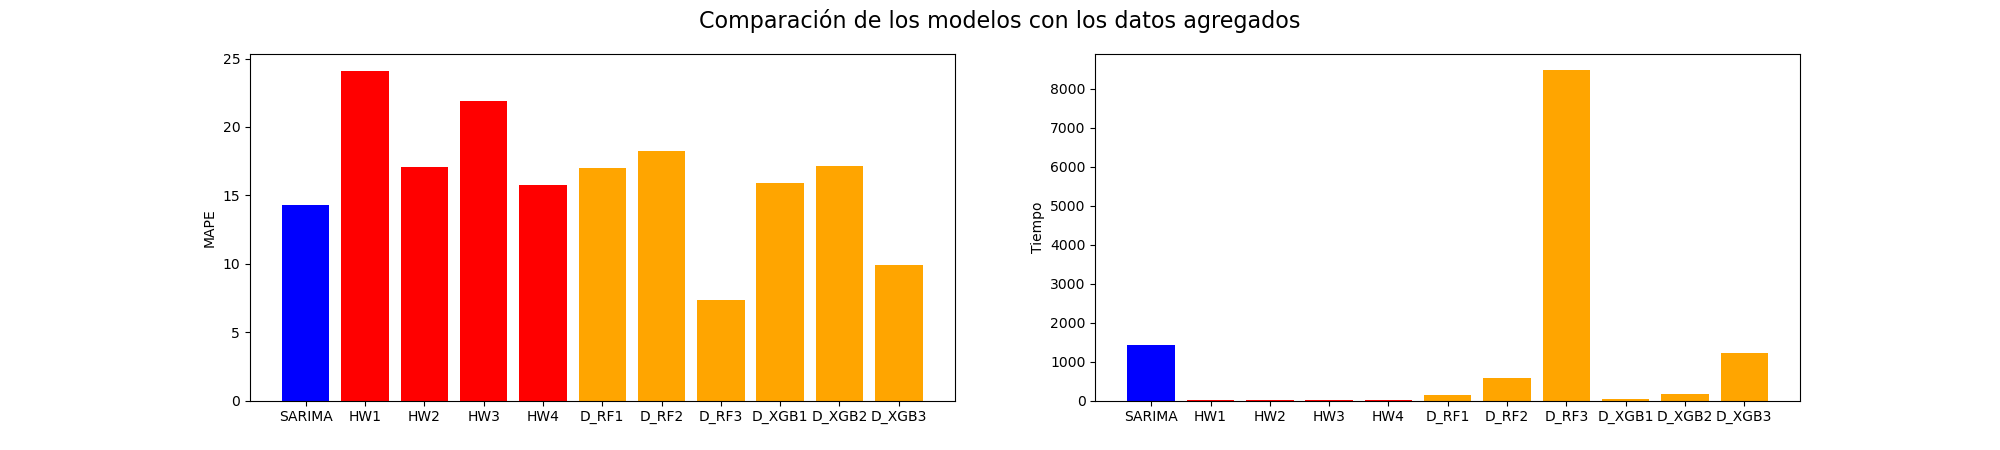
\includegraphics[width = \textwidth]{imagenes/comp_final2.png}
    \caption{Comparación según el MAPE y el tiempo de los modelos SARIMA, Holt-Winters y los métodos autorregresivos multipaso directo}\label{fig:comp_final2}
\end{figure}

La Figura \ref{fig:comp_final2} muestra el error y tiempo de ejecución de los modelos SARIMA, Holt-Winters y los métodos autorregresivos de multipaso directo. En este caso, el modelo que minimiza el error MAPE es el modelo autorregresivo que utiliza RandomForest y un año de entrenamiento, con un valor del $7.29\%$. Éste es uno de los modelos con mayor tiempo de ejecución, con un tiempo de más de $2$ horas.
\begin{figure}[h]
\centering
    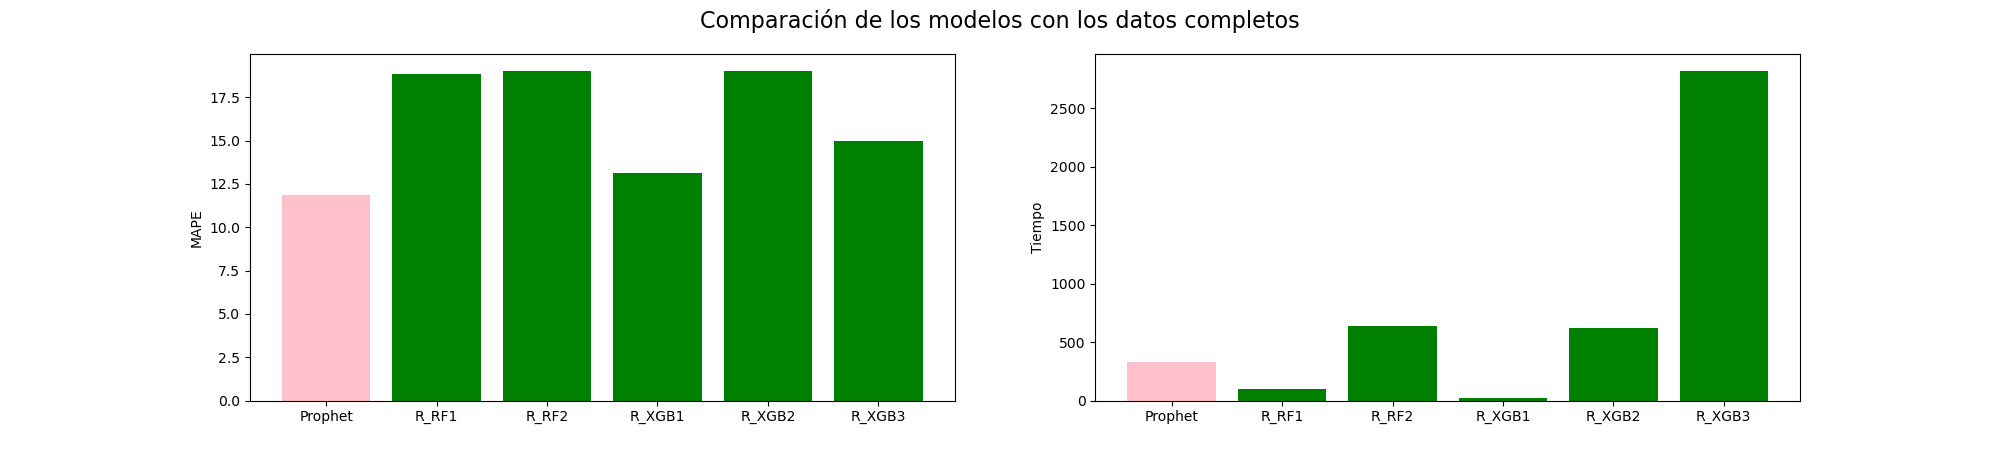
\includegraphics[width = \textwidth]{imagenes/comp_final1.png}
    \caption{Comparación según el MAPE y el tiempo del modelo Prophet y los métodos autorregresivos multipaso recursivo}\label{fig:comp_final1}
\end{figure}


Por otra parte, la Figura \ref{fig:comp_final1} muestra el error y tiempo de computación de los modelos que han ajustado los datos completos. En este caso, el error lo minimiza el algoritmo de Prophet, con un valor del $11.83\%$. Éste es el algoritmo que mejor ha funcionado con los datos disponibles en todo momento, además presenta una forma sencilla de ajustar los parámetros.

Encontrar un término medio entre una buena predicción y un buen tiempo de ejecución ha sido un punto clave en este trabajo. No cabe duda de que el modelo que ha cumplido con las expectativas es el modelo Prophet.

Los modelos autorregresivos presentan un error similar al de Prophet, sin embargo, no han conseguido modelar todos los tipos de estacionalidad. Añadiendo variables exógenas o aumentando el número de lags es posible cumplir este cometido. No obstante, también requiere una gran inversión de tiempo de programación y ejecución del que no se dispone, ya que se estudian muchos otros métodos en el proyecto.


La Tabla \ref{Comp_modelos} es una comparación de todos los modelos usados donde se ha añadido su implementación en Python y algunas consideraciones a tener en cuenta a la hora de usarlos.

\newpage

\begin{landscape}
\begin{table}
\centering
\resizebox{\columnwidth}{!}{%
\begin{tabular}{|ll|l|l|l|l|l|}
\hline
\rowcolor[HTML]{C0C0C0} 
\multicolumn{2}{|l|}{\cellcolor[HTML]{C0C0C0}Algoritmo} &
  Implementación Python &
  Parámetros principales &
  Control del overfitting &
  \begin{tabular}[c]{@{}l@{}}Coste \\ computacional\end{tabular} &
  Observaciones \\ \hline
\multicolumn{2}{|l|}{\cellcolor[HTML]{EFEFEF}SARIMA} &
  \begin{tabular}[c]{@{}l@{}}\texttt{statsmodels}\\ - \texttt{ARIMA}\\ - \texttt{SARIMAX}\end{tabular} &
  \begin{tabular}[c]{@{}l@{}}- \texttt{order(p,d,q)}.\\ - \texttt{seasonal\_order(P,D,Q,s)}.\\ - \texttt{trend}: determina el orden de la tendencia\\ ('c': constante, 't': lineal,  lista : grado del polinomio). \\ - \texttt{exog}: variables exógenas.\end{tabular} &
  \begin{tabular}[c]{@{}l@{}}- Reducir el valor de los órdenes.\\ - Reducir el grado de la tendencia. \end{tabular} &
  Medio &
  \begin{tabular}[c]{@{}l@{}}- Identificación mediante la metodología de \\ Box-Jenkins.\\ - Existen otros métodos que encuentran \\ el orden automáticamente (\texttt{auto.arima}).\\ - Se puede añadir variables exógenas.\end{tabular} \\ \hline
\multicolumn{1}{|l|}{\cellcolor[HTML]{EFEFEF}} &
  \cellcolor[HTML]{EFEFEF}Simple &
   &
  - \texttt{smoothing\_level}: $\alpha$. &
   &
   &
  \begin{tabular}[c]{@{}l@{}}- Solo modela datos que no presentan tendencia \\ ni estacionalidad.\end{tabular} \\ \cline{2-2} \cline{4-4} \cline{7-7} 
\multicolumn{1}{|l|}{\cellcolor[HTML]{EFEFEF}} &
  \cellcolor[HTML]{EFEFEF}\begin{tabular}[c]{@{}l@{}}Doble\\ (Holt)\end{tabular} &
   &
  \begin{tabular}[c]{@{}l@{}}- \texttt{smoothing\_level}: $\alpha$.\\ - \texttt{smoothing\_trend}: $\beta^*$.\\ - \texttt{damped\_trend = True/False}.\end{tabular} &
   &
   &
  - Solo modela datos que no presentan tendencia. \\ \cline{2-2} \cline{4-4} \cline{7-7} 
\multicolumn{1}{|l|}{\multirow{-6.5}{*}{\cellcolor[HTML]{EFEFEF}\begin{tabular}[c]{@{}l@{}}Exponential \\ Smoothing\end{tabular}}} &
  \cellcolor[HTML]{EFEFEF}\begin{tabular}[c]{@{}l@{}}Triple\\ (Holt-Winters)\end{tabular} &
  \multirow{-6.5}{*}{\begin{tabular}[c]{@{}l@{}}\texttt{statsmodels}\\ - \texttt{SimpleSmoothing}\\ - \texttt{Holt}\\ - \texttt{ExponentialSmoothing}\end{tabular}} &
  \begin{tabular}[c]{@{}l@{}}- \texttt{smoothing\_level}: $\alpha$.\\ - \texttt{smoothing\_trend}: $\beta^*$.\\ - \texttt{smoothing\_seasonal}: $\gamma$.\\ - \texttt{damped\_trend = True/False}.\end{tabular} &
  \multirow{-6.5}{*}{\begin{tabular}[c]{@{}l@{}}- Ajustar los parámetros de suavizado \\ cercanos a cero reduce los efectos de \\ los componentes de nivel, tendencia o \\ estacionalidad.\end{tabular}} &
  \multirow{-6.5}{*}{Medio-Bajo} &
  \begin{tabular}[c]{@{}l@{}}- Es capaz de modelar datos con tendencia y \\ estacionalidad.\\ - El aumento en el número de observaciones \\ provoca un aumento considerable en el \\ tiempo de ejecución.\end{tabular} \\ \hline
\multicolumn{2}{|l|}{\cellcolor[HTML]{EFEFEF}Prophet} &
  \begin{tabular}[c]{@{}l@{}}\texttt{fbprophet}\\ - \texttt{Prophet}\end{tabular} &
  \begin{tabular}[c]{@{}l@{}}- \texttt{n\_changepoints}: número de puntos de cambio de tendencia.\\- \texttt{changepoint\_range}: $\%$ del conjunto train al que aplicar \\ los puntos de cambio.\\- \texttt{holidays}: dataframe con los días festivos.\\ - \texttt{changepoint\_prior\_scale}:  $\tau$.\\ - \texttt{seasonality\_prior\_scale}: $\sigma^2$.\\ - \texttt{holiday\_prior\_scale}:  $\nu^2$. \end{tabular} &
  \begin{tabular}[c]{@{}l@{}}- Reducir el número de puntos de \\ cambio mediante \texttt{changepoint\_prior\_scale}.\\ - Reducir los efectos de la estacionalidad.\end{tabular} &
  Medio &
  \begin{tabular}[c]{@{}l@{}}- Modela un número ilimitado de tipos\\ de estacionalidad.\\ - Añade efecto de las vacaciones. \\ - Se puede añadir variables exógenas \\ mediante \texttt{add\_regressor}.\end{tabular} \\ \hline
\multicolumn{2}{|l|}{\cellcolor[HTML]{EFEFEF}Autorregresores} &
  \begin{tabular}[c]{@{}l@{}}\texttt{skforecast}\\ - \texttt{ForecasterAutoreg}\\ - \texttt{ForecasterAutoregDirect}\end{tabular} &
  \begin{tabular}[c]{@{}l@{}}- \texttt{regressor}: nombre del regresor, en este caso \\ \texttt{RandomForestRegressor} o \texttt{XGBRegressor}.\\ - \texttt{lags}: número de retardos ($n$).\\ - \texttt{steps}: pasos a predecir ($h$). \\ - \texttt{exog}: variables exógenas.\end{tabular} &
  \begin{tabular}[c]{@{}l@{}}- Reducir el número de lags con los que\\  se entrena.\\ - Parámetros intrínsecos de los árboles, \\ como reducir el número de estimadores \\ o añadir criterios de parada.\end{tabular} &
  Medio-Alto &
  \begin{tabular}[c]{@{}l@{}}- Se puede utilizar otros regresores que no sean \\ árboles de decisión.\\ - Utilizar un valor de \texttt{lags} similar a la \\ estacionalidad que se desea modelar. \\ - Se puede añadir variables exógenas. \end{tabular} \\ \hline
\end{tabular}%
}
\caption{Resumen de los modelos}
\label{Comp_modelos}
\end{table}
\end{landscape}







\newpage
\section{Conclusiones}
A lo largo de este trabajo se ha estudiado diferentes tipos de modelos. Se ha explicado en detalle el desarrollo matemático de los algoritmos, de la mano de su implementación en Python.


Ha sido una gran labor de investigación del funcionamiento de los algoritmos así como de aprender a implementarlos en Python. Los modelos SARIMA y de alisado exponencial ofrecen buenas predicciones, pero funcionan mejor con datos de menor dimensión.

Se ha visto que los modelos más eficaces son los más recientes, destacando la actuación del modelo Prophet. El algoritmo de Prophet es capaz de modelar distintos tipos de tendencia (lineal o logística) y un número ilimitado de componentes estacionales. Además, incluye una componente vacacional y la posibilidad de añadir otras variables exógenas a la serie. Su tiempo de computación es medio, es decir, para datos de menor tamaño puede ofrecer predicciones al instante y, para datos de mayor envergadura, como los tratados en este trabajo funciona correctamente con un tiempo de ejecución aproximado de $20$ minutos. 

Otra de las ventajas del algoritmo de Prophet es su sencilla implementación en Python que permite ajustar el modelo a partir de unos parámetros intuitivos. De igual manera existen muchas otras funciones en el paquete \texttt{fbprophet} que no se han mencionado, que permiten visualizar y trabajar con los datos de forma simple.

El objetivo del análisis de series temporales es la predicción de valores futuros de la serie, por ello se ha tomado el modelo de Prophet, ajustándolo a todos los datos disponibles para predecir el valor de la demanda eléctrica durante todo el año 2023.

\begin{figure}[h]
\centering
    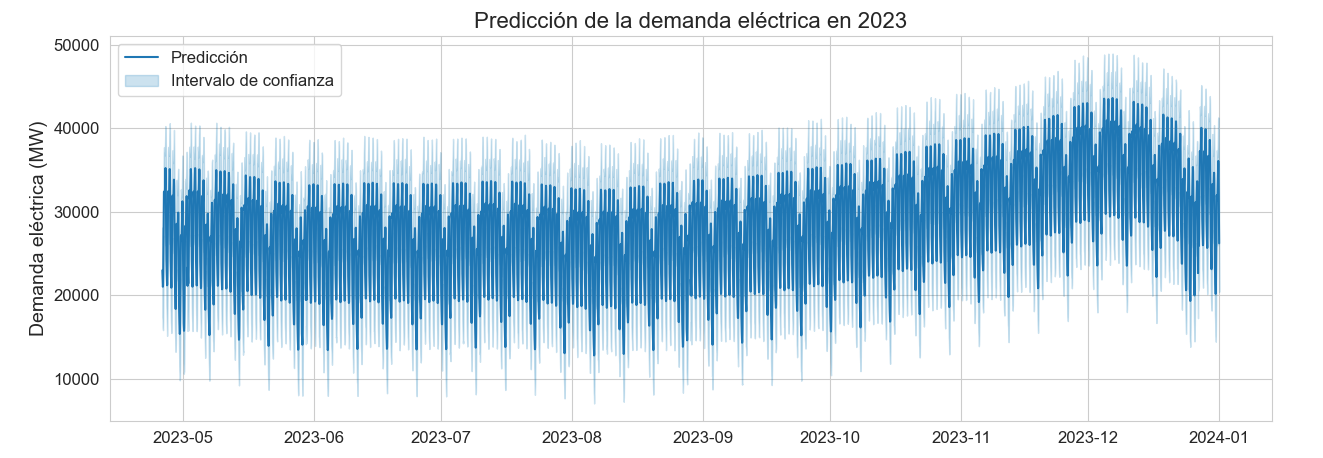
\includegraphics[width = \textwidth]{imagenes/prophet_future_predition.png}
    \caption{Predicción de la demanda eléctrica en Reino Unido durante 2023}\label{fig:prophet_future}
\end{figure}

La predicción se muestra en la Figura \ref{fig:prophet_future}. Se espera una subida de la demanda eléctrica durante el último trimestre de 2023 y una bajada brusca en las tres últimas semanas del año. Los valores de la demanda fluctúan entre los valores $20000$ y $35000$ MW a lo largo del año, hasta la subida que asciende hasta los $40000$ MW.



El mayor beneficio de realizar este trabajo ha sido aprender a modelar un caso real de series temporales, viendo las limitaciones y las ventajas de cada método. Así también, profundizando  las bases matemáticas que fundamentan los modelos para poder llevarlos a la práctica con rigor y buen criterio.

En este trabajo se ha profundizado en dos métodos de creación reciente, pero existen otros que no se han podido tratar. Las redes neuronales ofrecen resultados rápidos y eficientes. Este proyecto se puede extender profundizando en la redes neuronales recurrentes, en particular en la LSTM (\emph{Long-Short Term Memory}), ya que su planteamiento dista de todo lo estudiado hasta ahora. Todo esto puede dar paso a la ampliación de este trabajo o al planteamiento de un nuevo proyecto de investigación centrado en otros métodos de predicción como las redes neuronales.









%-------------------------------------------------------------------------------------------------------

\newpage
\addcontentsline{toc}{section}{Referencias}
\begin{thebibliography}{100}

\bibitem{TS1} Brockwell, P.J., Davis, R.A.  (1987).
\textit{Time Series: Theory and Methods}. Springer.


% \bibitem{TS3} Brockwell, P.J., Davis, R.A.  (1996).
% \textit{Introduction to Time Series and Forecasting}. Springer.

\bibitem{TS4} Box, G. E. P., Jenkins, G. M, Reinsel, G.C, Ljung, G.M.  (1970).
\textit{Time series analysis: Forecasting and control}. Wiley.

\bibitem{TS5} Perktold, J., Seabold, S., Taylor, J. Autoregressive Moving-Average Processes (ARMA) and Kalman Filter. \href{https://www.statsmodels.org/stable/ tsa.html\#autoregressive-moving-average-processes-arma-and-kalman-filter}{https://www.statsmodels.org/stable/ tsa.html\#autoregressive-moving-average-processes-arma-and-kalman-filter} (Consultado el 1 de julio de 2023).



\bibitem{ES1} Brown, R. G. (1963). \textit{Smoothing, forecasting and prediction of
discrete time series}. Dover Phoenix Editions.

\bibitem{ES2} Holt, C.C. (2004). \textit{Forecasting seasonals and trends by exponentially weighted moving averages. International Journal of Forecasting} \textbf{20}, 5-10.

\bibitem{ES3} Winters, P.R. (1960) \textit{Forecasting sales by exponentially weighted
moving averages. Management Science} \textbf{6}, 324 – 342 

\bibitem{ES4} Perktold, J., Seabold, S., Taylor, J. Exponential Smoothing. \href{https://www.statsmodels.org/stable/tsa.html\#exponential-smoothing}{https://www. statsmodels.org/stable/tsa.html\#exponential-smoothing} (Consultado el 1 de julio de 2023).


\bibitem{Prophet1} Taylor S.J., Letham B. (2017). \textit{Forecasting at scale}.

\bibitem{Prophet2} Taylor S.J., Letham B., Propeht Documentation. \href{https://facebook.github.io/prophet/docs/installation.html}{https://facebook.github.io/ prophet/docs/installation.html} (Consultado el 1 de julio de 2023).





\bibitem{DT1} Breiman, L., Friedman, J.H, Olshen, R.A. and Stone, C.J. (1984). Classification
And Regression Trees. Routledge

\bibitem{DT2} Amat, R., Escobar, J., Skforecast: forecasting series temporales con Python y Scikit-learn. \href{https://www.cienciadedatos.net/documentos/py27-forecasting-series-temporales-python-scikitlearn}{https://www.cienciadedatos.net/documentos/py27-forecasting-series-temporales-python-scikitlearn} (Consultado el 1 de julio de 2023).

\bibitem{DT3} Amat, R., Escobar, J., Forecasting series temporales con gradient boosting: Skforecast, XGBoost, LightGBM y CatBoost. \href{https://www.cienciadedatos.net/documentos/py39-forecasting-series-temporales-con-skforecast-xgboost-lightgbm-catboost}{https://www.cienciadedatos.net/documentos/py39-forecasting-series-temporales-con-skforecast-xgboost-lightgbm-catboost} (Consultado el 1 de julio de 2023).


 

% Taylor SJ, Letham B. 2017. Forecasting at scale. PeerJ Preprints 5:e3190v2 https://doi.org/10.7287/peerj.preprints.3190v2

% Rafferty, G.,(2023). \textit{Forecasting Time Series Data with Prophet}. Packt Publishing.  

% Korstanje, J., Advanced Forecasting with Python: With State-of-the-Art-Models Including LSTMs, Facebook’s Prophet, and Amazon’s DeepAR (2021) pp.253-271.

% De Gooijer J.G. and  Rob J. Hyndman R.J. (2006). \textit{25 years of time series forecasting}. International Journal of Forecasting \textbf{22(3)}, 443-473

% Wang, S., Li, C. and Lim, A. (2021). \textit{Why Are the ARIMA and SARIMA not Sufficient}.

% Hyndman, R.J., Athanasopoulos, G.  (2014). \textit{Forecasting: principles and practice}. OTexts.

% Hyndman, R., Koehler, A., Ord, K., Snyder, R.  (2008). \textit{Forecasting with Exponential Smoothing}. Wiley.







% \vspace{5cm}
% % Ejemplo de referencia de un libro:
% \bibitem{FA01} Fajardo, M.D., Goberna, M.A., Rodríguez, M.M.L. and Vicente-Pérez, J. (2020).
% \textit{Even Convexity and Optimization: Handling Strict Inequalities}. Springer.

% % Ejemplo de referencia de un capítulo de un libro:
% \bibitem{AR01} Aragón, F.J., Convexity in Nonlinear Optimization in Aragón, F.J., Goberna, M.A., López, M.A. and Rodríguez, M.L. (2019) pp.55-89.

% % Ejemplo de referencia de artículos:
% \bibitem{AL01} Alonso-González, C., Navarro-Pérez, M.A. and Soler-Escrivà, X. (2020). \textit{Flag codes from planar spreads in network coding. Finite Fields and their applications} \textbf{68}, 101745.


% % Ejemplo tesis doctorales:
% \bibitem{CA01} Campoy, R. (2018) Contributions to the Theory and Applications of Projection Algorithms. Tesis doctoral Universidad de Murcia, España.

% % Ejemplo páginas web:
% \bibitem{LE01} LeCun, Y., Cortes, C. and Burges, C.J.C., The MNIST database of handwritten digits. http://yann.lecun.com/exdb/mnist/ (Consultado el 25 de Junio de 2021).


\end{thebibliography}



%-------------------------------------------------------------------------------------------------------
\newpage
\appendix

\section{Detalles del desarrollo del trabajo}
Todo el códido empleado en el trabajo para realizar modelos, obtener resultados y dibujar gráficos se encuentra en la carpeta de GitHub (\href{https://github.com/MarinaPenalver/TFG}{https://github.com/MarinaPenalver/ TFG}). El código se ha dividido en diferentes notebooks, organizados según las secciones del proyecto. Los datos usado han sido extraídos de Kaggle, del enlace \href{https://www.kaggle.com/datasets/albertovidalrod/electricity-consumption-uk-20092022}{https://www.kaggle.
com/datasets/albertovidalrod/electricity-consumption-uk-20092022}.



\begin{table}[ht] 
\centering
\begin{tabular}{lc} 
  \hline
 Tarea & Tiempo (horas) \\ 
  \hline
Recopilación de materiales &   10 \\ 
Estudio de bibliografía &   20 \\ 
Elaboración de código y gráficos &  50 \\ 
Redacción de la memoria &  70 \\
 \hline
Total & 150\\
\hline
\end{tabular}
\caption{Tiempo aproximado de dedicación al trabajo} \label{tab{02}}
\end{table}

\begin{table}[ht] 
\centering
\begin{tabular}{llll} 
  \hline
 Asignatura & Páginas & Descripción  \\ 
  \hline
Series Temporales   & 10-21 & Definición de series temporales y procesos estacionarios. \\
& & Procesos AR, MA, ARMA, ARIMA y SARIMA. \\
& & Metodología de Box-Jenkins  \\
Análsis de datos I  & General & Relación general con diferentes aspectos tratados. \\ 
Análsis de datos II & 41-42 & Modelos de árboles de decisión y sus variaciones. \\ 
\hline
\end{tabular}
\caption{Asignaturas relacionadas con el trabajo} \label{tab{03}}
\end{table}


\end{document}
